% Options for packages loaded elsewhere
\PassOptionsToPackage{unicode}{hyperref}
\PassOptionsToPackage{hyphens}{url}
%
\documentclass[
  a4paper,
]{scrbook}

\usepackage{amsmath,amssymb}
\usepackage{iftex}
\ifPDFTeX
  \usepackage[T1]{fontenc}
  \usepackage[utf8]{inputenc}
  \usepackage{textcomp} % provide euro and other symbols
\else % if luatex or xetex
  \usepackage{unicode-math}
  \defaultfontfeatures{Scale=MatchLowercase}
  \defaultfontfeatures[\rmfamily]{Ligatures=TeX,Scale=1}
\fi
\usepackage{lmodern}
\ifPDFTeX\else  
    % xetex/luatex font selection
  \setmainfont[]{Latin Modern Roman}
  \setsansfont[]{Latin Modern Roman}
\fi
% Use upquote if available, for straight quotes in verbatim environments
\IfFileExists{upquote.sty}{\usepackage{upquote}}{}
\IfFileExists{microtype.sty}{% use microtype if available
  \usepackage[]{microtype}
  \UseMicrotypeSet[protrusion]{basicmath} % disable protrusion for tt fonts
}{}
\makeatletter
\@ifundefined{KOMAClassName}{% if non-KOMA class
  \IfFileExists{parskip.sty}{%
    \usepackage{parskip}
  }{% else
    \setlength{\parindent}{0pt}
    \setlength{\parskip}{6pt plus 2pt minus 1pt}}
}{% if KOMA class
  \KOMAoptions{parskip=half}}
\makeatother
\usepackage{xcolor}
\setlength{\emergencystretch}{3em} % prevent overfull lines
\setcounter{secnumdepth}{5}
% Make \paragraph and \subparagraph free-standing
\ifx\paragraph\undefined\else
  \let\oldparagraph\paragraph
  \renewcommand{\paragraph}[1]{\oldparagraph{#1}\mbox{}}
\fi
\ifx\subparagraph\undefined\else
  \let\oldsubparagraph\subparagraph
  \renewcommand{\subparagraph}[1]{\oldsubparagraph{#1}\mbox{}}
\fi


\providecommand{\tightlist}{%
  \setlength{\itemsep}{0pt}\setlength{\parskip}{0pt}}\usepackage{longtable,booktabs,array}
\usepackage{calc} % for calculating minipage widths
% Correct order of tables after \paragraph or \subparagraph
\usepackage{etoolbox}
\makeatletter
\patchcmd\longtable{\par}{\if@noskipsec\mbox{}\fi\par}{}{}
\makeatother
% Allow footnotes in longtable head/foot
\IfFileExists{footnotehyper.sty}{\usepackage{footnotehyper}}{\usepackage{footnote}}
\makesavenoteenv{longtable}
\usepackage{graphicx}
\makeatletter
\def\maxwidth{\ifdim\Gin@nat@width>\linewidth\linewidth\else\Gin@nat@width\fi}
\def\maxheight{\ifdim\Gin@nat@height>\textheight\textheight\else\Gin@nat@height\fi}
\makeatother
% Scale images if necessary, so that they will not overflow the page
% margins by default, and it is still possible to overwrite the defaults
% using explicit options in \includegraphics[width, height, ...]{}
\setkeys{Gin}{width=\maxwidth,height=\maxheight,keepaspectratio}
% Set default figure placement to htbp
\makeatletter
\def\fps@figure{htbp}
\makeatother

\usepackage{titling}
\setlength{\droptitle}{-2cm}
\preauthor{
  \begin{center}
  \Large
  \vspace{10mm}
  by

  \vspace{20mm}
}
\postauthor{
  \end{center}
  \vfill
}

\predate{
  \begin{center}
  A thesis 
  submitted in fulfilment of the \\
  requirements of the degree of \\
  Doctor of Philosophy in Physics\\               % Degree
  School of Physical and Chemical Sciences\\          % Department
  Te Herenga Waka - Victoria University of Wellington\\                       % University 
  \vspace{5mm}
}
\postdate{
  \\
  
\includegraphics[width=3in,height=1.5in]{figures/VUW-logo.png}\\
  \end{center}
  }
\makeatletter
\makeatother
\makeatletter
\@ifpackageloaded{bookmark}{}{\usepackage{bookmark}}
\makeatother
\makeatletter
\@ifpackageloaded{caption}{}{\usepackage{caption}}
\AtBeginDocument{%
\ifdefined\contentsname
  \renewcommand*\contentsname{Table of contents}
\else
  \newcommand\contentsname{Table of contents}
\fi
\ifdefined\listfigurename
  \renewcommand*\listfigurename{List of Figures}
\else
  \newcommand\listfigurename{List of Figures}
\fi
\ifdefined\listtablename
  \renewcommand*\listtablename{List of Tables}
\else
  \newcommand\listtablename{List of Tables}
\fi
\ifdefined\figurename
  \renewcommand*\figurename{Figure}
\else
  \newcommand\figurename{Figure}
\fi
\ifdefined\tablename
  \renewcommand*\tablename{Table}
\else
  \newcommand\tablename{Table}
\fi
}
\@ifpackageloaded{float}{}{\usepackage{float}}
\floatstyle{ruled}
\@ifundefined{c@chapter}{\newfloat{codelisting}{h}{lop}}{\newfloat{codelisting}{h}{lop}[chapter]}
\floatname{codelisting}{Listing}
\newcommand*\listoflistings{\listof{codelisting}{List of Listings}}
\makeatother
\makeatletter
\@ifpackageloaded{caption}{}{\usepackage{caption}}
\@ifpackageloaded{subcaption}{}{\usepackage{subcaption}}
\makeatother
\makeatletter
\@ifpackageloaded{tcolorbox}{}{\usepackage[skins,breakable]{tcolorbox}}
\makeatother
\makeatletter
\@ifundefined{shadecolor}{\definecolor{shadecolor}{rgb}{.97, .97, .97}}
\makeatother
\makeatletter
\makeatother
\makeatletter
\makeatother
\ifLuaTeX
  \usepackage{selnolig}  % disable illegal ligatures
\fi
\usepackage[citestyle = ieee,urldate = iso8601]{biblatex}
\addbibresource{references.bib}
\IfFileExists{bookmark.sty}{\usepackage{bookmark}}{\usepackage{hyperref}}
\IfFileExists{xurl.sty}{\usepackage{xurl}}{} % add URL line breaks if available
\urlstyle{same} % disable monospaced font for URLs
\hypersetup{
  pdftitle={Volatile Organic Compound Detection Using Insect Odorant-Receptor Functionalised Field-Effect Transistors},
  pdfauthor={Eddyn Oswald Perkins Treacher},
  hidelinks,
  pdfcreator={LaTeX via pandoc}}

\title{Volatile Organic Compound Detection Using Insect Odorant-Receptor
Functionalised Field-Effect Transistors}
\author{Eddyn Oswald Perkins Treacher}
\date{Feb 2024}

\begin{document}
\frontmatter
\maketitle
\ifdefined\Shaded\renewenvironment{Shaded}{\begin{tcolorbox}[breakable, interior hidden, enhanced, borderline west={3pt}{0pt}{shadecolor}, sharp corners, boxrule=0pt, frame hidden]}{\end{tcolorbox}}\fi

\renewcommand*\contentsname{Table of contents}
{
\setcounter{tocdepth}{2}
\tableofcontents
}
\mainmatter
\bookmarksetup{startatroot}

\hypertarget{acknowledgements}{%
\chapter*{Acknowledgements}\label{acknowledgements}}
\addcontentsline{toc}{chapter}{Acknowledgements}

\markboth{Acknowledgements}{Acknowledgements}

\begin{verbatim}
69450
\end{verbatim}

Rifat, Alex - vapour sensor Erica Cassie - FET sensing setup Rob Keyzers
and Jennie Ramirez-Garcia - NMR spectra Patricia Hunt - Computational
chemistry

\bookmarksetup{startatroot}

\hypertarget{verifying-non-covalent-functionalisation-of-carbon-nanotubes-and-graphene}{%
\chapter{Verifying Non-Covalent Functionalisation of Carbon Nanotubes
and
Graphene}\label{verifying-non-covalent-functionalisation-of-carbon-nanotubes-and-graphene}}

\begin{verbatim}
310589
\end{verbatim}

\hypertarget{introduction}{%
\section{Introduction}\label{introduction}}

In previous chapters, I have discussed methods of fabricating carbon
nanotube and graphene devices and then shown that they are sensitive to
environmental changes in a saline solution. However, for specific
sensing, the devices require (bio)chemical functionalisation. Instead of
responding to stimuli themselves, the sensing signal is picked up by
attached receptors. The devices then act as passive transducers for the
received signal. Receptors previously used with carbon nanotube and
graphene devices include aptamers
\autocite{Khan2021,Nguyen2021,Shkodra2021,Nekrasov2021,Mishyn2022,Cassie2023}
and a range of proteins \autocite{Lerner2014,Ahn2020,Tong2020,Wang2020},
including animal odorant receptors
\autocite{Goldsmith2011,Lee2018,Murugathas2019b,Murugathas2020,Moon2020,Yoo2022}.
A common approach to attaching receptors to the transducer involves the
use of a linker molecule to tether the receptor to the transducer.
Verifying that this linker molecule is bridging between the transducer
and the receptor element is important for a complete understanding of
the behaviour of these sensors. This verification involves providing
evidence for effective attachment of linker molecule to the transducing
device channel, then showing successful tethering of odorant receptors
and other biomolecules to the attached linker molecule.

This chapter therefore takes some time exploring the following selection
of available linker molecules for specific biosensing: 1-Pyrenebutanoic
Acid N-Hydroxysuccinimide Ester (PBASE), 1-Pyrenebutyric Acid (PBA),
Pyrene-PEG-NTA (PPN) and Pyrene-PEG-Biotin (PPB). The linker molecules
used are discussed in detail, and numerous hurdles to successful
functionalisation via linker molecules are identified and addressed.
Next, it looks at verifying that that the odorant receptor proteins of
interest have specifically attached to these linker molecules. The
experimental parameters used for both the attachment of linker molecules
and receptor proteins are also varied, and the impact of these
variations on successful functionalisation is investigated via Raman
spectroscopy, fluorescence microscopy and electrical characterisation.

\hypertarget{non-covalent-bonding-and-pi-stacking}{%
\section{\texorpdfstring{Non-Covalent Bonding and
\(\pi\)-Stacking}{Non-Covalent Bonding and \textbackslash pi-Stacking}}\label{non-covalent-bonding-and-pi-stacking}}

Linker molecules may be attached via covalent or non-covalent bonding to
carbon nanomaterials, such as carbon nanotubes and graphene. Covalent
bonding is stronger than non-covalent bonding, and therefore gives a
more permanent attachment between linker molecules and the transducer.
However, non-covalent bonding has the advantage of having less of an
impact on the structure of a nanomaterial than covalent bonding, meaning
non-covalent bonding is less likely to negatively affect the electrical
properties of the transducer
\autocite{Long2012,DiCrescenzo2014,Wang2020,Khan2021,Mishyn2022}. For
example, one group found covalent bonding of diazonium linker caused a
\(\sim 50\)\% drop in graphene channel mobility \autocite{Lerner2014}.
In comparison, only a \(\sim 5\)\% drop in mobility was seen for
attachment of a mixture of linkers containing pyrene to a graphene
channel via non-covalent \(\pi\) stacking \autocite{Thodkar2021}.

\begin{figure}

{\centering 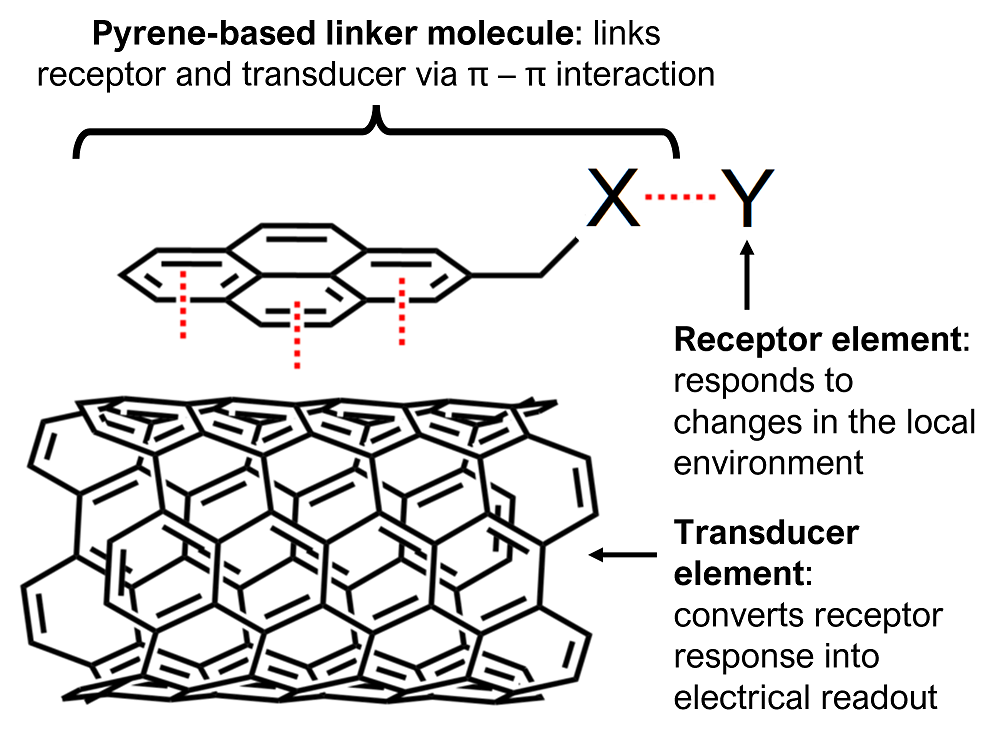
\includegraphics[width=0.8\textwidth,height=\textheight]{figures/ch6/pyrene-cnt.png}

}

\caption{\label{fig-pi-interaction-cnt}Attachment of pyrene-based linker
molecule pyrene-X and receptor Y to a carbon nanotube, representing the
transducer element of a field-effect transistor. Source: Adapted from
\autocite{Carbonnanotube}.}

\end{figure}

\(\pi\)-stacking or \(\pi-\pi\) interaction is often used to describe a
type of non-covalent bonding which occurs due to dispersion forces
between unsaturated polycyclic molecules \autocite{Perez2015}. It has
been argued that this label is unhelpfully specific and a
misrepresentation of what can be simply classed as a type of Van Der
Waals bonding \autocite{Martinez2012,Perez2015}. However, as the use of
the term is widespread in the literature, it is also used here for the
sake of clarity. Carbon nanotubes and graphene consist of a network of
carbon atoms attached to each other by sp\(^{2}\) hybrid orbitals in a
polycyclic structure. They are therefore able to strongly interact with
linker molecules with aromatic moieties, such as pyrene
\autocite{Hermanson2013-16,Perez2015,Mishyn2022}.
Figure~\ref{fig-pi-interaction-cnt} is a visual demonstration of the
relationship between the pyrene-based linker molecule with the
transducer and receptor elements. A wide range of pyrene-based linker
molecules have been used for non-covalent modification of carbon
nanotubes and graphene \autocite{Zhou2019}. \(\pi\)-stacking with pyrene
is the bonding mechanism underlying all the functionalisation processes
in this thesis.

\hypertarget{sec-PBASE}{%
\section{Attachment of 1-Pyrenebutanoic Acid N-Hydroxysuccinimide
Ester}\label{sec-PBASE}}

\hypertarget{comparing-attachment-methods}{%
\subsection{Comparing Attachment
Methods}\label{comparing-attachment-methods}}

\begin{figure}

\begin{minipage}[t]{0.47\linewidth}

{\centering 

\raisebox{-\height}{

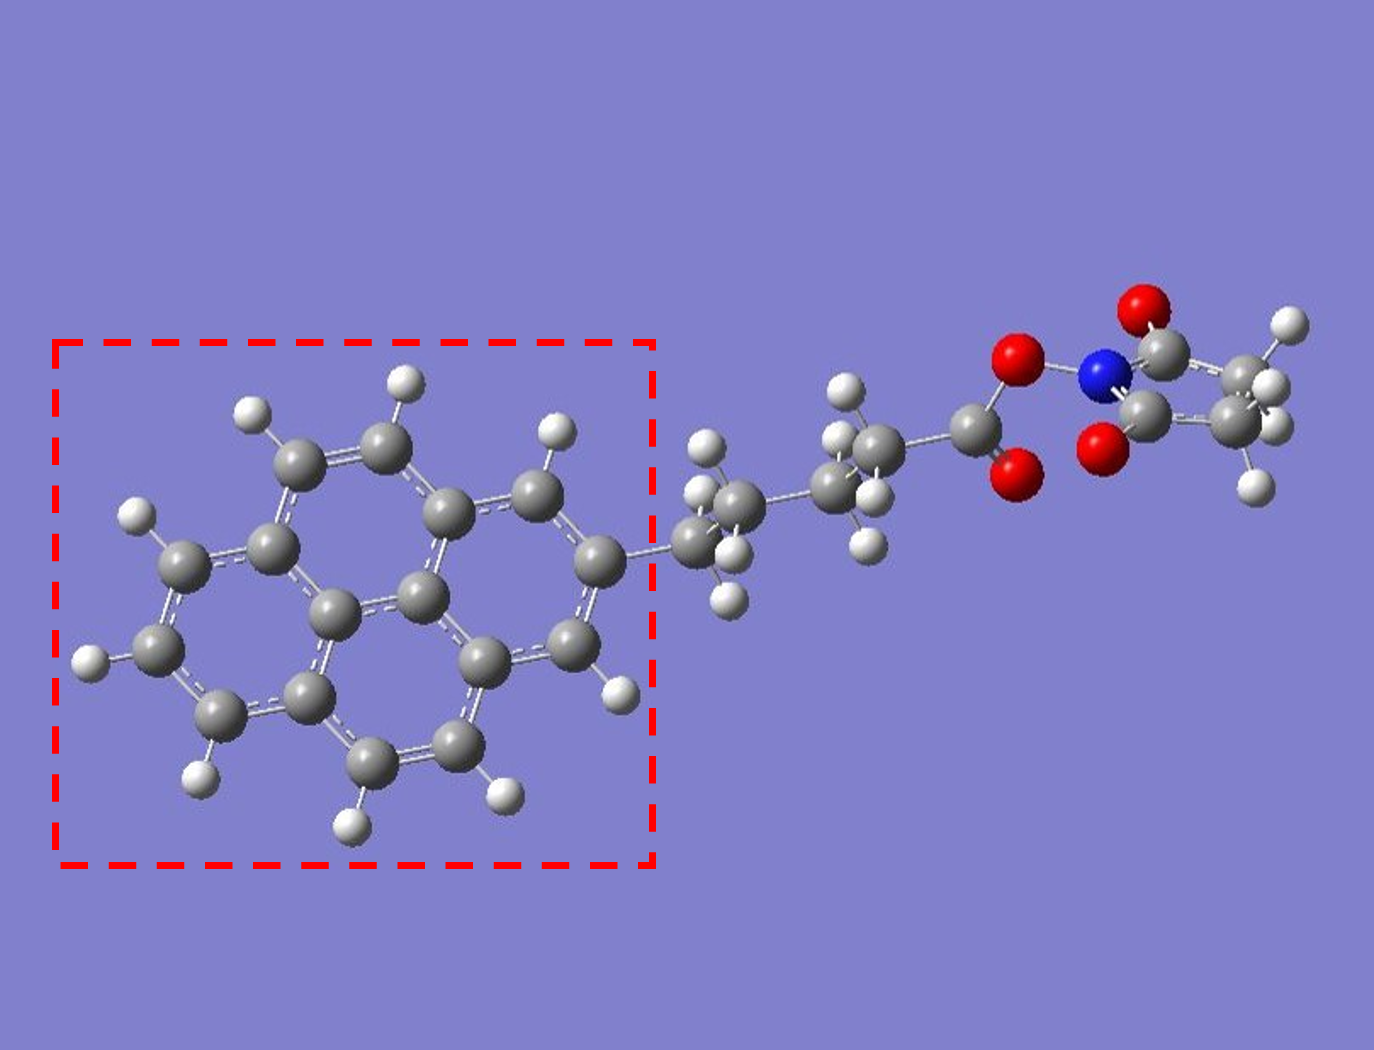
\includegraphics{figures/ch6/pbase_stable_1_pyrene.png}

}

}

\subcaption{\label{fig-pbase-stable-1}}
\end{minipage}%
%
\begin{minipage}[t]{0.05\linewidth}

{\centering 

~

}

\end{minipage}%
%
\begin{minipage}[t]{0.47\linewidth}

{\centering 

\raisebox{-\height}{

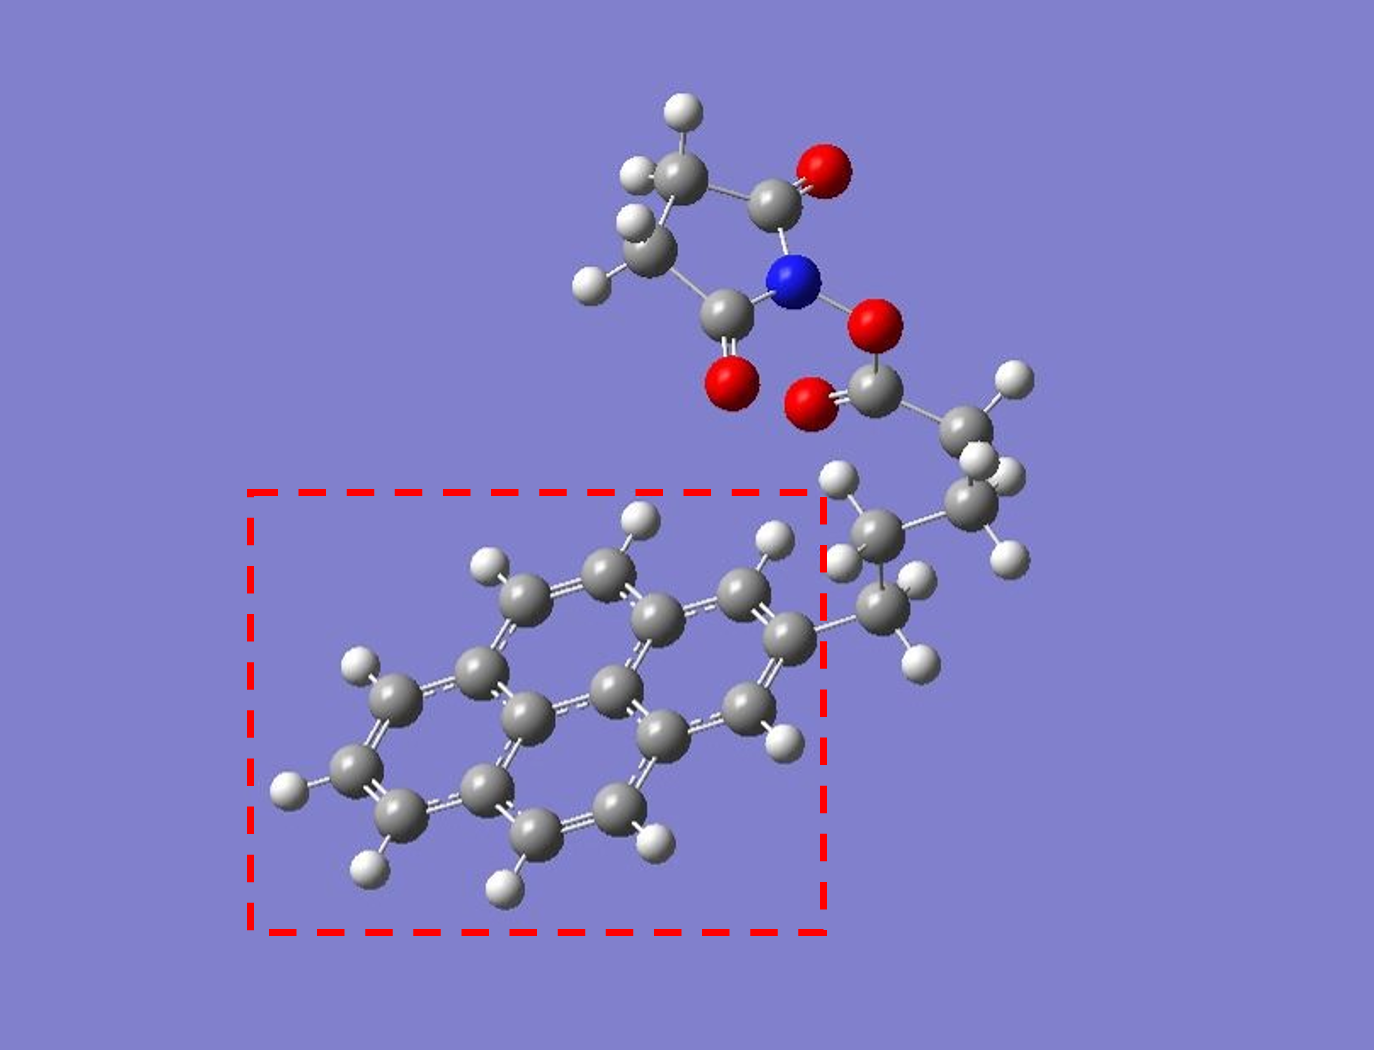
\includegraphics{figures/ch6/pbase_stable_2_pyrene.png}

}

}

\subcaption{\label{fig-pbase-stable-2}}
\end{minipage}%

\caption{\label{fig-pbase-structure}Two conformations of PBASE molecule
with geometry optimised via \emph{ab initio} calculations performed with
Gaussian 16 software \autocite{g16}. White balls correspond to hydrogen,
grey to carbon, red to oxygen and blue to nitrogen. The pyrene moiety is
highlighted in the image with a red dashed outline.}

\end{figure}

1-pyrenebutanoic acid N-hydroxysuccinimide ester (also known
commercially and in the literature both as 1-pyrenebutyric acid
N-hydroxysuccinimide ester and 1-pyrenebutanoic acid succinimidyl ester;
acronyms include PBASE, PBSE, PyBASE, PASE, PYSE, PSE, Pyr-NHS and
PANHS) is a aromatic molecule commonly used for tethering biomolecules
to the carbon rings of graphene and carbon nanotubes. Using
computational modelling, two locally stable molecular conformations were
found to exist, a straight (Figure~\ref{fig-pbase-stable-1}) and bent
(Figure~\ref{fig-pbase-stable-2}) structure. The conformation in
Figure~\ref{fig-pbase-stable-1} has a Hartree-Fock energy of -3427728.67
kJ/mol, while the conformation in Figure~\ref{fig-pbase-stable-2} has a
Hartree-Fock energy of -3427729.66 kJ/mol. The difference between
computed Hartree-Fock energies is 1.0 kJ/mol, small enough that the
existence of both molecular conformations is physically feasible.
Similar straight and bent structures have previously been modelled for
PBASE attached to graphene \autocite{Oishi2022}.

\newpage
\KOMAoptions{paper=landscape,pagesize}

\hypertarget{tbl-pbase-functionalisation}{}
\begin{longtable}[]{@{}lllllll@{}}
\caption{\label{tbl-pbase-functionalisation}Comparison of PBASE
functionalisation processes used for immobilisation of proteins and
aptamers onto carbon nanotubes and graphene. Experimentally optimised
variables are marked with a star (*). Blank entries indicate there was
no mention of the parameter in a particular paper.}\tabularnewline
\toprule\noalign{}
Solvent & Channel & Conc. (mM) & Incubation type & Time (hr) & Rinse
steps & References \\
\midrule\noalign{}
\endfirsthead
\toprule\noalign{}
Solvent & Channel & Conc. (mM) & Incubation type & Time (hr) & Rinse
steps & References \\
\midrule\noalign{}
\endhead
\bottomrule\noalign{}
\endlastfoot
DMF & CNT & 5 & Immersed & 1 & PBS & Maehashi, 2007.
\cite{Maehashi2007} \\
& & 6 & Immersed & 1 & DMF, PBS & García-Aljaro, 2010.
\cite{Garcia-Aljaro2010} \\
& & 6 & Immersed & 1 & DMF & Chen, 2001. \cite{Chen2001} \\
& & 6 & Immersed & 1 & DMF & Cella, 2010. \cite{Cella2010} \\
& & 6 & Immersed & 1 & DMF & Das, 2011. \cite{Das2011} \\
& & 6 & - & 2 & DMF & Besteman, 2003. \cite{Besteman2003} \\
& Graphene & - & - & 2 & DMF & Tsang, 2019. \cite{Tsang2019} \\
& & - & - & 20 & - & Wiedman, 2017. \cite{Wiedman2017} \\
& & 0.2 & Immersed & 20 & DMF, IPA, DI water & Gao, 2018.
\cite{Gao2018} \\
& & 1 & Dropcast & 6 & DMF, IPA, DI water & Nekrasov, 2021.
\cite{Nekrasov2021} \\
& & 5 & Immersed & 1 & DMF, DI water & Hwang, 2016. \cite{Hwang2016} \\
& & 5* & Immersed & 3* & DMF & Hao, 2020. \cite{Hao2020} \\
& & 5 & Immersed & 4* & DMF, DI water & Mishyn, 2022.
\cite{Mishyn2022} \\
& & 6 & Dropcast & 2 & DMF, DI water & Nur Nasufiya, 2020.
\cite{NurNasyifa2020} \\
& & 10 & Dropcast & 2 & DMF, DI water & Campos, 2019.
\cite{Campos2019} \\
& & 10 & Immersed & 2 & DMF, PBS & Kuscu, 2020. \cite{Kuscu2020} \\
& & 10 & Immersed & 1 & DMF & Xu, 2017. \cite{Xu2017} \\
& & 10 & Immersed & 12 & DMF, EtOH, DI water & Khan, 2020.
\cite{Khan2020} \\
& & 50 & Immersed & 4* & MeOH & Wang, 2020. \cite{Wang2020} \\
2-Methoxyethanol & Graphene & 1 & Immersed & 1 & DI water & Ono, 2020.
\cite{Ono2020} \\
Methanol & CNT & 1 & Immersed & 1 & MeOH, DI water & Zheng, 2016.
\cite{Zheng2016} \\
& & 1 & Immersed & 2 & MeOH & Kim, 2009. \cite{Kim2009} \\
& & 100 & Dropcast & 1 & DI water & Yoo, 2022. \cite{Yoo2022} \\
& Graphene & 5 & Immersed & 2 & - & Sethi, 2020. \cite{Sethi2020} \\
& & 5 & Immersed & 1 & MeOH, PBS & Ohno, 2010. \cite{Ohno2010} \\
DMSO & CNT & 10 & - & 1 & DI water & Lopez, 2015. \cite{Lopez2015} \\
& & 10 & Immersed & 1 & PBS & Strack, 2013. \cite{Strack2013} \\
\end{longtable}

\newpage
\KOMAoptions{paper=portrait,pagesize}

The pyrene moiety, highlighted with a red dashed outline in
Figure~\ref{fig-pbase-stable-1}-b, non-covalently bonds to the carbon
rings of the carbon nanotube and graphene surface. The
N-hydroxysuccinimide (NHS) ester group, seen on the right-hand side of
Figure~\ref{fig-pbase-structure}, is highly reactive with amine groups.
It can undergo a nucleophilic substitution reaction with amines attached
to proteins or aptamers, tethering these biomolecules via an amide or
imide bond
\autocite{Chen2001,Hermanson2013-16,Hermanson2013-3,Mishyn2022}.

The non-covalent functionalisation of proteins onto a single-walled
carbon nanotube using PBASE was first reported by Chen \emph{et al.} in
2001 \autocite{Chen2001}. Two successful methods for protein
functionalisation and immobilisation were reported, with the only
differences being the solvent used to dissolve the PBASE powder (DMF,
methanol) and the final concentration of the resulting solutions (6 mM,
1 mM respectively). PBASE powder appears to dissolve poorly in methanol
at higher concentrations, which might explain the use of different
concentrations of PBASE in each solvent. An extensive comparison of
methods used in the literature for PBASE functionalisation of carbon
nanotube and graphene devices with aptamers and proteins is given in
Table~\ref{tbl-pbase-functionalisation}. Several listed works directly
cite Chen \emph{et al.} when discussing functionalisation with PBASE
\autocite{Besteman2003,Cella2010,Campos2019,Zheng2016,Ohno2010}. The
other works listed do not explicitly reference Chen \emph{et al.} in
their methodology; however, the frequency of methods detailing the use
of 6 mM PBASE in dimethylformamide (DMF) and 1 mM PBASE in methanol
indicate that these processes are largely copying the process used by
Chen \emph{et al.}.

However, it is also apparent from
Table~\ref{tbl-pbase-functionalisation} that there is a large degree of
variation in the methods used for PBASE functionalisation. Various
electrical characterisation, microscopy and spectroscopy techniques have
been used to demonstrate successful functionalisation. Until recently,
there has been little justification provided for the selection of
variables used in the functionalisation procedure (e.g.~length of time
submerged in solvent containing PBASE), despite the wide-ranging use of
this process in the literature \autocite{Hinnemo2017,Zhen2018,Wang2020}.
This is surprising, given that the sensitivity of functionalised devices
is considered to be closely related to the density of surface
functionalisation \autocite{White2008,Hermanson2013-3,Chen2014}.
Furthermore, a detailed investigation of PBASE functionalisation process
variables has only been undertaken for graphene-based devices
\autocite{Zhen2018,Hao2020,Wang2020,Mishyn2022}.

Zhen \emph{et al.} \autocite{Zhen2018}, Wang \emph{et al.}
\autocite{Wang2020} and Mishyn \emph{et al.} \autocite{Mishyn2022} have
all claimed that carefully tuning the surface concentration of PBASE is
required to avoid multilayer coverage of the graphene surface, as this
negatively impacts sensing. Mishyn \emph{et al.} \autocite{Mishyn2022}
used cyclic voltammetry to demonstrate that less receptor attachment to
the graphene surface occurs when multiple layers of PBASE are present.
However, none of these groups have presented analyte sensing results
from their functionalised graphene devices. In contrast, Hao \emph{et
al.} \autocite{Hao2020} found that maximising the PBASE surface coverage
of a channel resulted in more sensitive aptameric sensing, thereby
reaching the opposite conclusion. The inconsistency in these recent
findings mean more work is needed to understand the PBASE
functionalisation process to achieve optimal biosensor sensitivity. It
may also be the case that a specific functionalisation process is
required for optimal sensitivity with the use of a specific type of
receptor.

\begin{figure}

\begin{minipage}[t]{\linewidth}

{\centering 

\raisebox{-\height}{

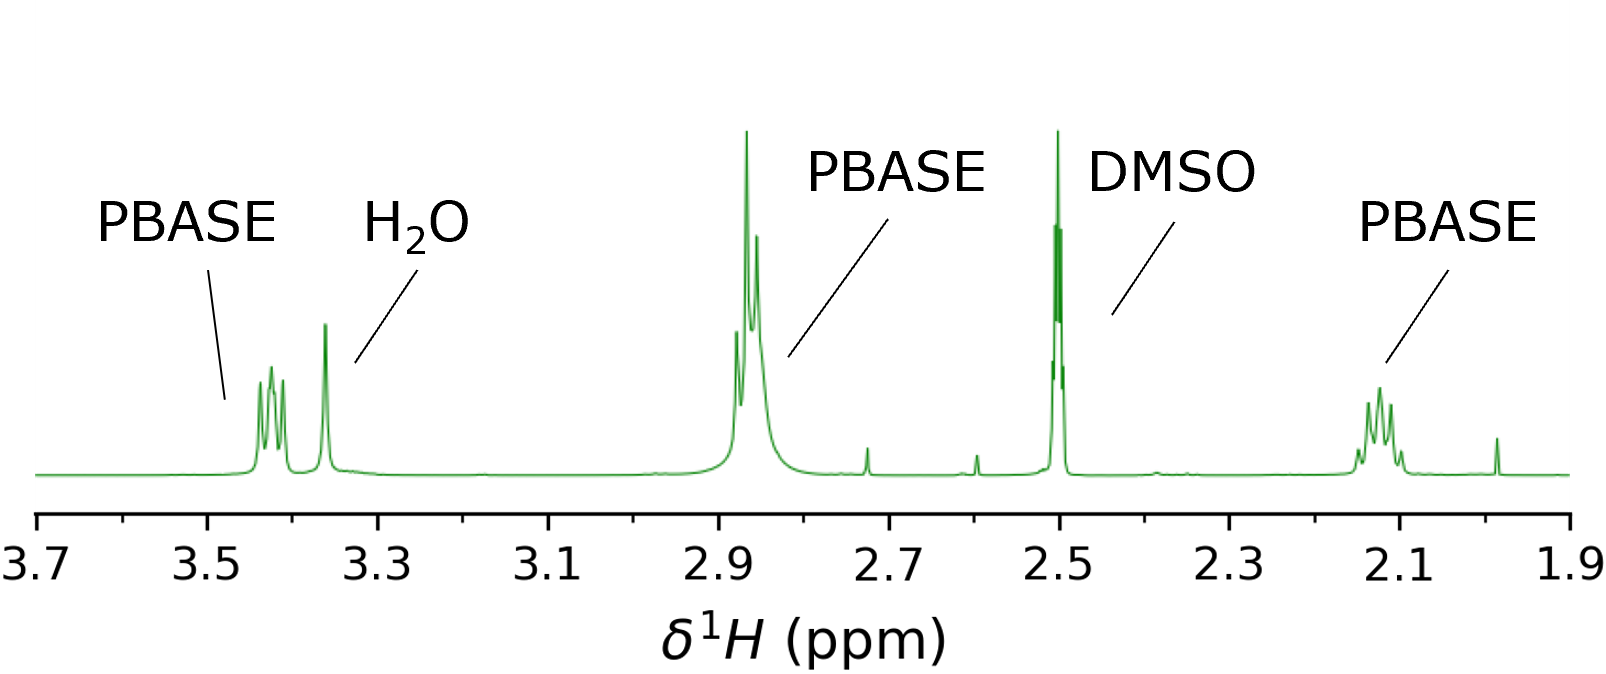
\includegraphics{figures/ch6/labelled_modified_sigma_pbase_nmr.png}

}

}

\subcaption{\label{fig-sigma-nmr}}
\end{minipage}%
\newline
\begin{minipage}[t]{\linewidth}

{\centering 

\raisebox{-\height}{

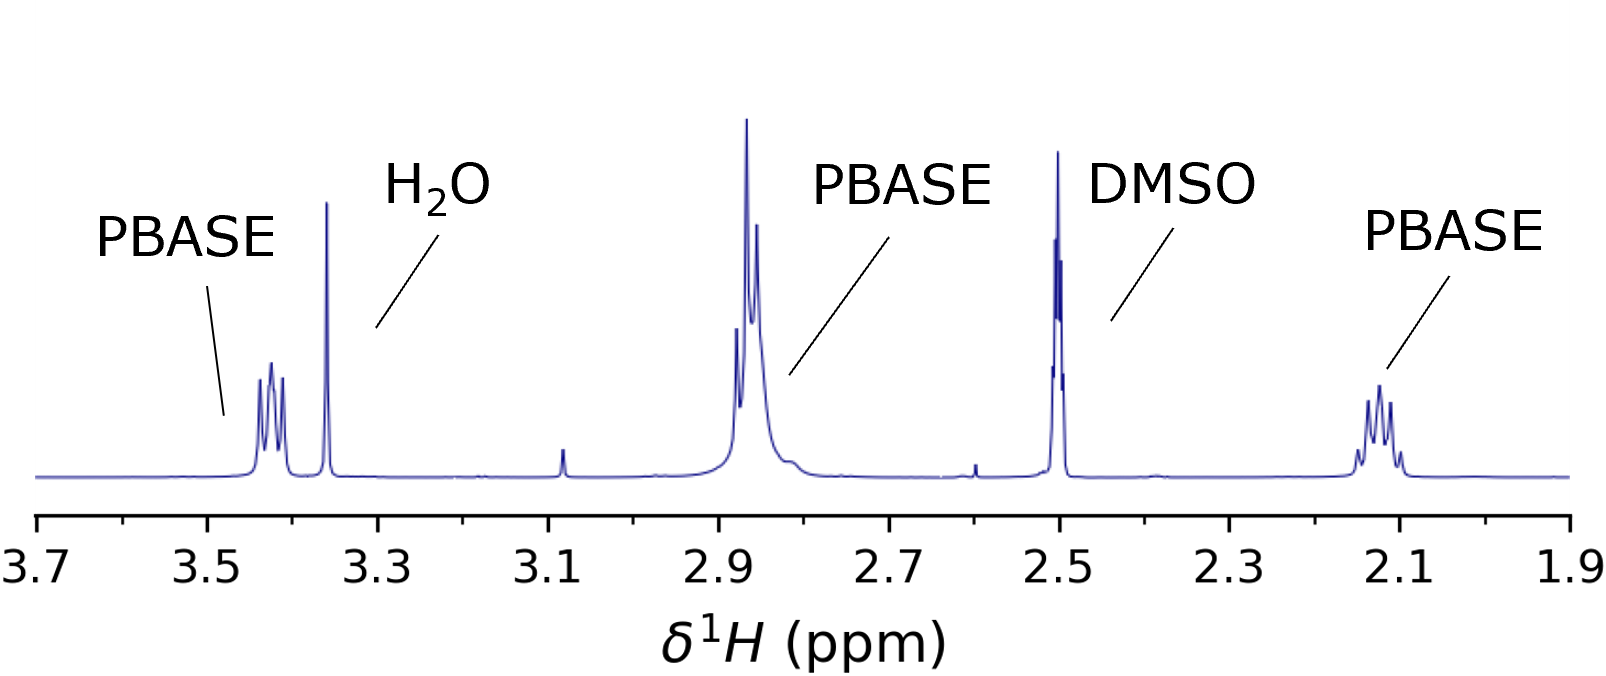
\includegraphics{figures/ch6/labelled_modified_setareh_pbase_nmr.png}

}

}

\subcaption{\label{fig-setareh-nmr}}
\end{minipage}%
\newline
\begin{minipage}[t]{\linewidth}

{\centering 

\raisebox{-\height}{

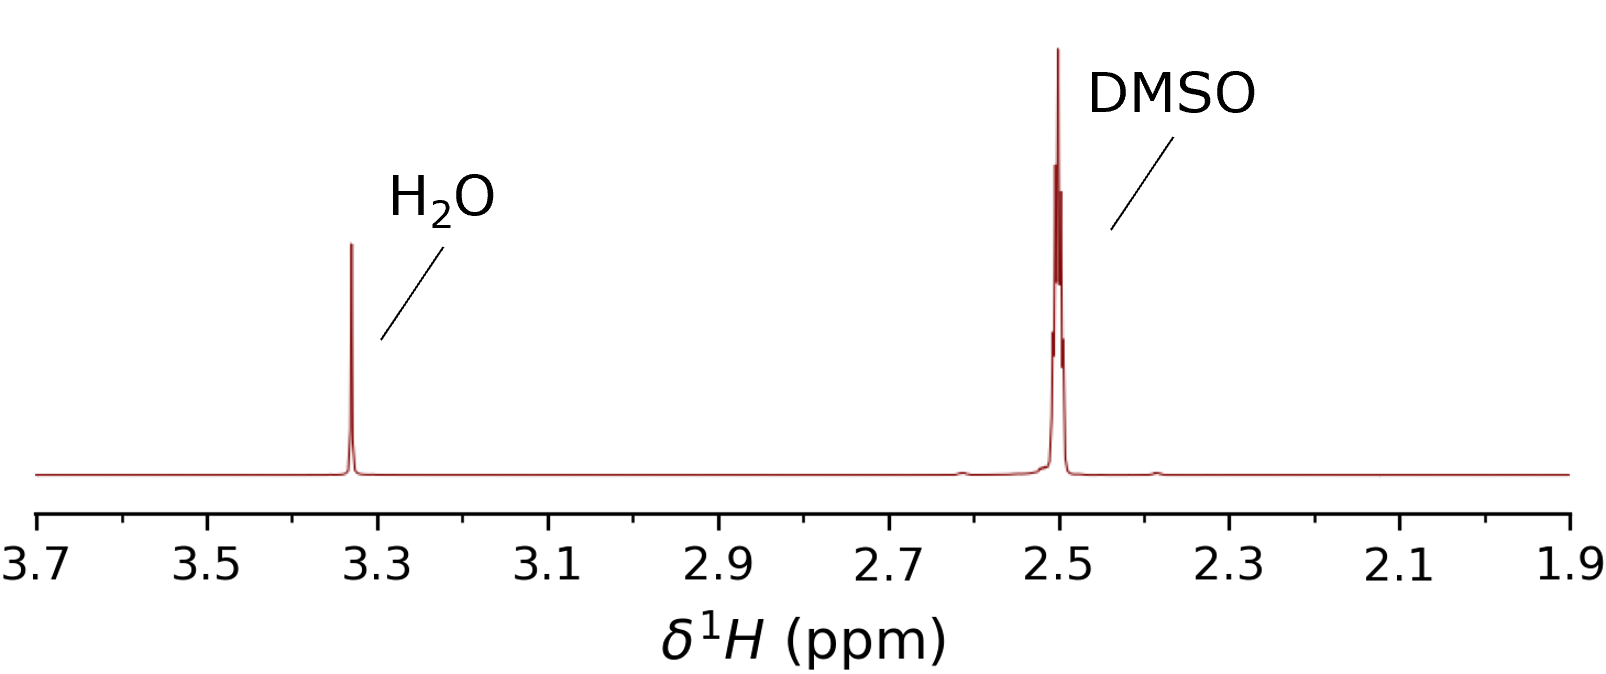
\includegraphics{figures/ch6/labelled_modified_dmso_nmr.png}

}

}

\subcaption{\label{fig-dmso-nmr}}
\end{minipage}%

\caption{\label{fig-pbase-nmr}\(^{1}\)H Nuclear Magnetic Resonance (NMR)
spectra, performed with DMSO-d\(_6\) used as the NMR solvent. (a) and
(b) show NMR spectrum for commercially purchased PBASE, from
Sigma-Aldrich and Setareh Biotech respectively, while (c) shows the
blank spectrum taken with only DMSO-d\(_6\) present (spectra taken by
Jennie Ramirez-Garcia, School of Chemical and Physical Sciences, Te
Herenga Waka - Victoria University of Wellington). Unlabelled peaks
correspond to sample impurities.}

\end{figure}

Once fastened to a bioreceptor via an amide or imide bond, the
attachment to the linker molecule is not easily broken. However, prior
to use in functionalisation processes, the NHS ester may react with any
water present (hydrolysis). This reaction converts PBASE to
1-pyrenebutyric acid (PBA), leaving it unavailable to react further with
amine groups \autocite{Hermanson2013-3,Hermanson2013-5,Mishyn2022}. If
the amine group functionalisation is performed within a \(\sim1\) hour
period, with a high concentration of bioreceptor used at close to
neutral pH, competing hydrolysis should not have a significantly adverse
impact on the functionalisation process \autocite{Hermanson2013-3}.
However, if PBASE is exposed to water during storage over a significant
length of time, the presence of
1-Ethyl-3-(3-dimethylaminopropyl)carbodiimide (EDC) can be used to
restore the NHS ester and enable the substitution reaction to take place
(see discussion of PBA/EDC in Section~\ref{sec-PBA}).

\hypertarget{examining-1-pyrenebutanoic-acid-n-hydroxysuccinimide-ester-purity}{%
\subsection{Examining 1-Pyrenebutanoic Acid N-Hydroxysuccinimide Ester
Purity}\label{examining-1-pyrenebutanoic-acid-n-hydroxysuccinimide-ester-purity}}

I purchased PBASE from two suppliers, Sigma-Aldrich and Setareh Biotech.
Sigma recommended DMF and methanol as suitable solvents for dissolving
PBASE, alongside chloroform and dimethyl sulfoxide (DMSO). Setareh
Biotech indicated methanol can be used for dissolving PBASE. The two
suppliers had conflicting information for suitable storage of PBASE,
with Sigma recommending room temperature storage while Setareh Biotech
recommends storage of \(-5\) to \(-30 ^\circ \text{C}\) and protection
from light and moisture. I used nuclear magnetic resonance (NMR)
spectroscopy to verify the purity of PBASE from various suppliers. As
water can react with PBASE to form unwanted byproducts, it appears that
protection from moisture is particularly important. A particular
emphasis was placed on detecting water presence in the received samples,
considering the long travel time of the PBASE with uncertain storage
conditions.

Figure~\ref{fig-pbase-nmr} compares the shapes of hydrogen NMR spectra
of PBASE from each supplier when dissolved in deuterated DMSO, alongside
a blank deuterated DMSO spectrum. Both PBASE samples possessed
characteristic chemical shift features between \(2.1-2.2\) ppm,
\(2.8-2.9\) ppm, and \(3.4-3.5\) ppm. These chemical shifts roughly
correspond to those seen in previous NMR spectra for PBASE
\autocite{NMR2}. The feature at 2.50 ppm represents the deuterated DMSO
solvent, while the single peak between \(3.3-3.4\) ppm represents the
water present in the sample. By comparing the area of these peaks, a
rough estimate of the amount of water originally present in the PBASE
sample can be obtained. The H\(_{2}\)O:DMSO ratio is 1:7 in the blank
spectrum, but \(\sim\) 1:3 in the provided samples, possibly indicating
the introduction of water to the PBASE during production or storage.
However, DMSO is strongly hygroscopic and slight differences in DMSO
storage time, as well as differences in humidity during sample
preparation, may have had a significant impact on this result
\autocite{Lebel1962}. Other impurities are also seen on both PBASE
spectra, though their small size indicates they make up only a small
percentage of each sample. Strack \emph{et al.} \autocite{Strack2013}
recommend leaving frozen PBASE at room temperature for 15 minutes before
exposing it to air to prevent condensation near the PBASE, as this can
cause unnecessary \(H_2O\) contamination.

\hypertarget{electrical-characterisation}{%
\subsection{Electrical
Characterisation}\label{electrical-characterisation}}

\begin{figure}

\begin{minipage}[t]{0.50\linewidth}

{\centering 

\raisebox{-\height}{

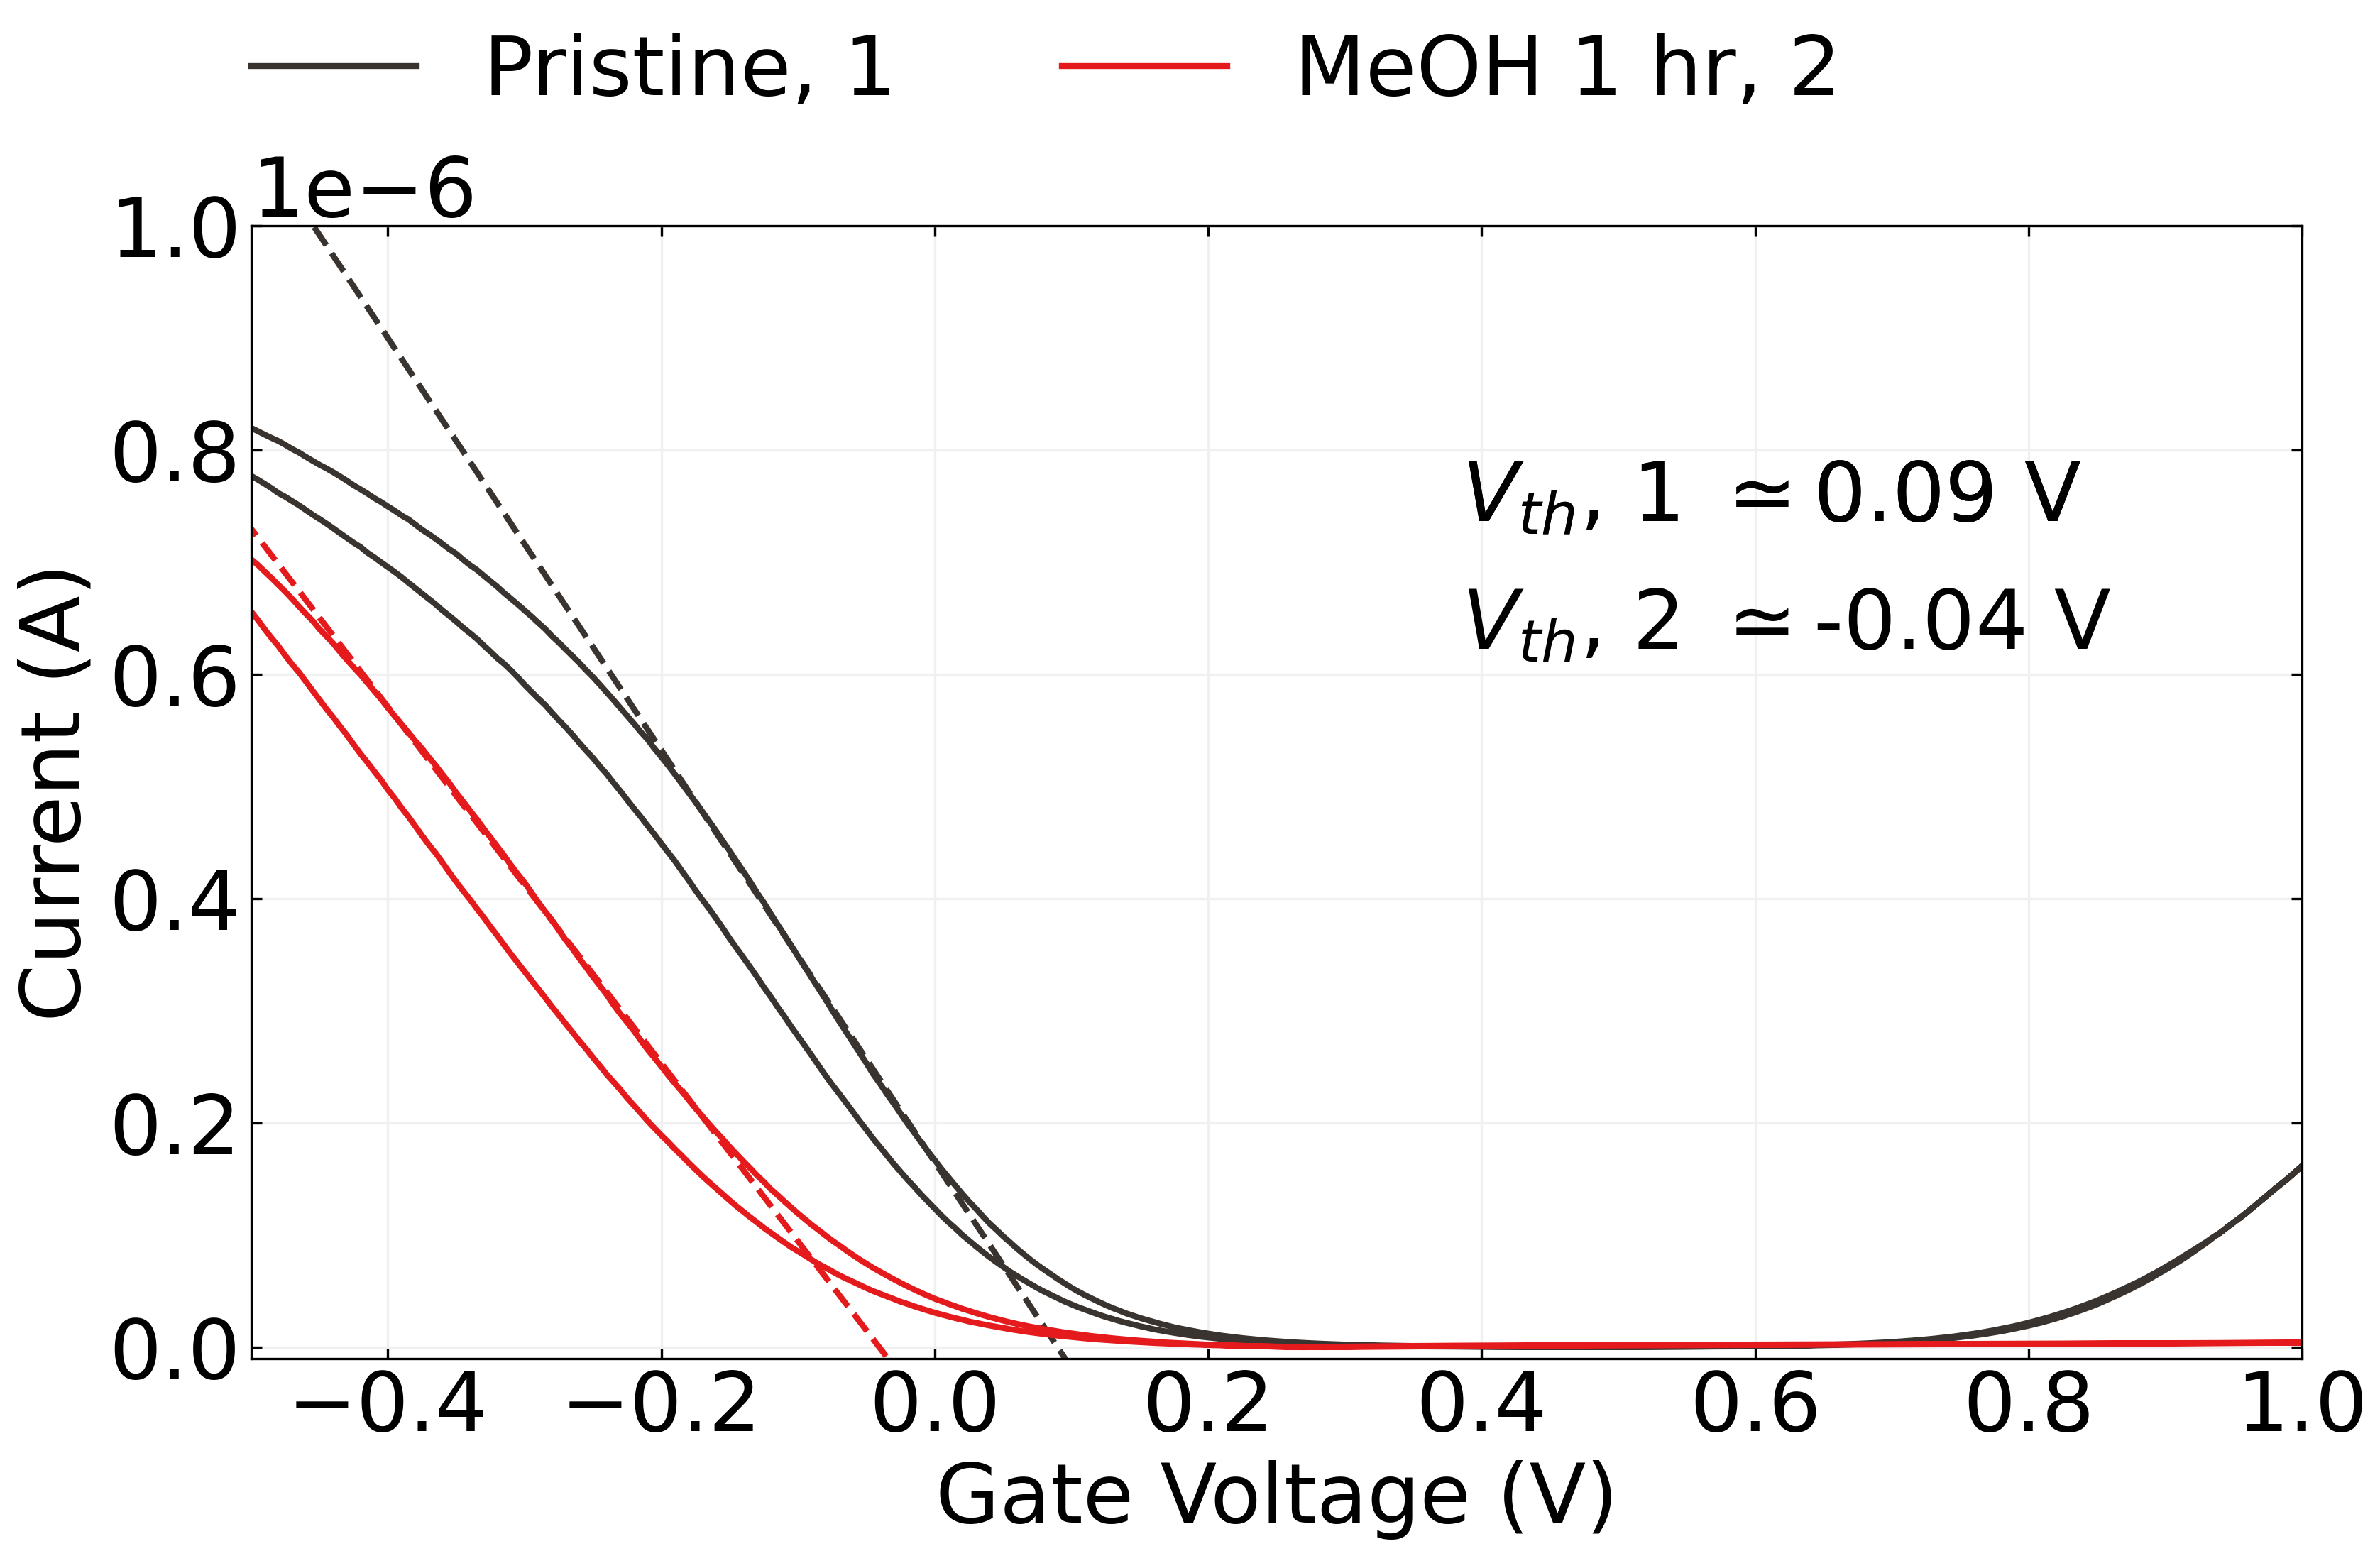
\includegraphics{figures/ch6/Q23D5_ch1_MeOHonly.png}

}

}

\subcaption{\label{fig-meoh-only-tx}}
\end{minipage}%
%
\begin{minipage}[t]{0.50\linewidth}

{\centering 

\raisebox{-\height}{

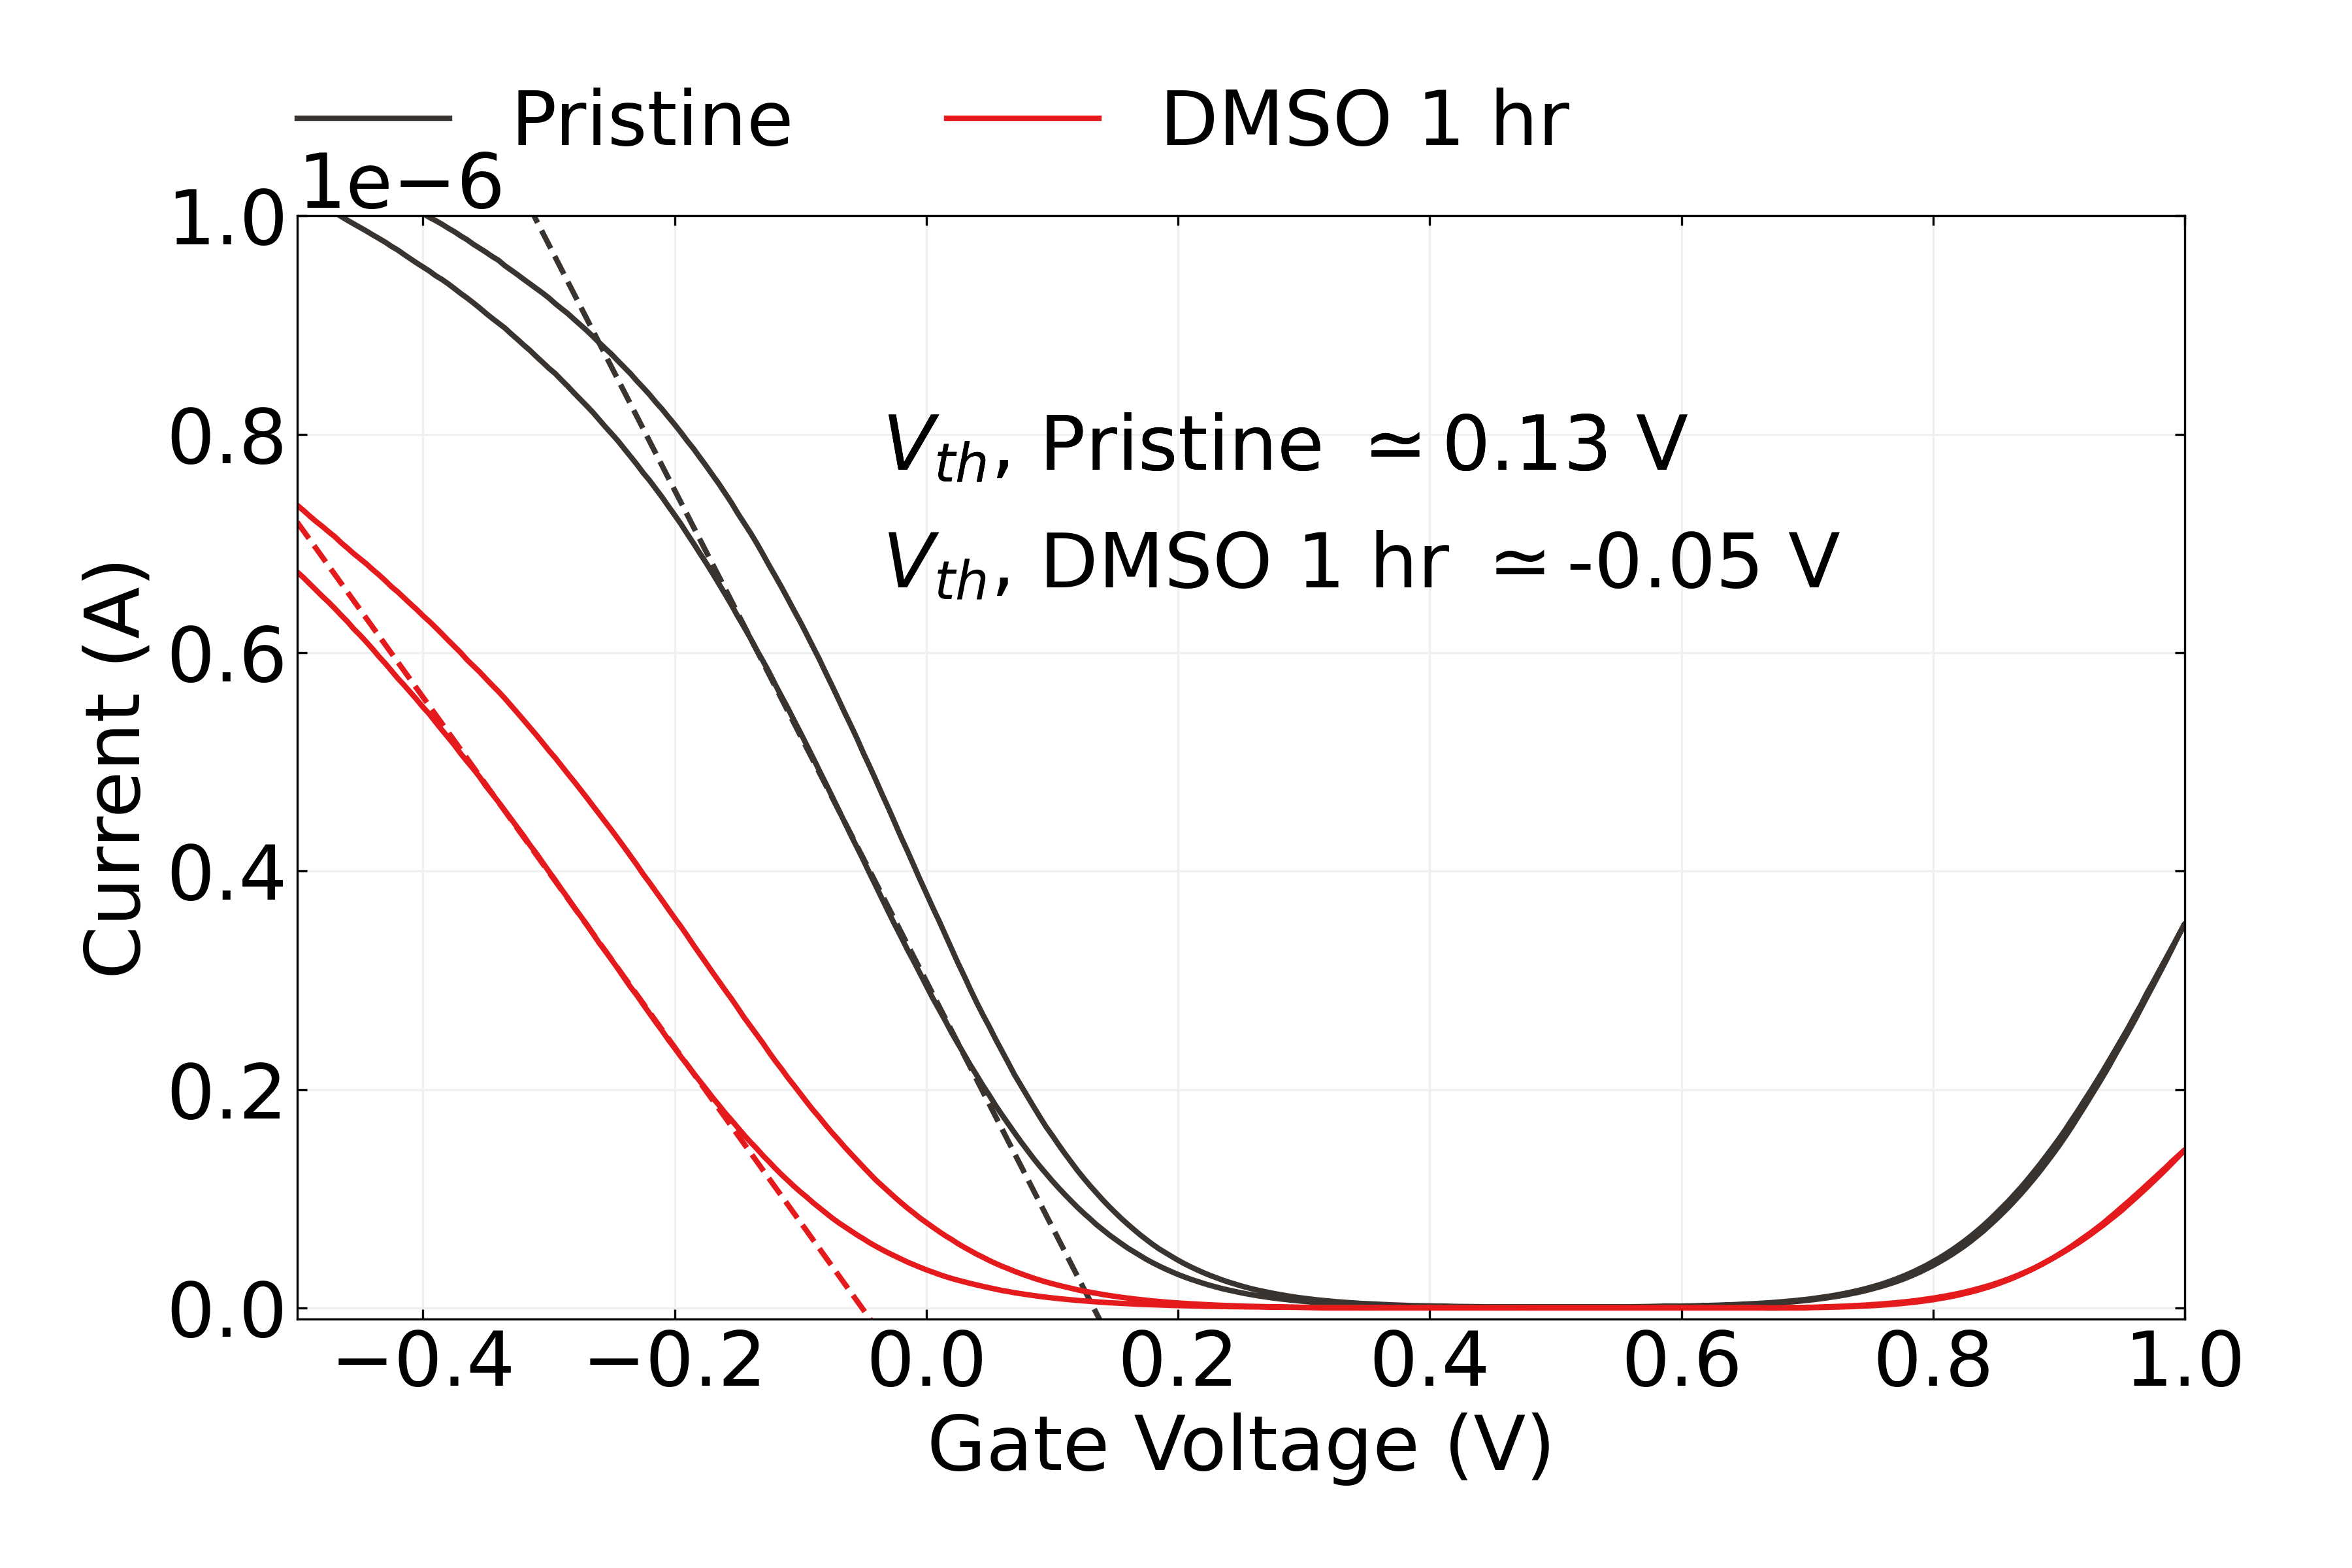
\includegraphics{figures/ch6/Q23D12_ch1_DMSOonly.png}

}

}

\subcaption{\label{fig-dmso-only-tx}}
\end{minipage}%
\newline
\begin{minipage}[t]{0.50\linewidth}

{\centering 

\raisebox{-\height}{

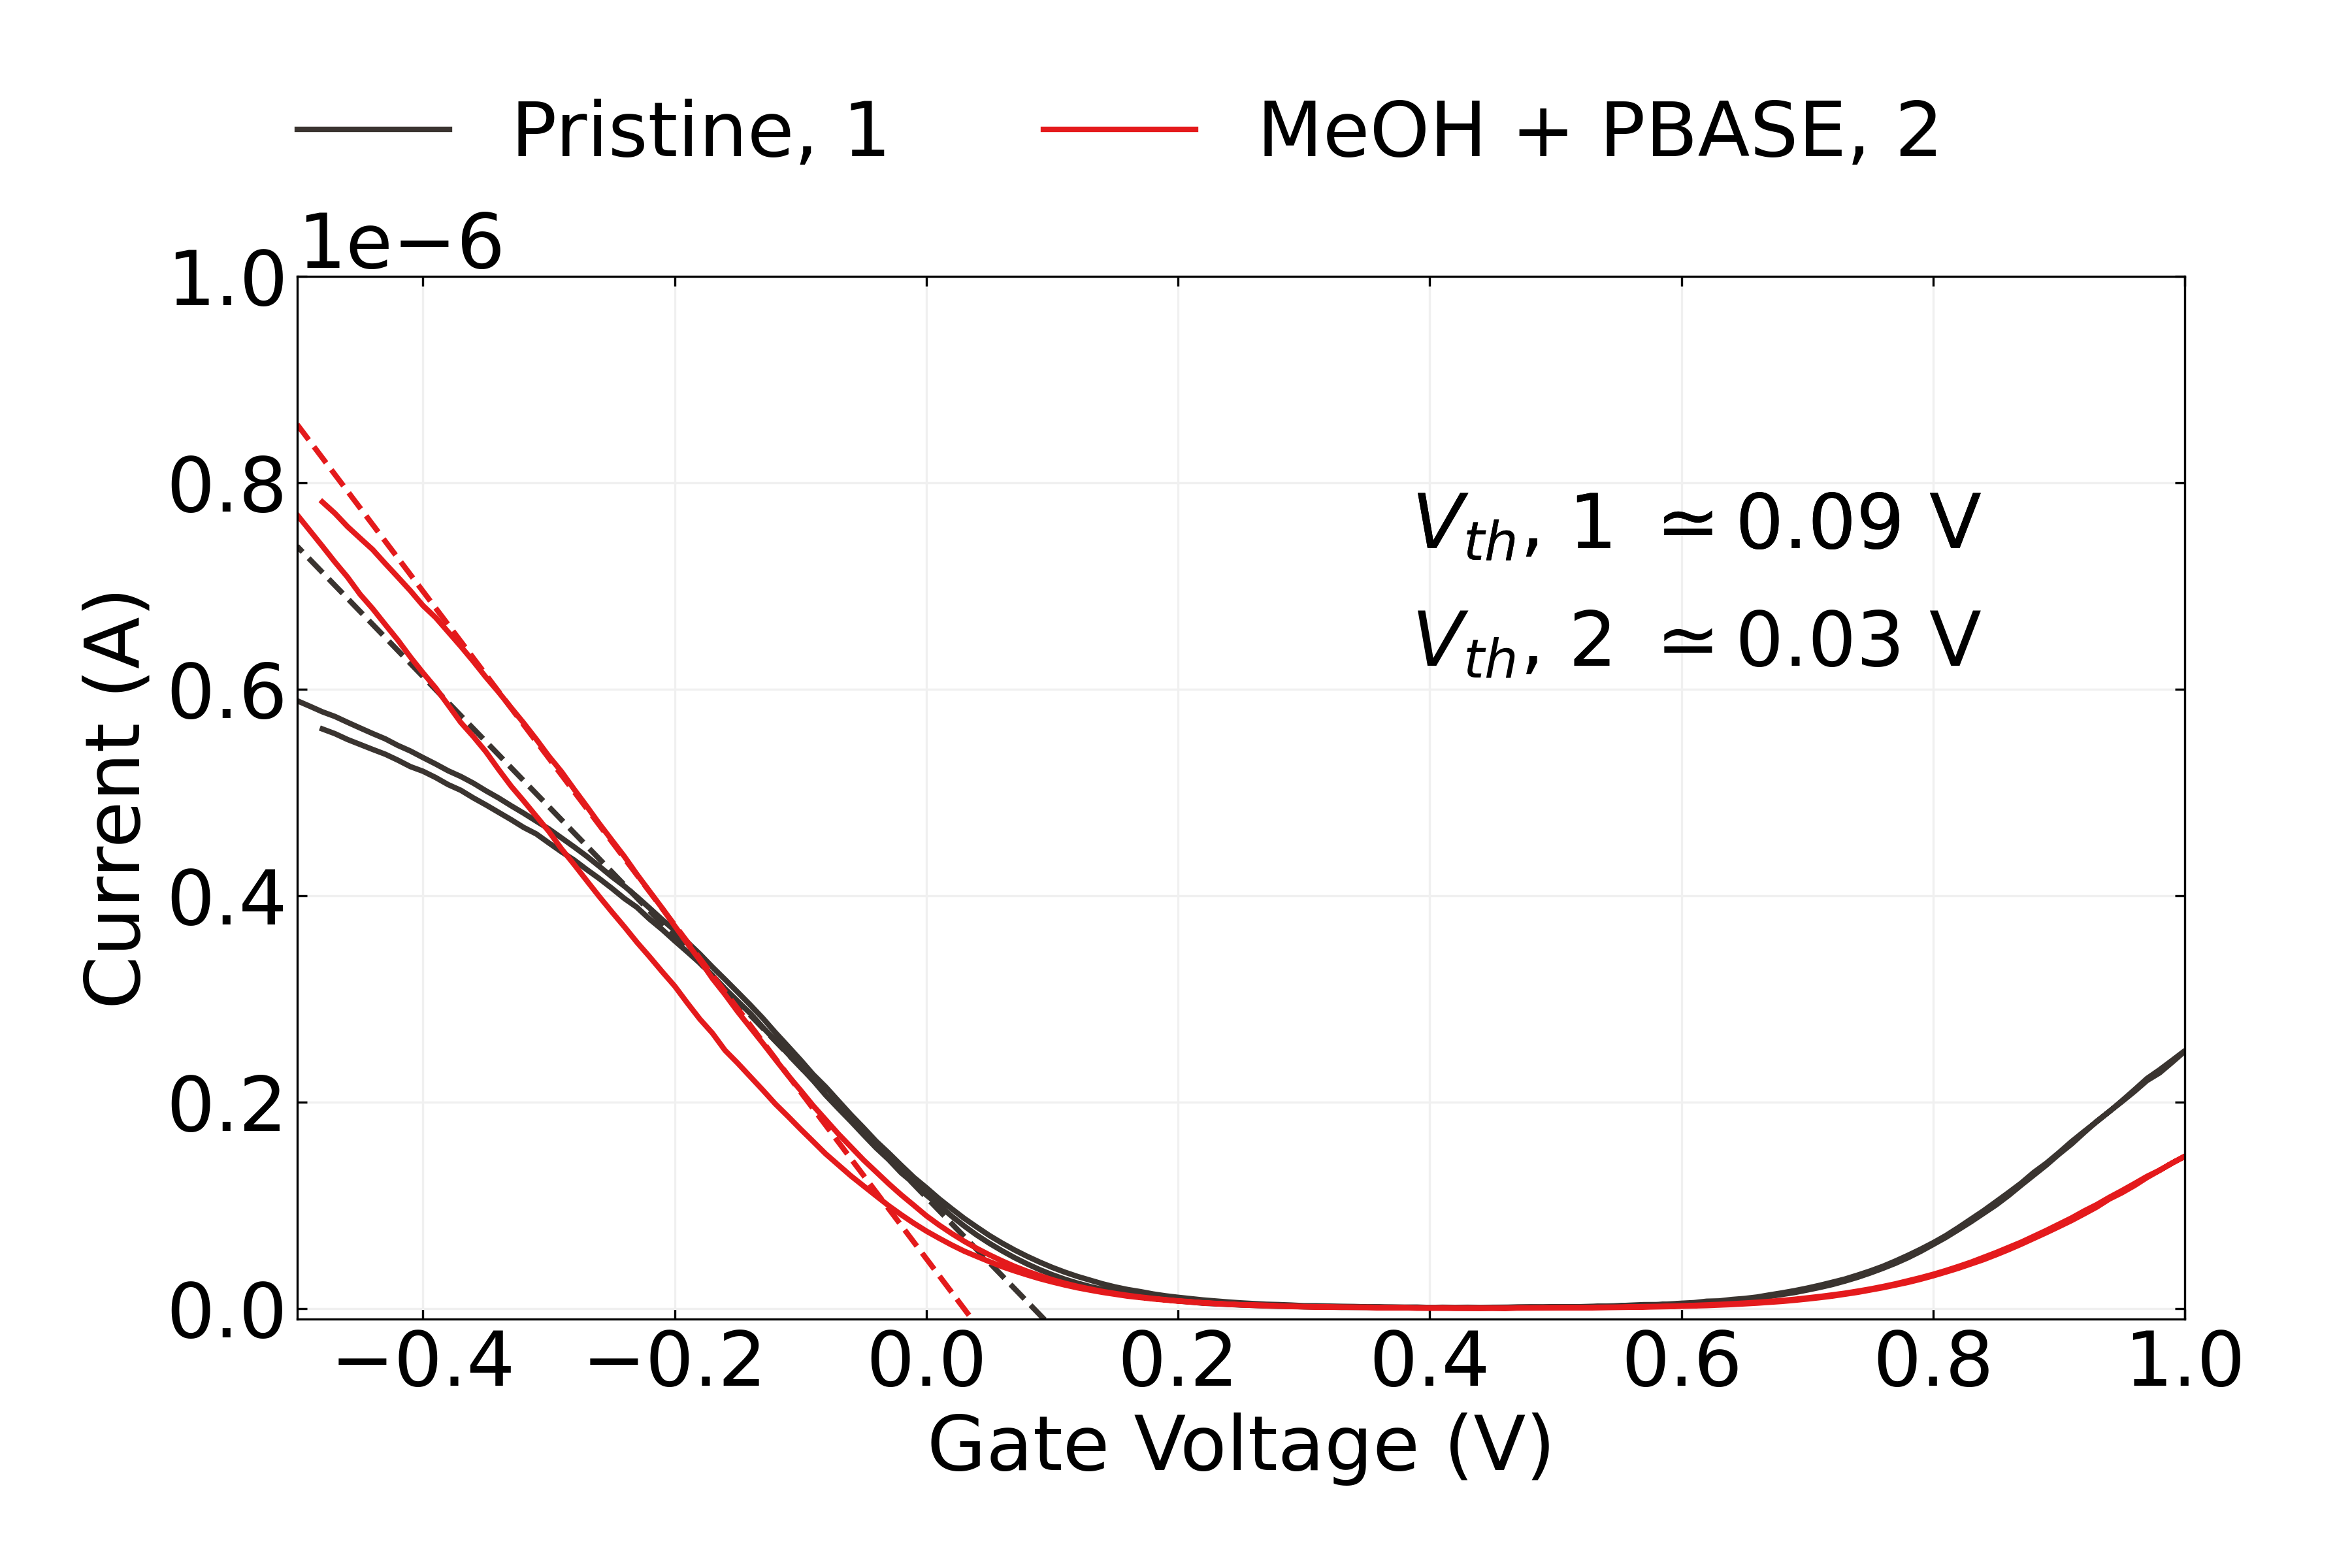
\includegraphics{figures/ch6/Q2C6_ch2_MeOHPBASE.png}

}

}

\subcaption{\label{fig-meoh-pbase-tx}}
\end{minipage}%
%
\begin{minipage}[t]{0.50\linewidth}

{\centering 

\raisebox{-\height}{

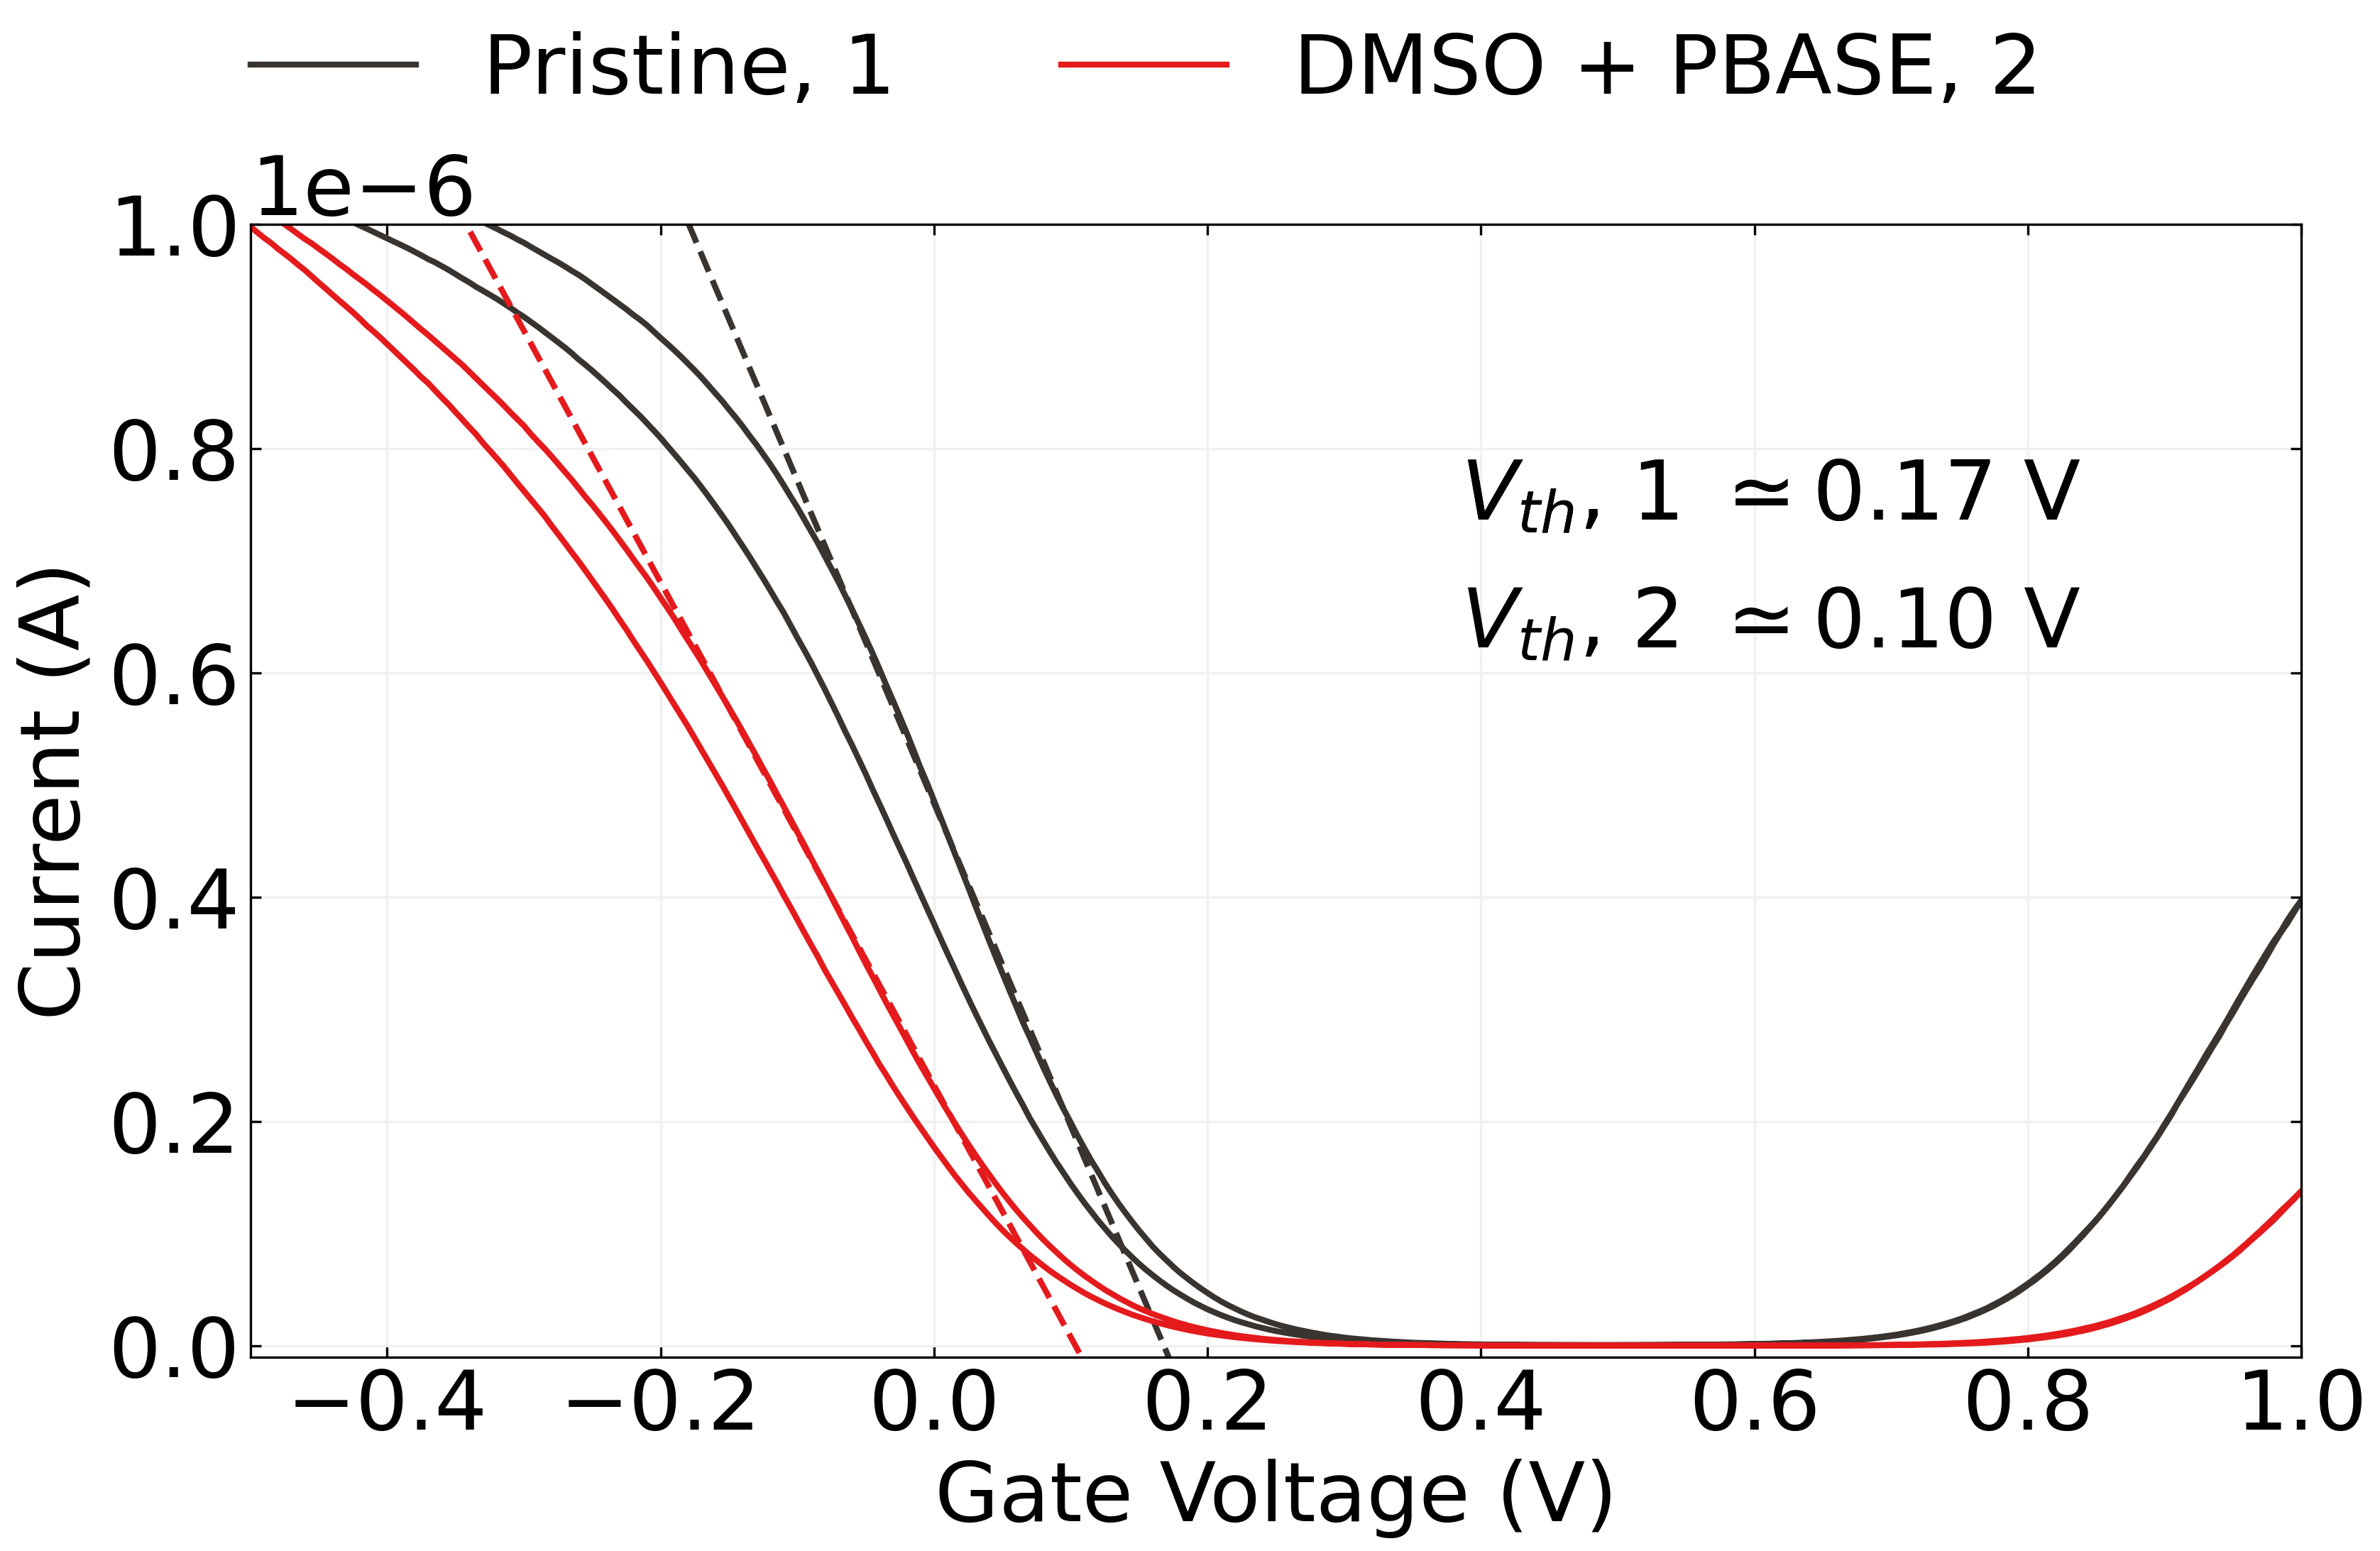
\includegraphics{figures/ch6/Q23D7_ch3_DMSOPBASE.png}

}

}

\subcaption{\label{fig-dmso-pbase-tx}}
\end{minipage}%

\caption{\label{fig-PBASE-vs-solvent-only}The electrical transfer
characteristics of carbon nanotube transistors (V\_\{ds\} = 100 mV)
before and after being submerged in methanol (a) or dimethyl sulfoxide
(b) for one hour and subsequently rinsed with deionised water. The
change in characteristics of similar transistor channels after being
submerged in these same solvents containing 1 mM PBASE for one hour and
then rinsed are shown in (c) and (d) respectively. Average threshold
voltages for each transfer characteristic curve are also shown (taking
the average of forward and reverse sweep values).}

\end{figure}

The electrical characteristics of the carbon nanotube or graphene
transistor are often used to verify successful functionalisation and
make a statement about the effect of chemical modification on the
channel. However, this verification usually does not account for the
effect of the solvent on the transistor channel.
Figure~\ref{fig-meoh-only-tx} and Figure~\ref{fig-dmso-only-tx} show
that by exposing a steam-deposited carbon nanotube network channel to
solvents commonly used in PBASE functionalisation processes
(Table~\ref{tbl-pbase-functionalisation}), such as methanol (MeOH) or
dimethyl sulfoxide (DMSO), a significant negative shift in channel
threshold voltage occurs even after thorough rinsing with deionised
water. Besteman \emph{et al.} reported observing a similar effect from
prolonged exposure of a single carbon nanotube to dimethylformamide
(DMF) \autocite{Besteman2003}. It appears that the carbon nanotubes have
adsorped solvent which persists even after device cleaning. From the
shape of the change in the transfer curve, it seems the residual polar
solvent molecules capacitively gate the channel
\autocite{Artyukhin2006,Heller2008}.

Furthermore, using the same characterisation process as in this work,
Murugathas \emph{et al.} \autocite{Murugathas2019b} showed that
\(\pi\)-stacking of PBASE onto a solvent-deposited carbon nanotube
network had little effect on channel threshold voltage, implying the
presence of PBASE had not significantly influenced channel gating
\autocite{Murugathas2019b}. However, they did observe a slight increase
in channel conductance after PBASE functionalisation. In
Figure~\ref{fig-PBASE-vs-solvent-only}, a slight increase in channel
conductance post-functionalisation is observed for both
Figure~\ref{fig-meoh-pbase-tx} and Figure~\ref{fig-dmso-pbase-tx} when
compared to the solvent-only case in Figure~\ref{fig-meoh-only-tx} and
Figure~\ref{fig-dmso-only-tx}. This result implies that the presence of
PBASE molecules increases channel mobility and therefore conductance
\autocite{Heller2008}.

Capactive gating results from dense coverage of adsorped molecules on
the carbon nanotube surface which have a low permittivity relative to
the surrounding electrolyte \autocite{Heller2008}. The relative
permittivity of MeOH and DMSO are \(\sim\) 33 \autocite{Mohsen-Nia2010}
and \(\sim\) 47 \autocite{Hunger2010} respectively, which are both much
lower than the relative permittivity of phosphate buffer saline,
\(\sim\) 80 \autocite{Shkodra2021}. From Figure~\ref{fig-meoh-only-tx}
and Figure~\ref{fig-dmso-only-tx}, the threshold shift values found
resulting from exposure to each solvent, taking the average of forward
and reverse sweep values from a single device, were \(\Delta\)V =
\(-0.15 \pm 0.02\) V and \(\Delta\)V = \(-0.15 \pm 0.01\) V for MeOH and
DMSO respectively. The average threshold shift value for a second device
exposed to MeOH was \(\Delta\)V = \(-0.16 \pm 0.02\) V, indicating that
this threshold shift result is reproducible. The threshold voltage
shifts in Figure~\ref{fig-meoh-pbase-tx} and
Figure~\ref{fig-dmso-pbase-tx} from the pristine are small compared with
the devices exposed to solvent only - this is likely due to the effect
of increased conductance from the PBASE competing with the gating effect
from the residual solvent.

The absorption of organic solvent by the carbon nanotube network has
unknown but potentially negative implications for biosensor
functionalisation. Use of organic solvents in functionalisation can also
attack the encapsulation layer of devices, promoting gate current
leakage. In light of these issues, recent work has begun to explore
alternative aqueous-based methods for functionalisation of biosensors
\autocite{Khan2021}. The discussion here also illustrates the importance
of considering each substance used when electrical characterising a
device to verify if functionalisation has worked. The qualitative
presence of a change in characteristics (or lack of one) over the full
process is not sufficient to make conclusive remarks regarding
successful functionalisation. A full set of electrical control
measurements are required for an understanding of electronic changes
occuring during the functionalisation process, in the manner of Besteman
\emph{et al.} \autocite{Besteman2003}.

\newpage
\KOMAoptions{paper=landscape,pagesize}

\hfill\break
\hfill\break

\hypertarget{tbl-pba-functionalisation}{}
\begin{longtable}[]{@{}llllllll@{}}
\caption{\label{tbl-pba-functionalisation}Comparison of 1-pyrenebutyric
acid (PBA) functionalisation processes used for immobilisation of
proteins, enzymes and aptamers onto carbon nanotubes and graphene.
1-ethyl-3-(3-dimethylaminopropyl) carbodiimide hydrochloride (EDC) and
NHS were co-mingled in buffer/electrolyte solution or DI water in each
process - some papers used N-hydroxysulfosuccinimide instead of
N-hydroxysuccinimide, and both compounds are abbreviated as NHS in this
table for simplicity. Device exposure times to each solution are shown
next to the solution concentration. Blank entries indicate there was no
mention of the parameter in a particular paper. \(^†\)PEG or PEG pyrene
were used to reduce non-specific binding. \(^{††}\)Several pyrene-based
linkers were compared and PBA gave an optimal functionalisation
result.}\tabularnewline
\toprule\noalign{}
Solvent & Channel & PBA (mM) & Time (hr) & EDC (mM) & NHS (mM) & Time
(min) & References \\
\midrule\noalign{}
\endfirsthead
\toprule\noalign{}
Solvent & Channel & PBA (mM) & Time (hr) & EDC (mM) & NHS (mM) & Time
(min) & References \\
\midrule\noalign{}
\endhead
\bottomrule\noalign{}
\endlastfoot
DMF & Graphene & 0.6 & 1 & - & - & 120 & Gao, 2016\(^†\).
\cite{Gao2016} \\
& & 5 & 2 & 2 & 5 & 30 & Mishyn, 2022. \cite{Mishyn2022} \\
& CNT & 100 & 3 & 200 & - & 30 & Min, 2012. \cite{Min2012} \\
& Graphene, CNT & 7.6 & 2 & 8 & 20 & 120 & Xu, 2014. \cite{Xu2014} \\
DI water & CNT & - & - & 32 & 12 & Overnight & Pacios, 2012\(^†\).
\cite{Pacios2012} \\
Ethanol & CNT & 1 & 1 & 100 & 100 & 20 & Filipiak, 2018\(^†\).
\cite{Filipiak2018} \\
Acetonitrile & Graphene & 1 & 1 & 400 & 100 & 60 & Tong, 2020\(^{††}\).
\cite{Tong2020} \\
Borax & CNT & 2 & 24 & 2.5 & - & 1080 & Liu, 2011\(^†\).
\cite{Liu2011} \\
DMSO & Graphene & 5 & 1 & 50 & 50 & 90 & Fenzl, 2017.
\cite{Fenzl2017} \\
\end{longtable}

\newpage
\KOMAoptions{paper=portrait,pagesize}

\hypertarget{sec-PBA}{%
\section{Attachment of 1-Pyrenebutyric Acid}\label{sec-PBA}}

\hypertarget{comparing-attachment-methods-1}{%
\subsection{Comparing Attachment
Methods}\label{comparing-attachment-methods-1}}

Another linker molecule that can be used to attach receptor molecules to
a carbon nanotube or graphene channel is 1-pyrenebutyric acid (PBA or
PyBA). As with PBASE, the pyrene group of PBA has a \(\pi\) interaction
with the carbon rings of the channel surface. It is possible to react
PBA with 1-ethyl-3-(3-dimethylaminopropyl) carbodiimide hydrochloride
(EDC or EDAC) to form an \emph{O}-acylisourea intermediate, which can
then react with an amine group on a biomolecule and form an amide bond
\autocite{Sehgal1994,Hermanson2013-4}. The water solubility of EDC means
that, unlike PBASE, it is possible to functionalise with EDC dissolved
in water rather than in an organic solvent. However, like PBASE, EDC and
the \emph{O}-acylisourea intermediate are prone to hydrolysis,
especially in acidic conditions. Therefore, like PBASE, it should be
stored at −20\(^\circ\)C, and warmed to room temperature to prevent
condensation build-up, since exposure to condensation will hydrolyse the
reagent \autocite{Hermanson2013-4}. Furthermore, by adding
N-Hydroxysuccinimide (NHS) or N-hydroxysulfosuccinimide (sulfo-NHS) to
the reaction vessel, PBASE is formed as an active intermediate, which is
less prone to hydrolysis and increases the PBA/EDC reaction yield
\autocite{Sehgal1994,Hermanson2013-4,Hermanson2013-14}.

A full comparison of functionalisation procedures used for linking
carbon nanotube and graphene devices to aptamers and proteins with PBA
is given in Table~\ref{tbl-pba-functionalisation}. To the best of my
knowledge, this table is as complete a summary as possible of
1-pyrenebutyric acid functionalisation processes for carbon nanotube and
graphene field-effect transistor biochemical sensors. By comparing
Table~\ref{tbl-pbase-functionalisation} and
Table~\ref{tbl-pba-functionalisation}, it is clear that PBASE is more
widely used for non-covalent functionalisation than PBA/EDC. As was the
case for PBASE, there are a wide range of process variables used for the
functionalisation process, with little justification used for variables
chosen. Also notable is the frequent use of polyethylene glycol (PEG) or
pyrene-PEG for prevention of non-specific binding (NSB). Non-specific
binding is discussed further in \textbf{?@sec-non-specific-binding}.
Despite being less widely used, Mishyn \emph{et al.}
\autocite{Mishyn2022} state a preference for the use of PBA/EDC over
PBASE, as they found it was less prone to hydrolysis and gave a larger
reaction yield when binding ferrocene to graphene. A potential downside
of using PBA/EDC for protein immobilisation is that EDC has numerous
ways of interacting with proteins, and not all of these are necessarily
desirable; furthermore, the addition of NHS may also cause other issues,
such as precipitation of the reaction compound
\autocite{Hermanson2013-4}. The greater range of process variables
involved in the functionalisation also adds to the complexity of
reproducing past results.

\hypertarget{raman-spectroscopy}{%
\subsection{Raman Spectroscopy}\label{raman-spectroscopy}}

\begin{figure}

{\centering 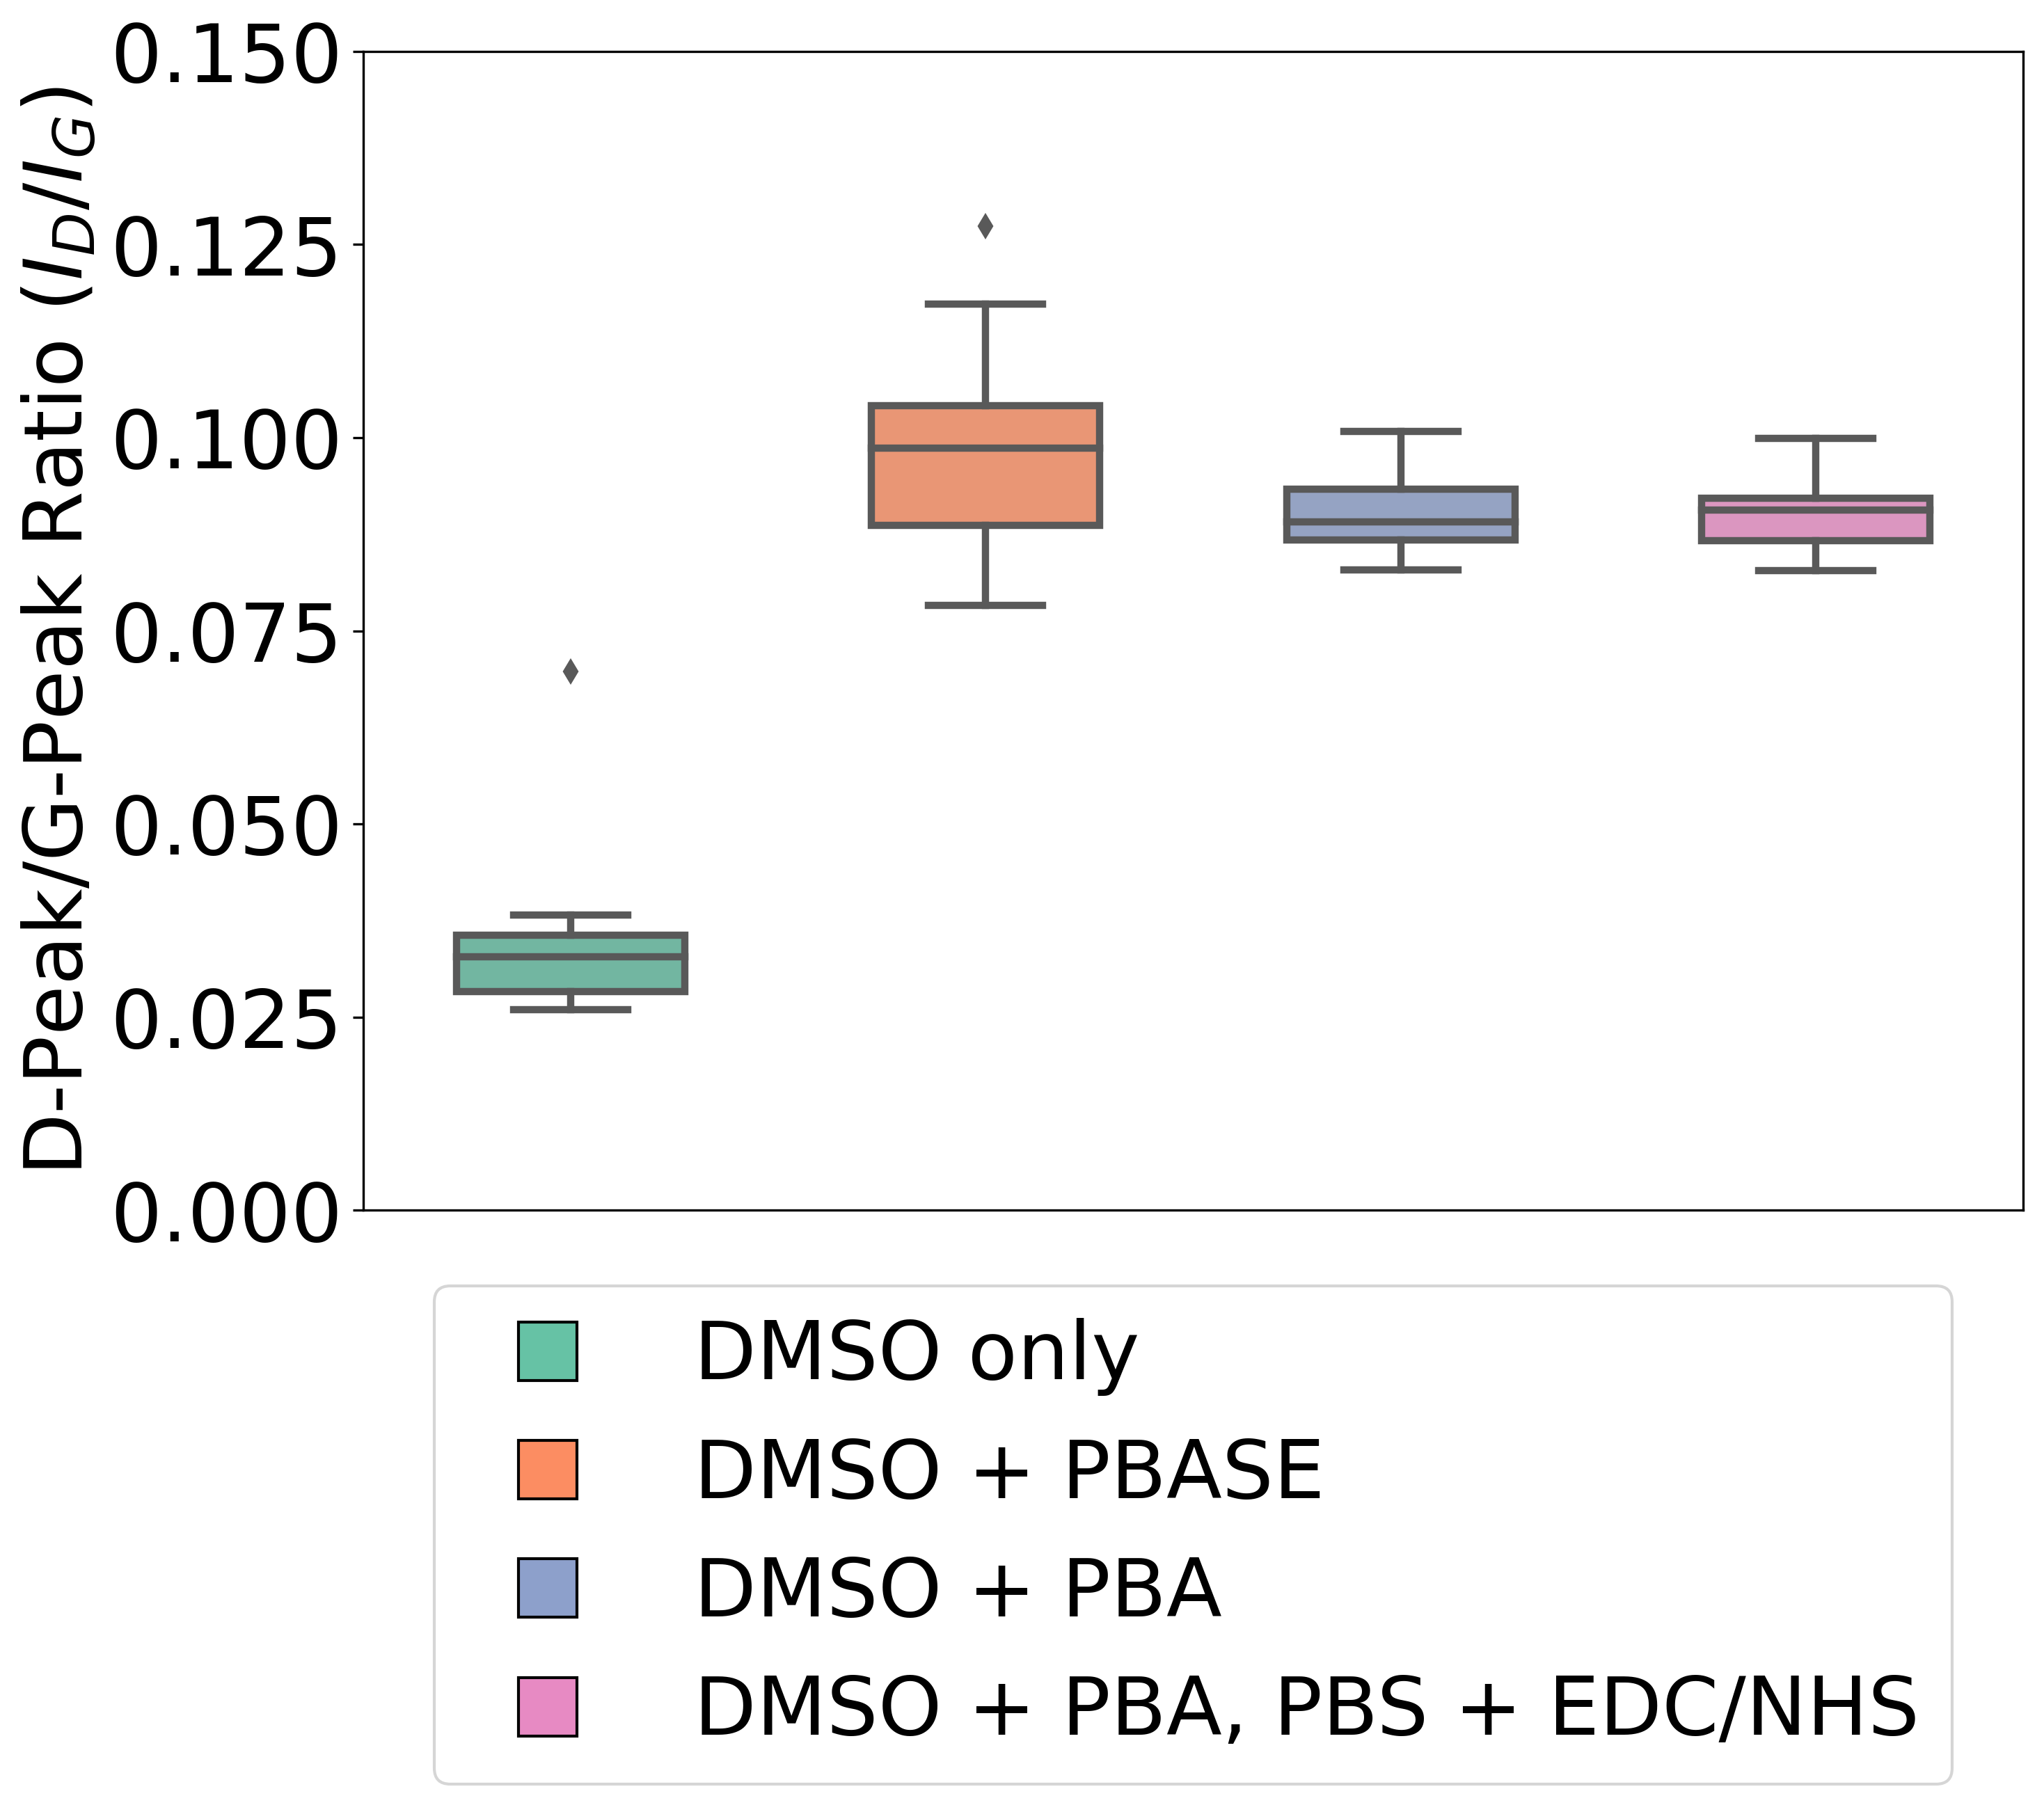
\includegraphics{figures/ch6/comparison_raman.png}

}

\caption{\label{fig-linker-raman}This box plot shows the distribution of
D-band peak to G\(^+\)-band peak ratio, I\(_D\)/I\(_G\), across nine
locations for a selection of chemically-modified carbon nanotube films.
The D-band and G-band intensities for all samples were first normalised
to the intensity peak corresponding to the silicon dioxide substrate.}

\end{figure}

Raman spectroscopy was used to verify the attachment of PBA to a carbon
nanotube network film with a silicon dioxide substrate in the manner
outlined in \textbf{?@sec-raman-characterisation}. As highly-bundled
devices were found to have less defects present prior to modification,
as discussed in \textbf{?@sec-pristine-raman}, solvent-deposited films
were used for the verification of pyrene attachment to prevent the
initial presence of defects influencing the analysis. Droplets of DMSO
solution were placed on three (solvent-deposited) carbon nanotube films
taken from the same wafer. The DMSO solution on one film contained 5 mM
PBA, the solution on another film contained 5 mM PBASE, and the DMSO on
the final film contained no linker molecule. After incubation for 1
hour, films were rinsed for 15 s with DMSO, then for 15 s with IPA to
remove excess DMSO while avoiding hydrolysis of the PBASE. After the
first set of Raman spectra was taken, the film initially exposed to PBA
was further exposed to a solution of 20 mM EDC and 40 mM NHS in 1XPBS
electrolyte for 30 minutes, and a second set of Raman spectra was taken
for this film. As in \textbf{?@sec-pristine-raman}, two spectra taken at
each position were processed according to
Section~\ref{sec-raman-analysis}, and the silicon dioxide reference peak
measured in the wavenumber range 100 cm\(^{-1}\) \(-\) 650 cm\(^{-1}\)
was used to normalise the D-band and G-band peaks from the wavenumber
range 1300 cm\(^{-1}\) \(-\) 1650 cm\(^{-1}\). The ratio between the
average intensity of the D-peak and the G\(^+\)-peak at each position
was calculated, and the distribution of ratio values corresponding to
each modified film is shown in Figure~\ref{fig-linker-raman}.

\begin{figure}

\begin{minipage}[t]{0.50\linewidth}

{\centering 

\raisebox{-\height}{

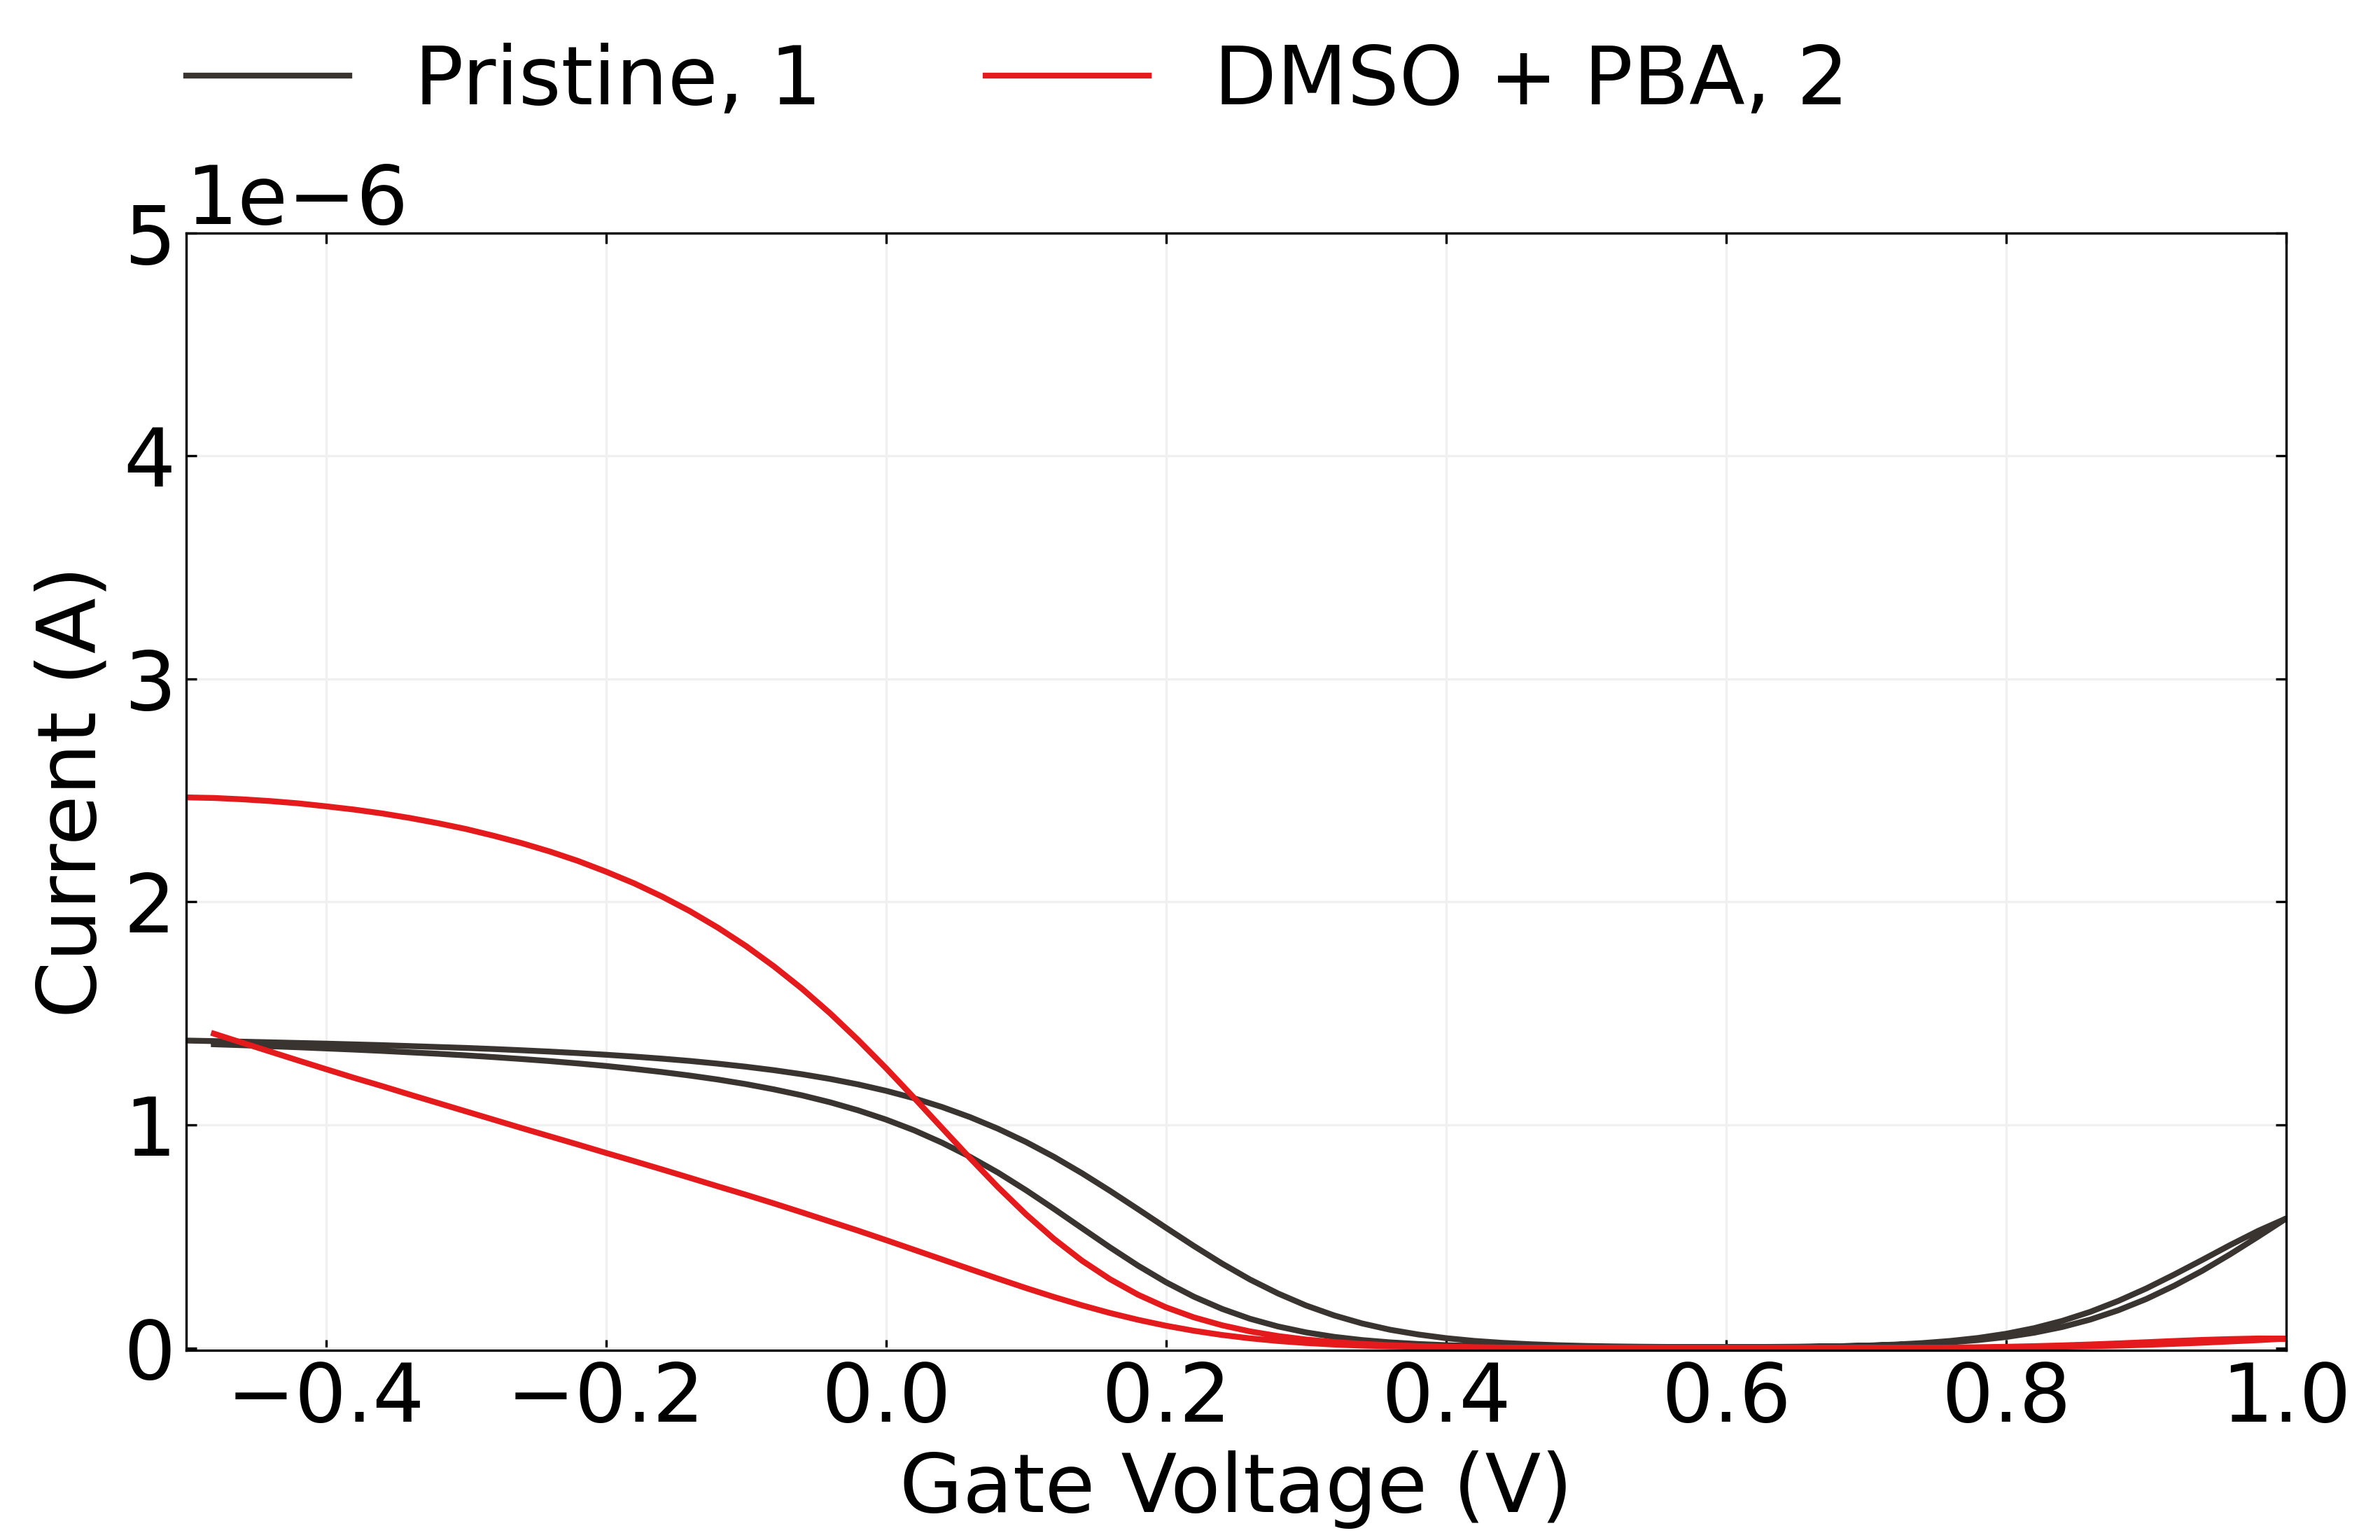
\includegraphics{figures/ch6/NTQ24C10_ch3_comparison_1.png}

}

}

\subcaption{\label{fig-pba-threshold-shift}}
\end{minipage}%
%
\begin{minipage}[t]{0.50\linewidth}

{\centering 

\raisebox{-\height}{

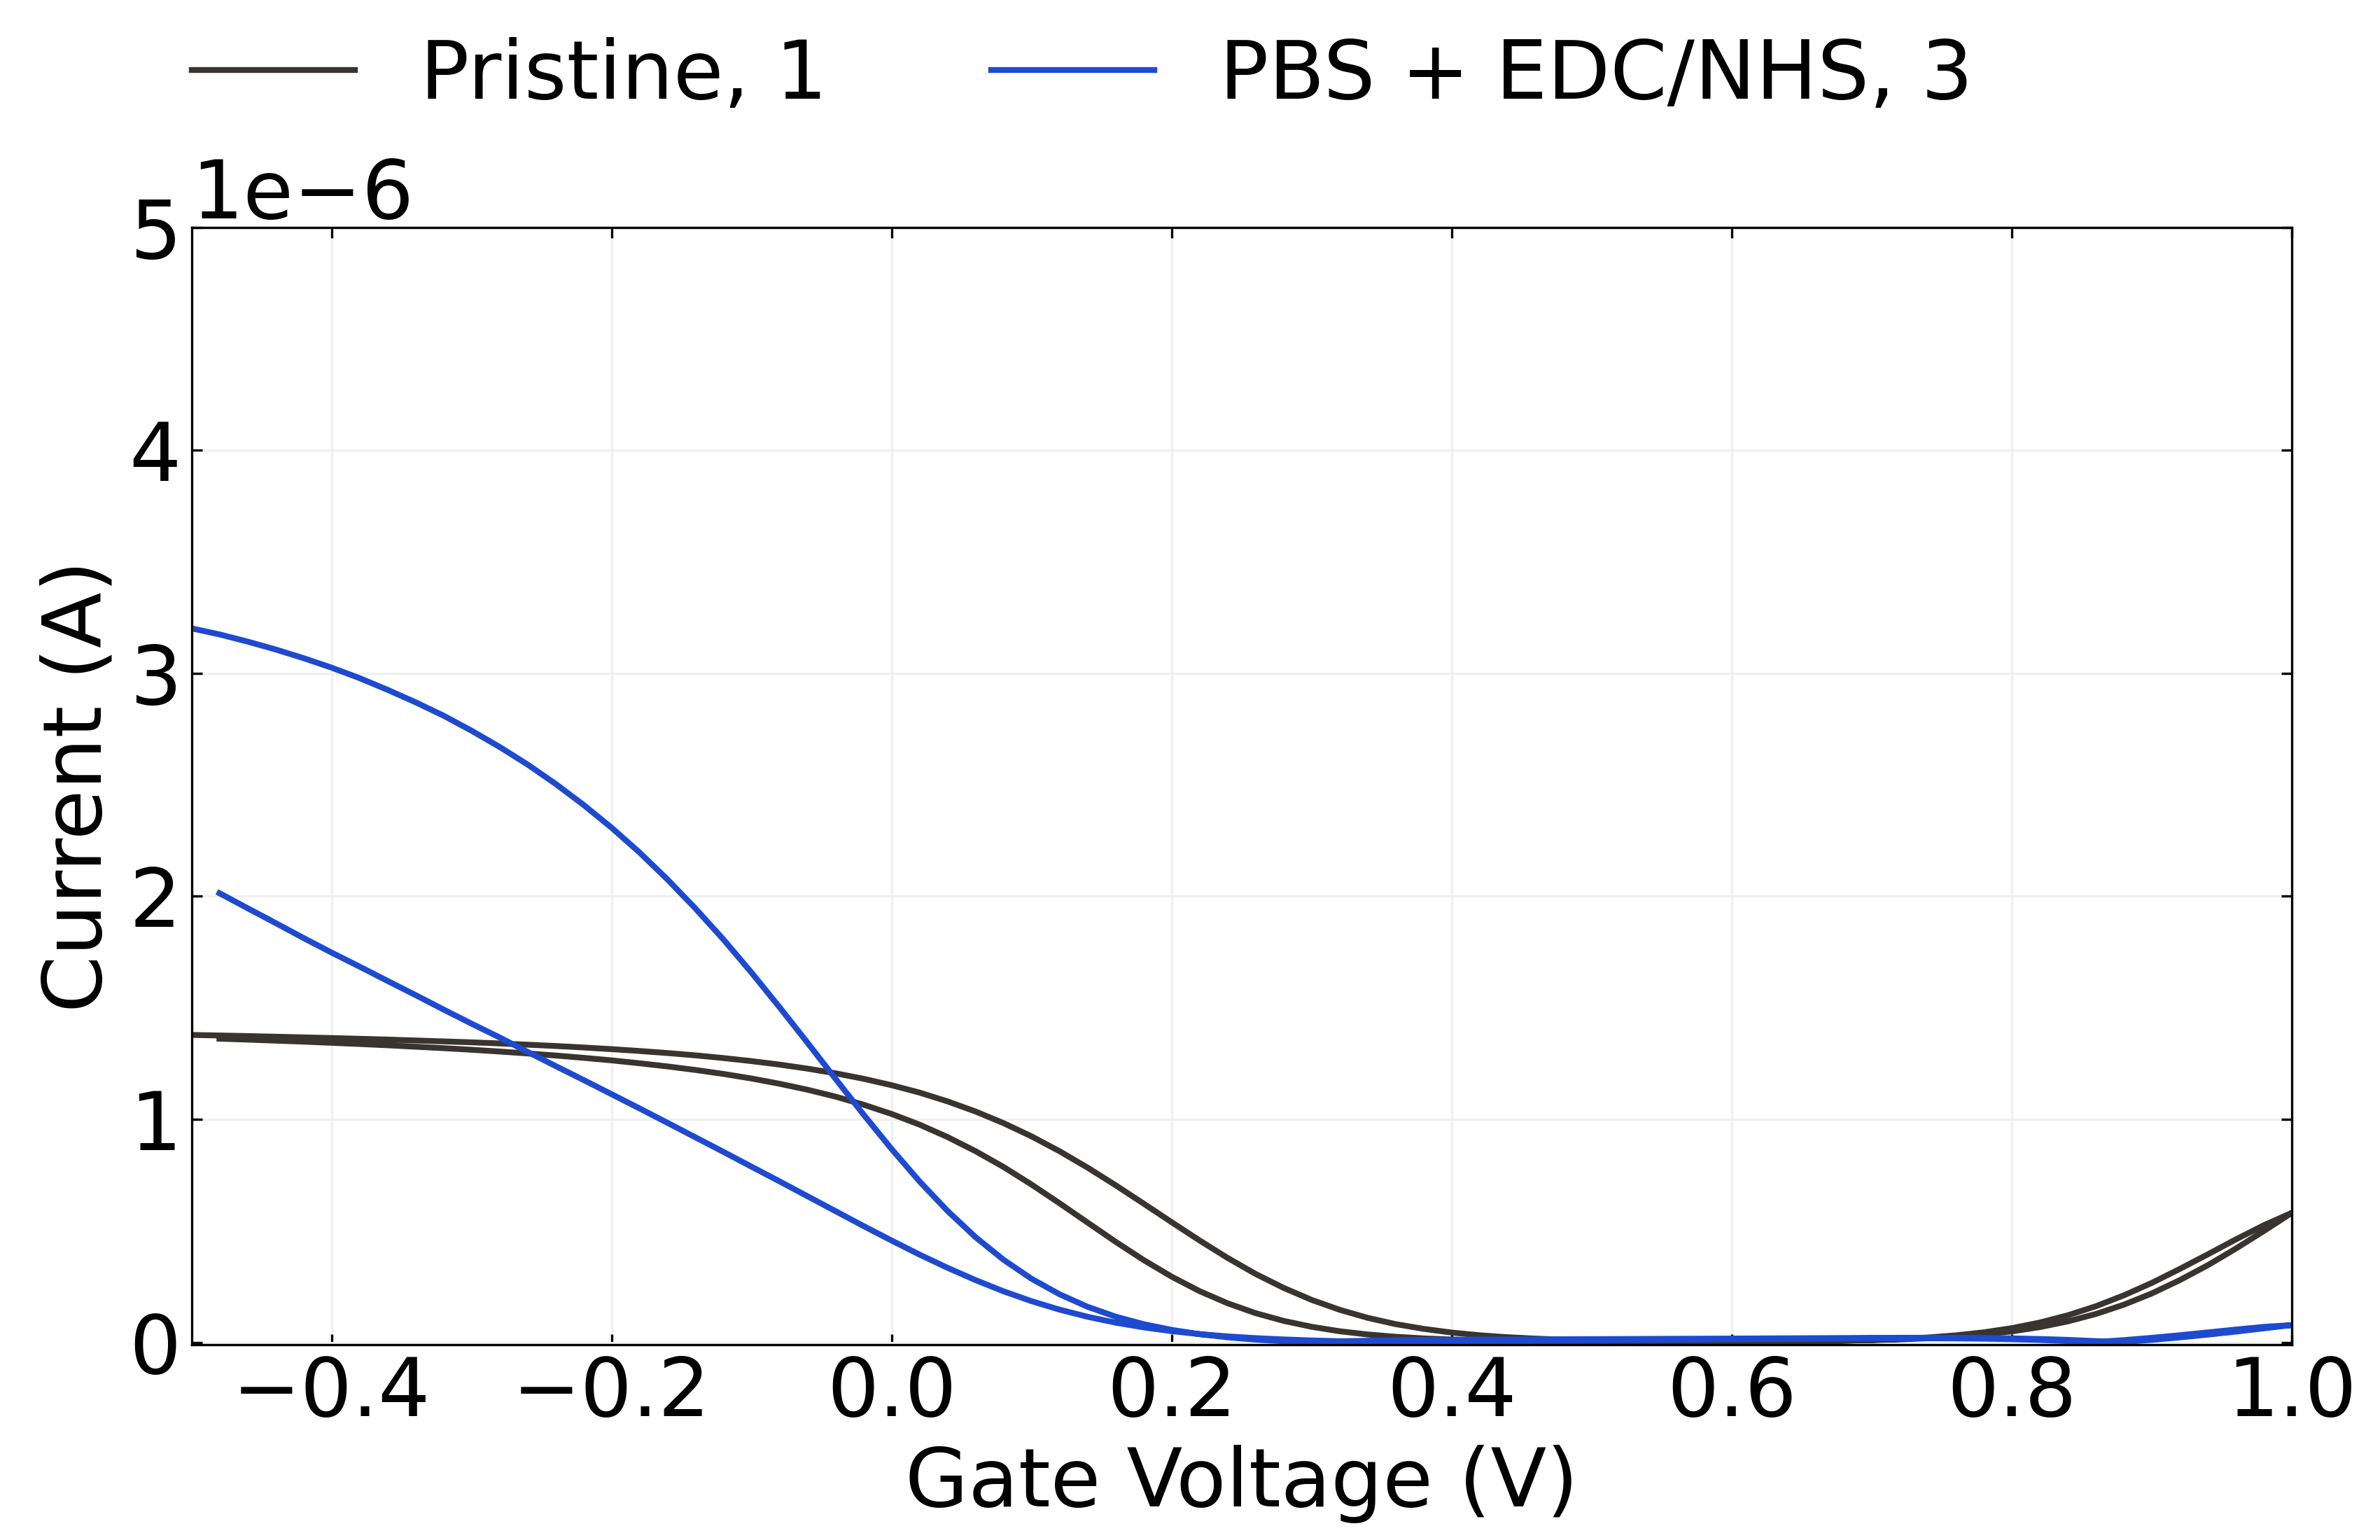
\includegraphics{figures/ch6/NTQ24C10_ch3_comparison_2.png}

}

}

\subcaption{\label{fig-edc-nhs-threshold-shift}}
\end{minipage}%
\newline
\begin{minipage}[t]{0.50\linewidth}

{\centering 

\raisebox{-\height}{

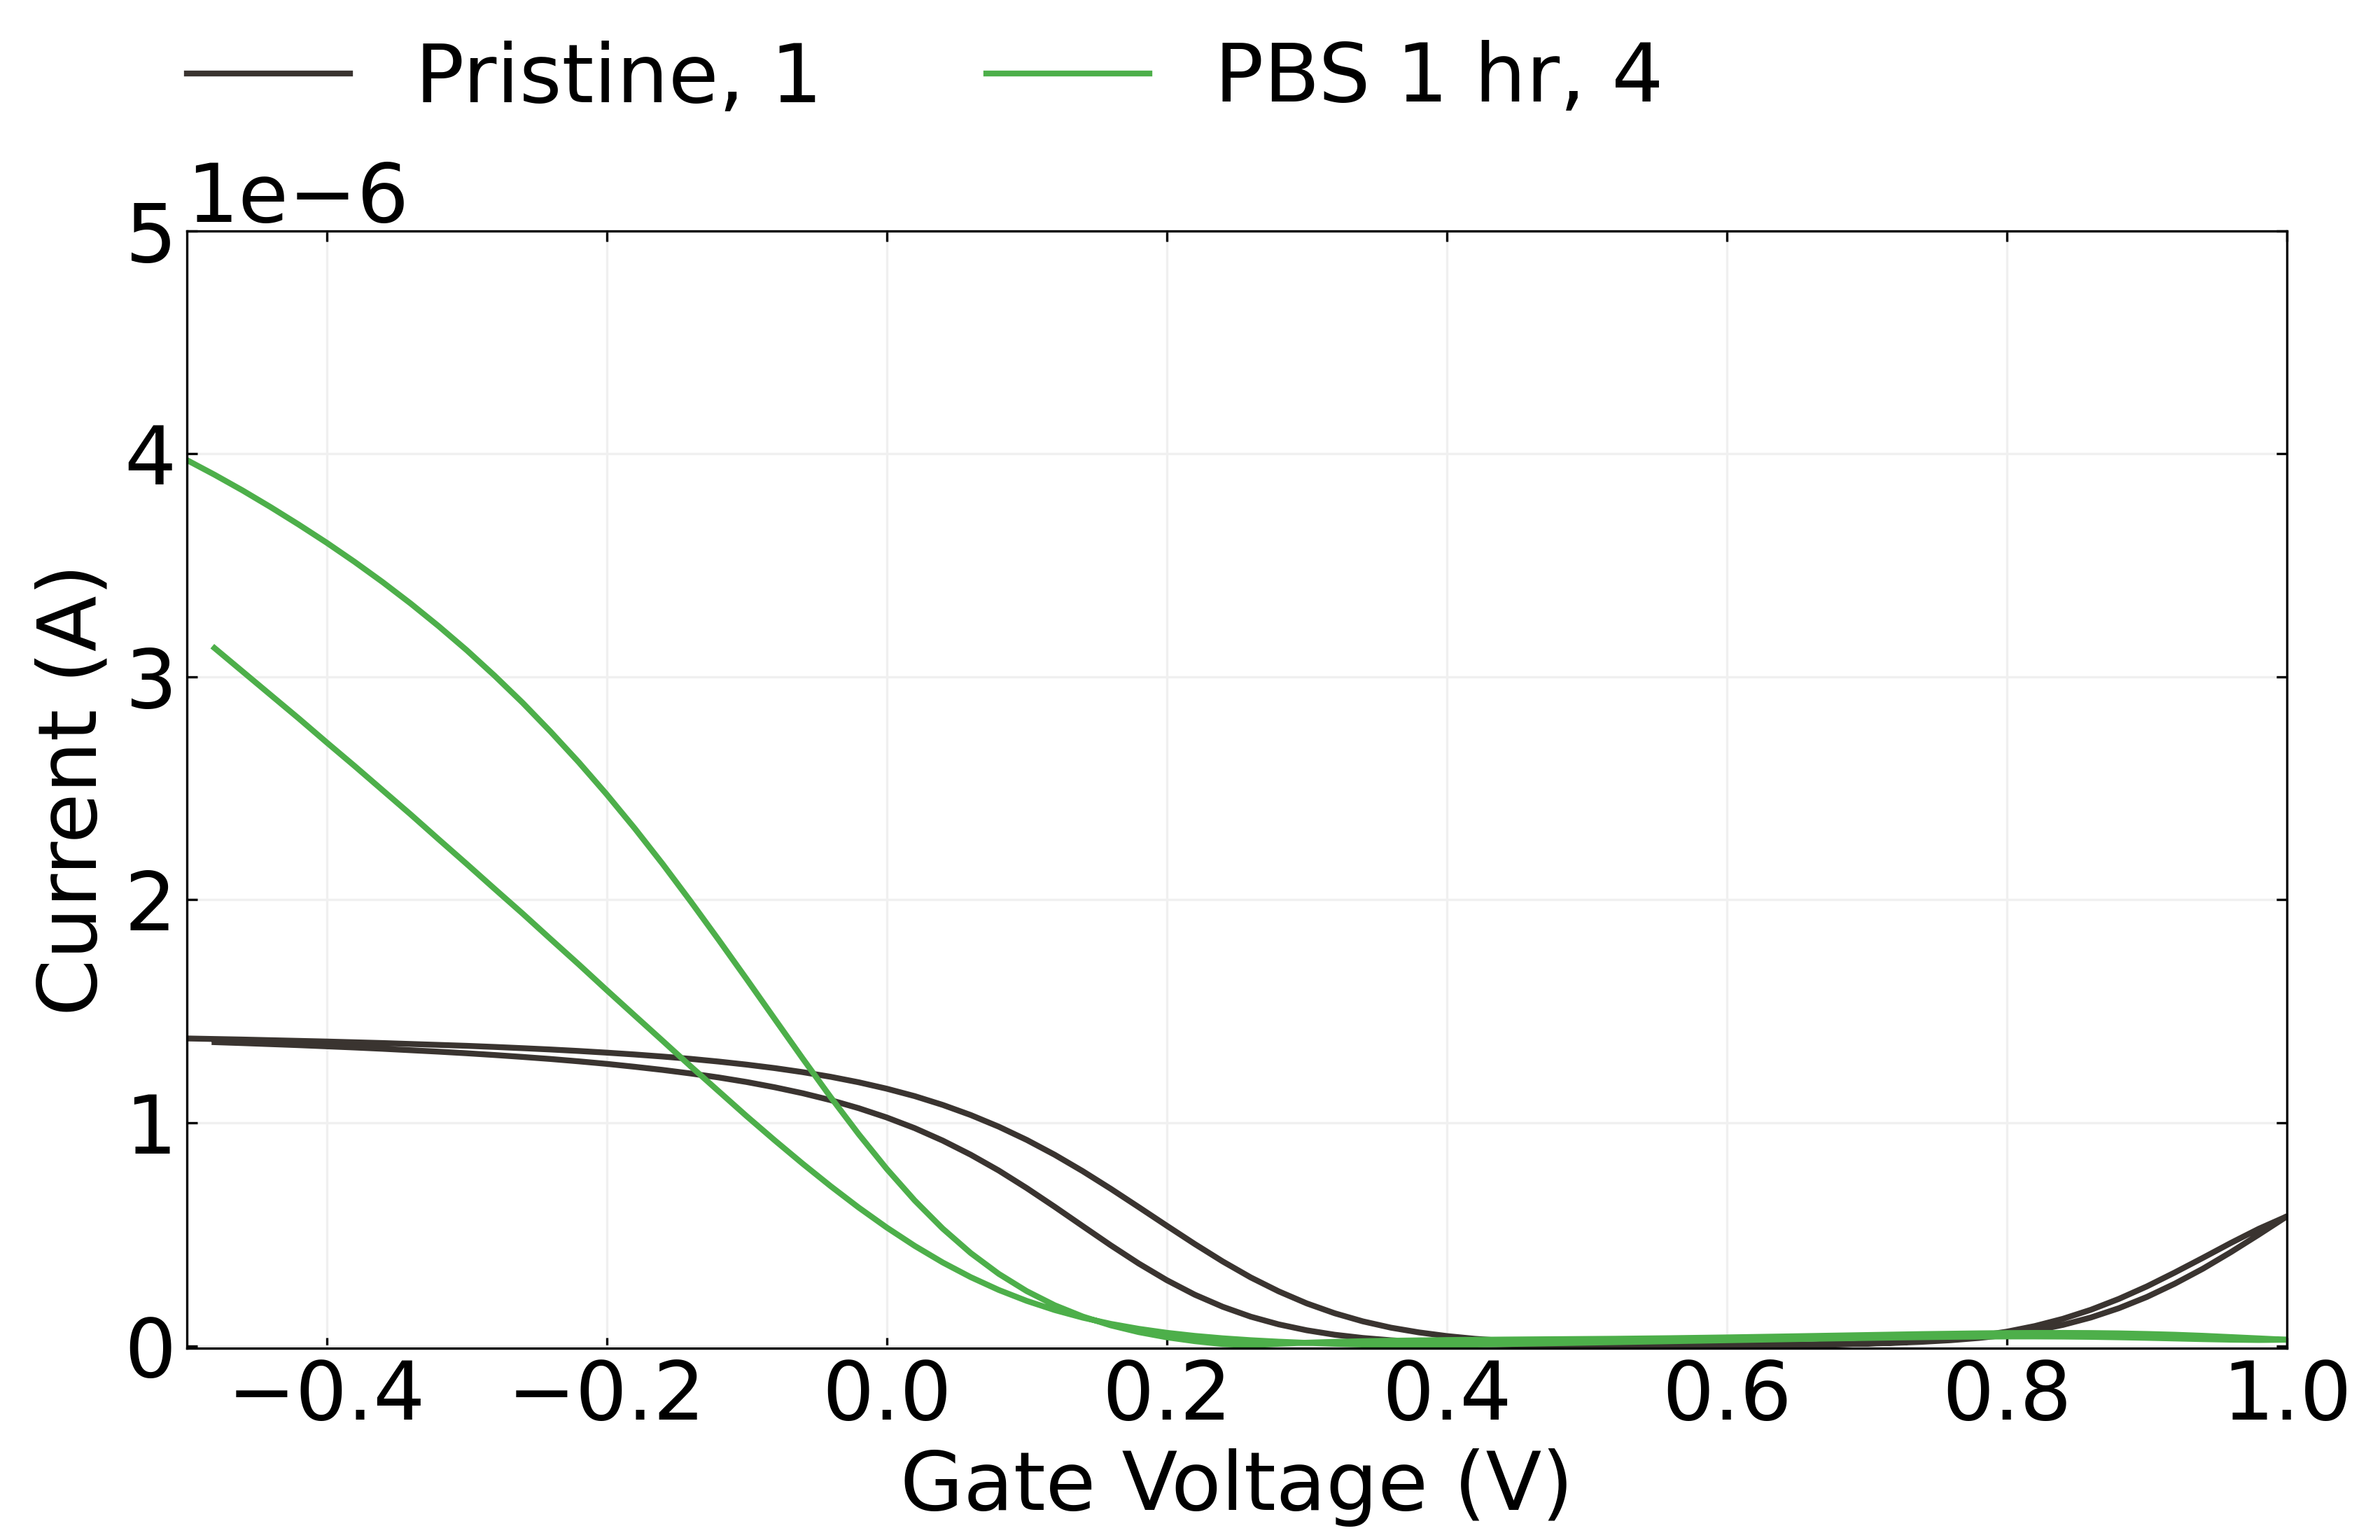
\includegraphics{figures/ch6/NTQ24C10_ch3_comparison_3.png}

}

}

\subcaption{\label{fig-rinse-threshold-shift}}
\end{minipage}%
%
\begin{minipage}[t]{0.50\linewidth}

{\centering 

\raisebox{-\height}{

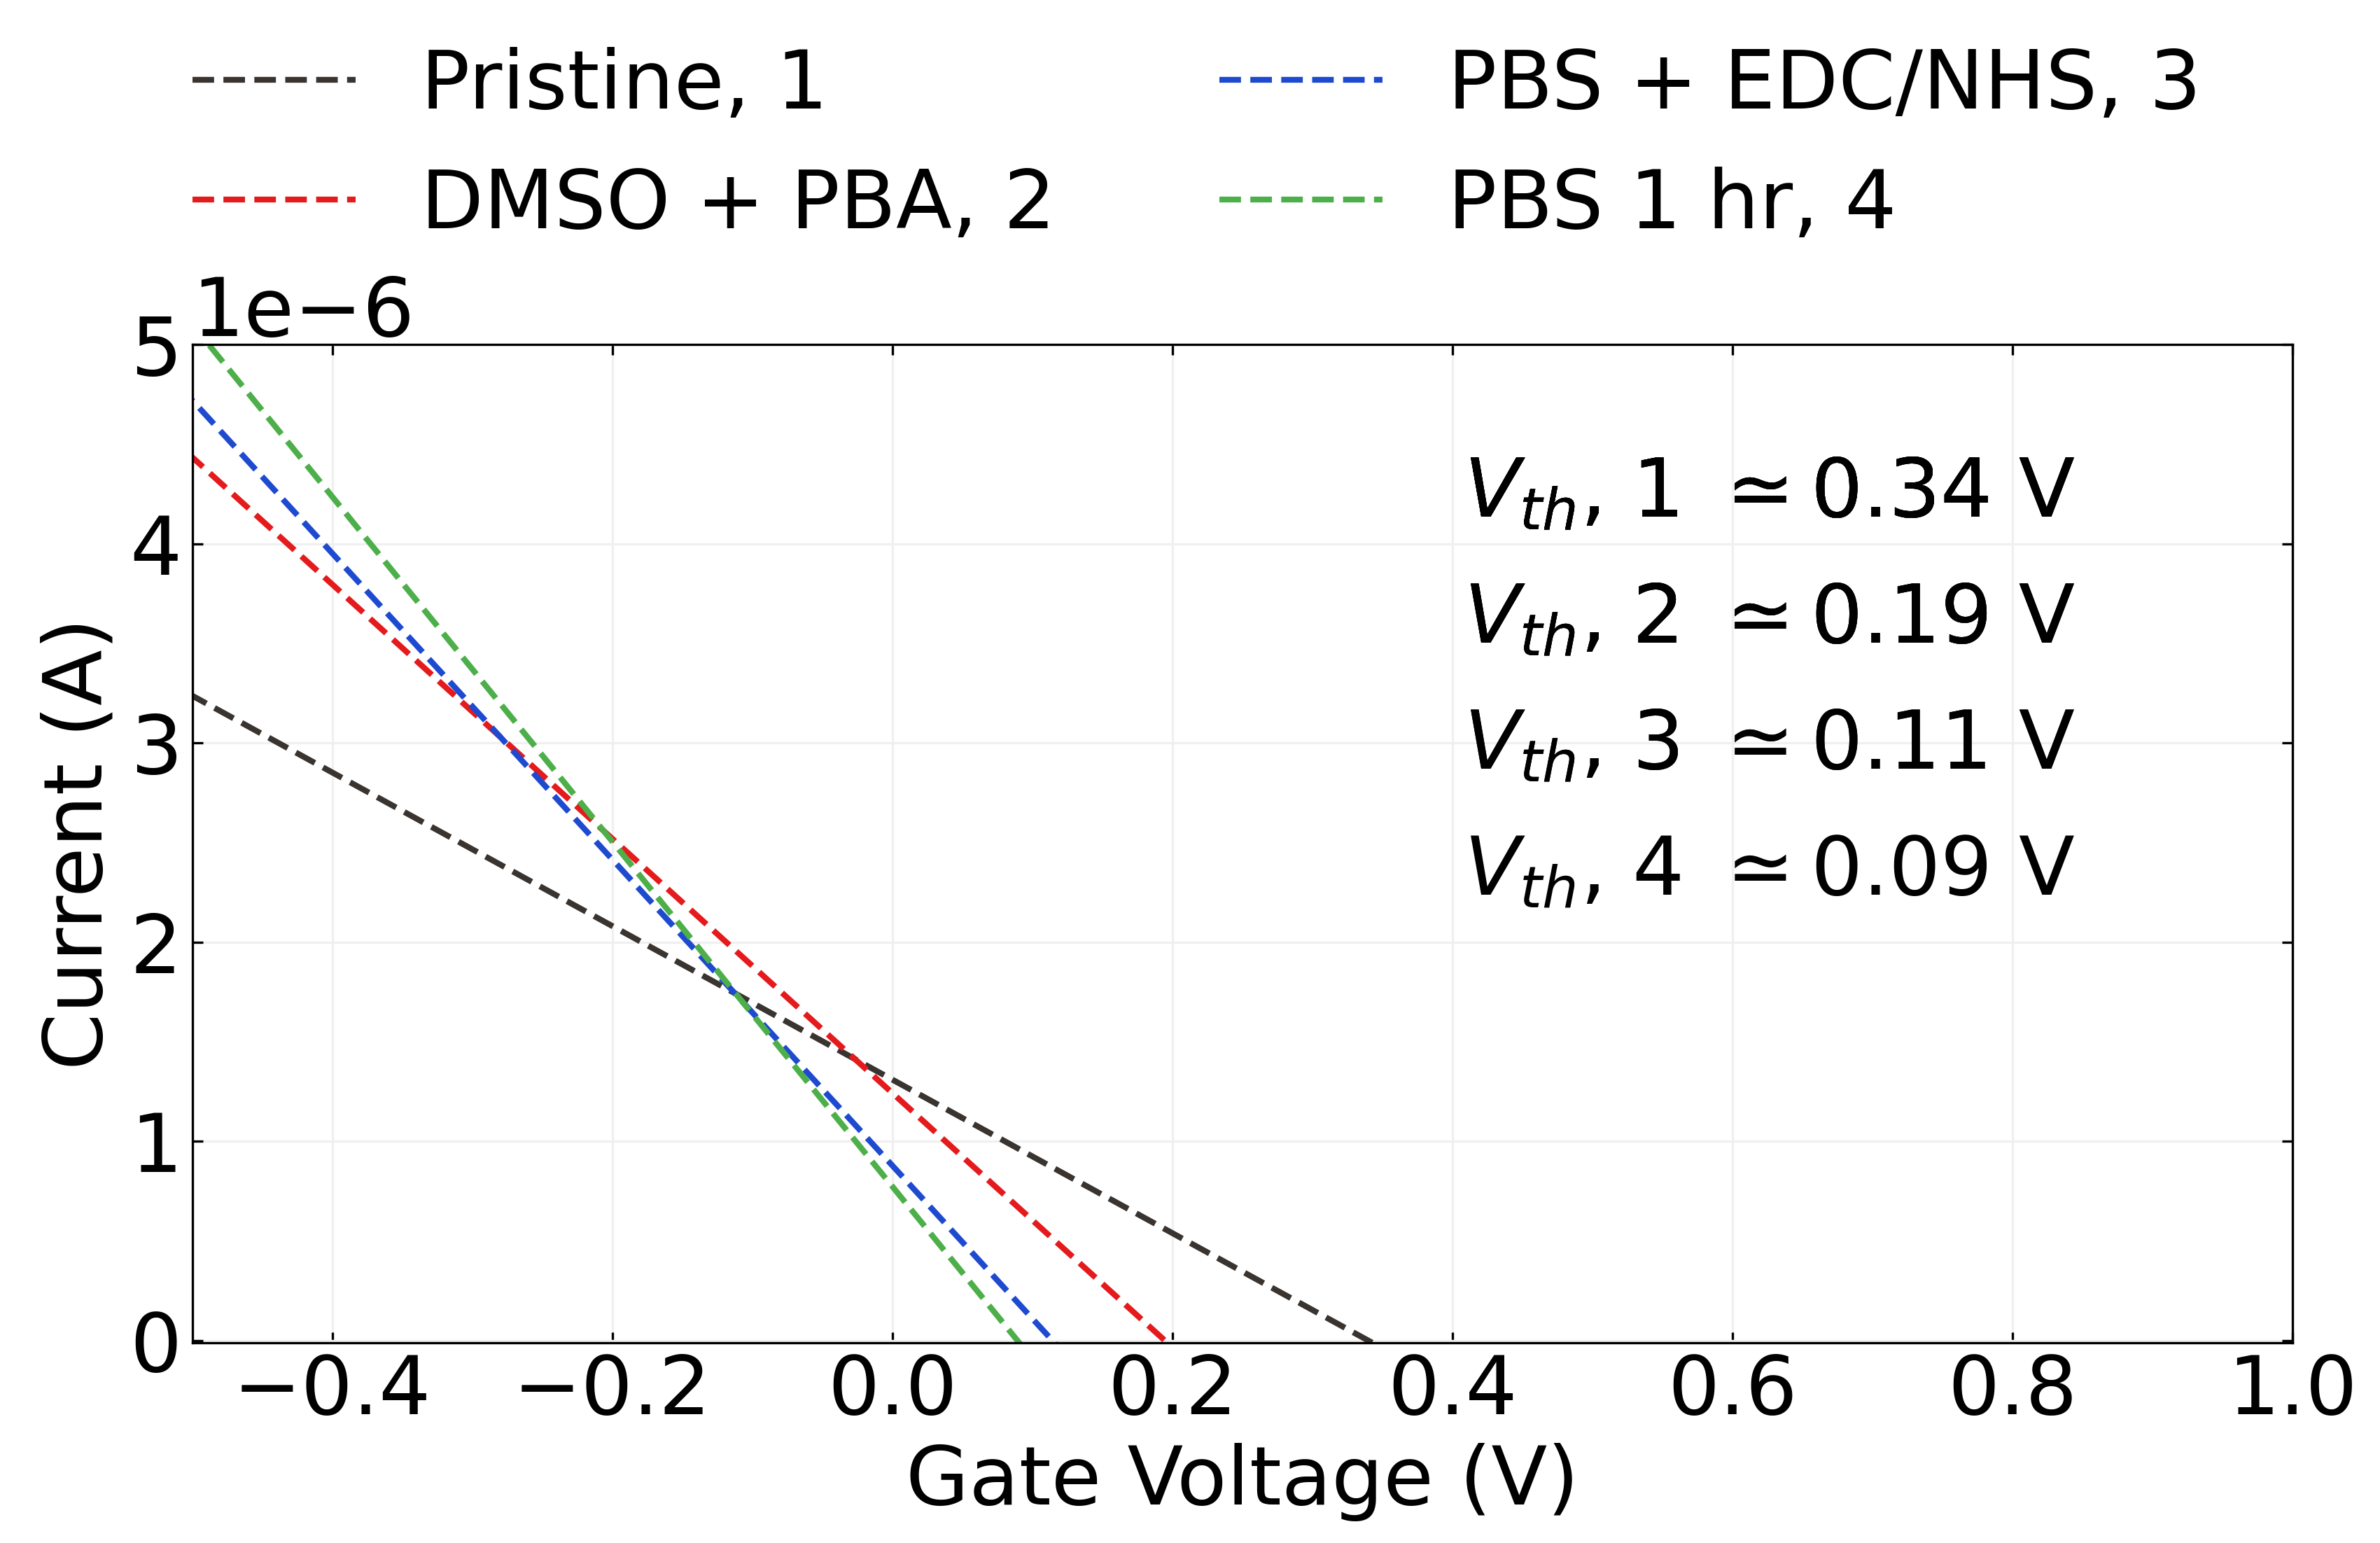
\includegraphics{figures/ch6/NTQ24C10_ch3_comparison_4.png}

}

}

\subcaption{\label{fig-pba-threshold-shift-comparison}}
\end{minipage}%

\caption{\label{fig-pba-functionalisation-threshold-shift}Electrical
transfer characteristics of a carbon nanotube transistor before
functionalisation alongside the transfer characteristics (a) after being
submerged in DMSO containing 5 mM PBA for 1 hour in red, (b) after being
submerged in 1XPBS containing 20 mM EDC and 40 mM NHS for 30 min in
blue, and (c) after being submerged in fresh 1XPBS for 1 hour in green.
The linear fits to each characteristic curve are shown in (d) as dashed
lines, alongside the threshold voltages calculated by finding the
intercept of each fit.}

\end{figure}

There is a \(\sim 3 \times\) increase in the intensity ratio
I\(_D\)/I\(_G\) for both the films modified with PBASE and PBA compared
to the film which was only exposed to DMSO. Previous works have found
that a change in the intensity ratio indicates successful
\(\pi\)-stacking on the carbon nanotube surface, as it indicates surface
modification of the carbon nanotubes has occurred
\autocite{Wei2010,Lan2013}. Wei \emph{et al.} \autocite{Wei2010} found
functionalisation with PBASE altered the ratio by a factor of
\(\sim 1.5 \times\), while Lan \emph{et al.} \autocite{Lan2013} found
that functionalisation with PBA altered the ratio by a factor of
\(\sim 0.8 \times\). The reason for the large difference between results
is not immediately clear, but may result from the significant
differences in the pristine composition and morphology of carbon
nanotube networks used in each publication, and differences in the
functionalisation method used. Across all scan locations in
\textbf{?@fig-raman-comparison}, the value found for I\(_D\)/I\(_G\) is
consistently \(\sim 0.095\) for both PBA and PBASE. Furthermore,
subsequent Raman measurements of the PBA-modified film after further
functionalisation with EDC/NHS do not show a significant change in
I\(_D\)/I\(_G\). These results indicate that presence of the NHS ester
has little effect on the Raman shift. It should be clarified that Raman
spectroscopy cannot be used to distinguish between the presence of PBA
and PBASE on the device surface. However, it is clear that
functionalisation of the carbon nanotube network with both the PBA and
PBASE has led to measurable \(pi\)-stacking between the network and the
pyrene group attached to each compound.

\hypertarget{electrical-characterisation-1}{%
\subsection{Electrical
Characterisation}\label{electrical-characterisation-1}}

Figure~\ref{fig-pba-functionalisation-threshold-shift} shows the
transfer characteristics of a carbon nanotube transistor channel at
various stages of a PBA/EDC functionalisation, where a excess of
N-hydroxysuccinimide (NHS) was added alongside EDC. A solvent-deposited
carbon nanotube film was used for the device. The PBA was dissolved in
DMSO, and the device channels were exposed to this solution for 1 hour.
The electrical change resulting from PBA exposure is shown in
Figure~\ref{fig-pba-threshold-shift}. The threshold shift with the
addition of 5 mM PBA in DMSO for 1 hour is equivalent to the shift seen
when only DMSO is added, \(\Delta\)V = -0.15 V. The lack of a
significant threshold shift directly attributable to the PBA is a result
of pyrene having a neutral charge state; any contributions from the
charged carboxyl group are screened from the carbon nanotube sidewalls
by surrounding water molecules \autocite{Lerner2012}. However, as in the
case of the addition of PBASE, there also appears to be an increase in
hole mobility, which may be due to the pyrene groups increasing
connectivity within the carbon nanotube network
\autocite{Murugathas2019b}.

Subsequently, the device was rinsed with 1XPBS and exposed to 20 mM EDC
and 40 mM NHS in 1XPBS electrolyte for 30 minutes.
Figure~\ref{fig-edc-nhs-threshold-shift} shows the change resulting from
subsequent EDC/NHS exposure. When EDC/NHS is added, a threshold shift of
\(\Delta\)V \(\sim\) -0.08 V was observed on multiple channels. The
exposure to EDC/NHS negatively shifts the transfer characteristic curve,
most likely due to the PBA present reacting to form positively-charged
\emph{O}-acylisourea esters and negatively gating the attached carbon
nanotube network \autocite{Heller2008,Hermanson2013-4}.
Figure~\ref{fig-rinse-threshold-shift} shows that this shift is not
significantly affected by further exposure of the channel to PBS. This
indicates that hydrolysis over the course of one hour is insufficient to
hydrolyse a significant proportion of the \emph{O}-acylisourea back to
PBA, as PBA is charge neutral. We therefore expect that the a
significant amount of \emph{O}-acylisourea remains active within this
time period and available for reaction with biomolecule amine groups.

\hypertarget{attachment-of-peglyated-pyrene-based-linkers}{%
\section{Attachment of PEGlyated Pyrene-Based
Linkers}\label{attachment-of-peglyated-pyrene-based-linkers}}

\hypertarget{sec-NTA-biotin-PEG}{%
\subsection{Pyrene-NTA, Pyrene-Biotin and
PEGylation}\label{sec-NTA-biotin-PEG}}

Through chemical coupling/conjugation, it is possible to replace the NHS
ester group on PBASE with other groups that can undergo binding
reactions with proteins. Unlike PBASE, these groups do not suffer the
drawback of being readily hydrolysed. For example, PBASE can be modified
with N\(\alpha\),N\(\alpha\)-Bis(carboxymethyl)-L-lysine hydrate (also
known as N-(5-Amino-1-carboxypentyl)iminodiacetic acid, AB-NTA) to
produce pyrene-nitrilotriacetic acid (pyrene-NTA). The attached NTA
group is able to chelate with metal ions such as Cu\(^{2+}\) or
Ni\(^{2+}\), which then can then coordinate with polyhistidine-tags
attached to a protein \autocite{Holzinger2011,Amano2016,Chang2017}. Use
of Cu\(^{2+}\) ions over Ni\(^{2+}\) gives stronger histidine bonding
and less non-specific adsorption \autocite{Chang2017}. Functionalisation
using the NTA-Ni\(^{2+}\) chemistry was successfully used to attach
mammalian odorant receptors to a single carbon nanotube for detection of
eugenol vapour in real-time \autocite{Goldsmith2011}. Pyrene-biotin
(pyrene butanol biotin ester) can also be produced for attaching avidin
or strepavidin \autocite{Holzinger2011}. As avidin and strepavidin are
tetrameric, they can be attached to both pyrene-biotin and biotinylated
avi-tagged proteins simultaneously via strong non-covalent bonding,
therefore linking the transducer and receptor
\autocite{Star2003a,Dundas2013,Hermanson2013-11,Fairhead2015}. As the
presence of his-tags and avi-tags on proteins can be readily controlled,
these methods offer improved specificity and directionality over the
traditional amide bonding seen earlier.

It is also possible to attach polyethylene glycol (PEG) chains to a
pyrene group and modify them with reactive groups such as NTA and biotin
to attach proteins in the manner outlined in the previous paragraph
\autocite{Hermanson2013-18,Meran2018}. Once modified with PEG, the water
solubility of pyrene linkers increases, making it possible to perform a
full functionalisation procedure exclusively in aqueous solution
\autocite{Hermanson2013-18}. By setting the length of the PEG chain, the
size of the linker molecule can be controlled - selection of a short
chain is important for ensuring attached receptors remain within the
Debye length of the transducer \autocite{Shkodra2021}. Functionalisation
of a graphene transducer with pyrene-PEG-biotin has previously been used
to bind streptavidin to a graphene field-effect transistor device
\autocite{Miki2019}. The PEGlyated linkers used in the following
sections were purchased pre-prepared. Pyrene-PEG-NTA (2 kDa) was
purchased from Nanocs, while pyrene-PEG-FITC (2 kDa, 10 kDa),
pyrene-PEG-rhodamine (3.4 kDa), mPEG-Pyrene (10 kDa) and
pyrene-PEG-biotin (10 kDa) were purchased from Creative PEGworks.

\hypertarget{sec-PPF-fluorescence-characterisation}{%
\subsection{Fluorescence Characterisation with
Pyrene-PEG-FITC}\label{sec-PPF-fluorescence-characterisation}}

\begin{figure}

\begin{minipage}[t]{0.47\linewidth}

{\centering 

\raisebox{-\height}{

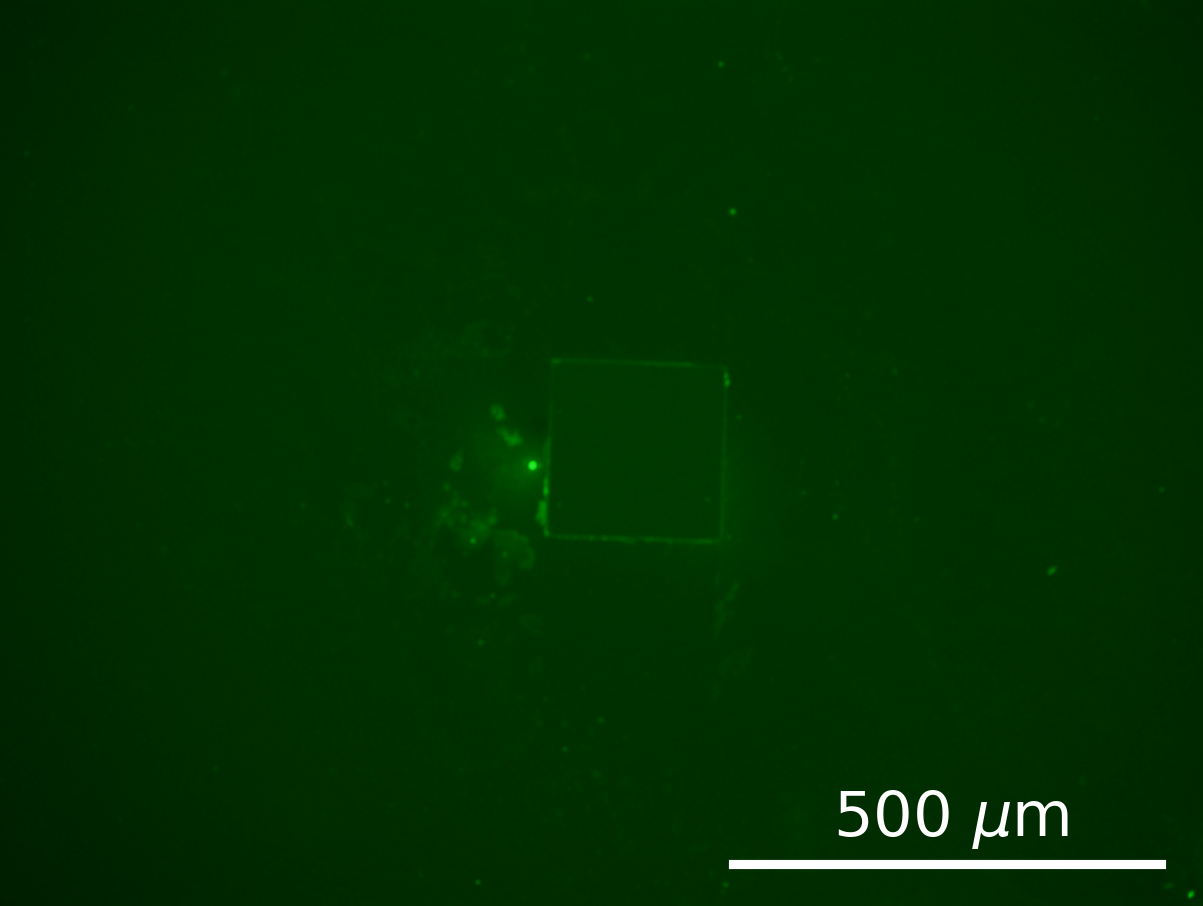
\includegraphics{figures/ch6/NGW8D1_FITC_6.5sexposure_10X_221121.png}

}

}

\subcaption{\label{fig-FITC}}
\end{minipage}%
%
\begin{minipage}[t]{0.05\linewidth}

{\centering 

~

}

\end{minipage}%
%
\begin{minipage}[t]{0.47\linewidth}

{\centering 

\raisebox{-\height}{

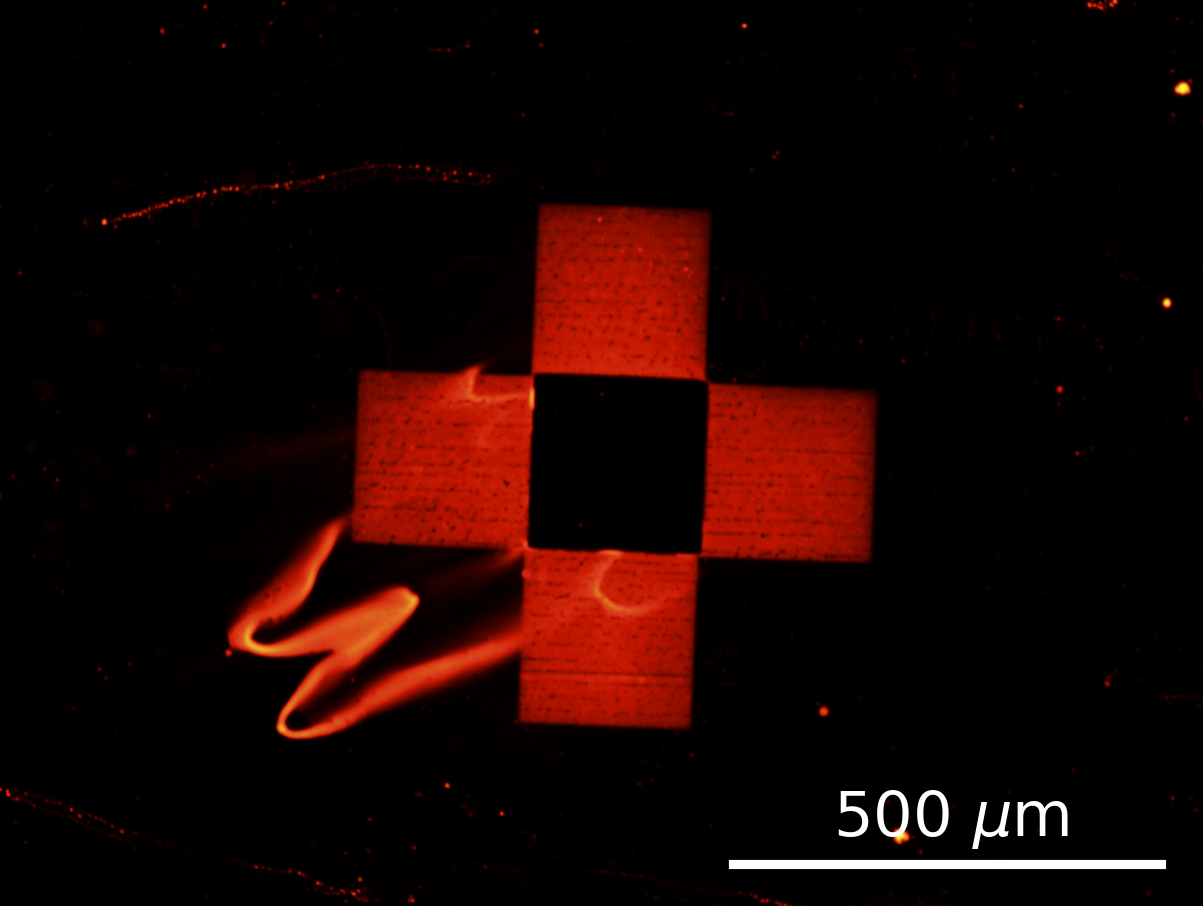
\includegraphics{figures/ch6/NGW8D4_rhodamineB_cornergraphene_221110.png}

}

}

\subcaption{\label{fig-rhodamine}}
\end{minipage}%

\caption{\label{fig-FITC-rhodamine-B}Four 200 \(\mu\)m \(\times\) 200
\(\mu\)m graphene squares modified with the dyes (a) fluorescein
isothiocyanate (FITC) and (b) Rhodamine B. No pyrene/PEG/pyrene-PEG was
attached to these dyes. In (a), an FITC filter and 6.5 s exposure time
was used, and in (b) a Texas Red filter and 1.4 s exposure time was
used.}

\end{figure}

Dye attachment was used to map the prescence of PEGlyated pyrene-based
linkers across a carbon nanotube or graphene surface with fluorescence
microscopy. Four 200 \(\mu\)m \(\times\) 200 \(\mu\)m graphene squares
were incubated in two commonly used and easily obtained dyes,
fluorescein isothiocyanate (FITC) and Rhodamine B, to test whether the
dyes themselves bond to graphene.

The functionalisation of graphene devices with fluorescent dye was
performed using the following steps:

\begin{enumerate}
\def\labelenumi{\arabic{enumi}.}
\item
  1 mM dye (FITC or Rhodamine B) prepared in PBS solution by vortex
  mixing for 10-15 minutes.
\item
  Graphene on silicon dioxide substrate rinsed with acetone and IPA,
  then nitrogen dried, and then treated with 300 mTorr 5W oxygen plasma
  for 15 s (see Section~\ref{sec-hydrophobicity}).
\item
  Immediately (in less than 1 min) place a 20 \(\mu\)L droplet of dye
  solution onto the substrate surface, near wet tecwipes to keep
  droplets humidified, covered with a glass container. Leave for 20
  minutes.
\item
  After 20 minutes, substrate rinsed in PBS for 30 s.
\item
  Substrate rinsed with m-CNT dispersion solution for 5 minutes at
  70\(^\circ\)C with a pipette, then rinsed with DI water, ethanol,
  acetone, IPA and nitrogen dried (see
  Section~\ref{sec-pyrene-interactions}).
\end{enumerate}

The results of this test are shown in Figure~\ref{fig-FITC-rhodamine-B}.
There is a much stronger contrast between the graphene squares and the
background after functionalisation with Rhodamine B, showing a clear,
specific interaction between Rhodamine B and graphene. It has previously
been determined that the benzene rings of rhodamine \(\pi\)-stack with
carbon rings \autocite{Tang2012}. Rhodamine B could therefore not be
used as a fluorescent marker to check for attachment of our linker
molecules. However, as fluorescein isothiocyanate did not show
significant interaction with the graphene, this marker was subsequently
used for fluorescent mapping linker attachment.
Figure~\ref{fig-PPF-concs} shows various concentrations of
pyrene-PEG-FITC dissolved in 1XPBS, which is used for fluorescence
characterisation in this section.

Both SU8 and AZ\(^\circledR\) 1518 photoresist were found to fluoresce,
which is due to their photoactive component \autocite{Pai2007}. This
passive fluorescence was found to drown out fluorescence from a
dye-functionalised device channel, and so photoresist encapsulated
devices were not used for fluorescence imaging. A different type of
encapsulation could potentially be used to verify linker attachment with
fluorescence after a device has been encapsulated. These alternative
encapsulation methods for use with fluorescence microscopy are discussed
in \textbf{?@sec-future-work}.

\begin{figure}

{\centering 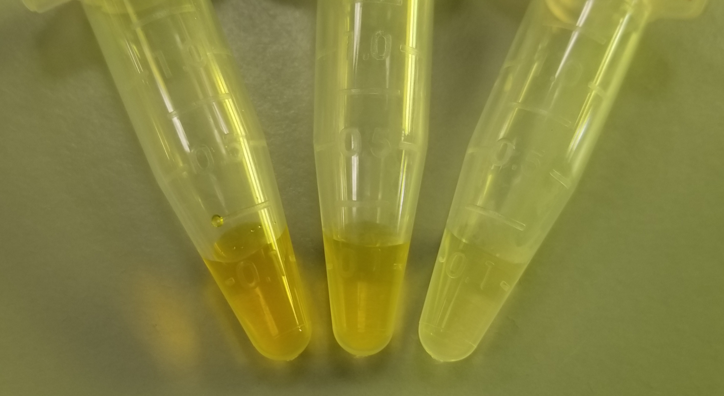
\includegraphics[width=0.45\textwidth,height=\textheight]{figures/ch6/PPF_vials.png}

}

\caption{\label{fig-PPF-concs}Microcentrifuge tubes containing various
concentrations of 10 kDa pyrene-PEG-FITC in solution (1 mM, 0.1 mM and
0.01 mM left to right)}

\end{figure}

The functionalisation of graphene devices with pyrene-PEG-FITC was
performed as follows:

\begin{enumerate}
\def\labelenumi{\arabic{enumi}.}
\item
  1 mM pyrene-PEG-FITC was prepared in ethanol by sonication for 1
  minute then vortex mixing for 10-15 minutes, to fully dissolve the
  pyrene-PEG-FITC (Note: pyrene-PEG-FITC is stored frozen, should be
  defrosted under vacuum 15 minutes before use).
\item
  Unencapsulated device was rinsed with acetone and IPA, then nitrogen
  dried.
\item
  The device was then fully submerged in pyrene-PEG-FITC/ethanol
  solution for 20 minutes.
\item
  After 20 minutes, device was rinsed for 30 s with ethanol, then
  acetone, IPA and nitrogen dried.
\end{enumerate}

Fluorescence images of the unencapsulated graphene devices successfully
functionalised with pyrene-PEG-FITC (PPF), showing up bright green
against a dark background, are shown in Figure~\ref{fig-FITC-EtOH}. As
indicated by the labels, the darkest regions are the titanium-gold
electrodes, and the bright green region is the PPF functionalised
graphene channel. It is noticable that some variation in fluorescence is
seen between channels, indicating the quality of functionalisation may
vary across the channels of a device. Some of the difficulties
encountered when investigating functionalisation with pyrene-PEG-FITC
are discussed later in Section~\ref{sec-impediments}.

\begin{figure}

\begin{minipage}[t]{0.47\linewidth}

{\centering 

\raisebox{-\height}{

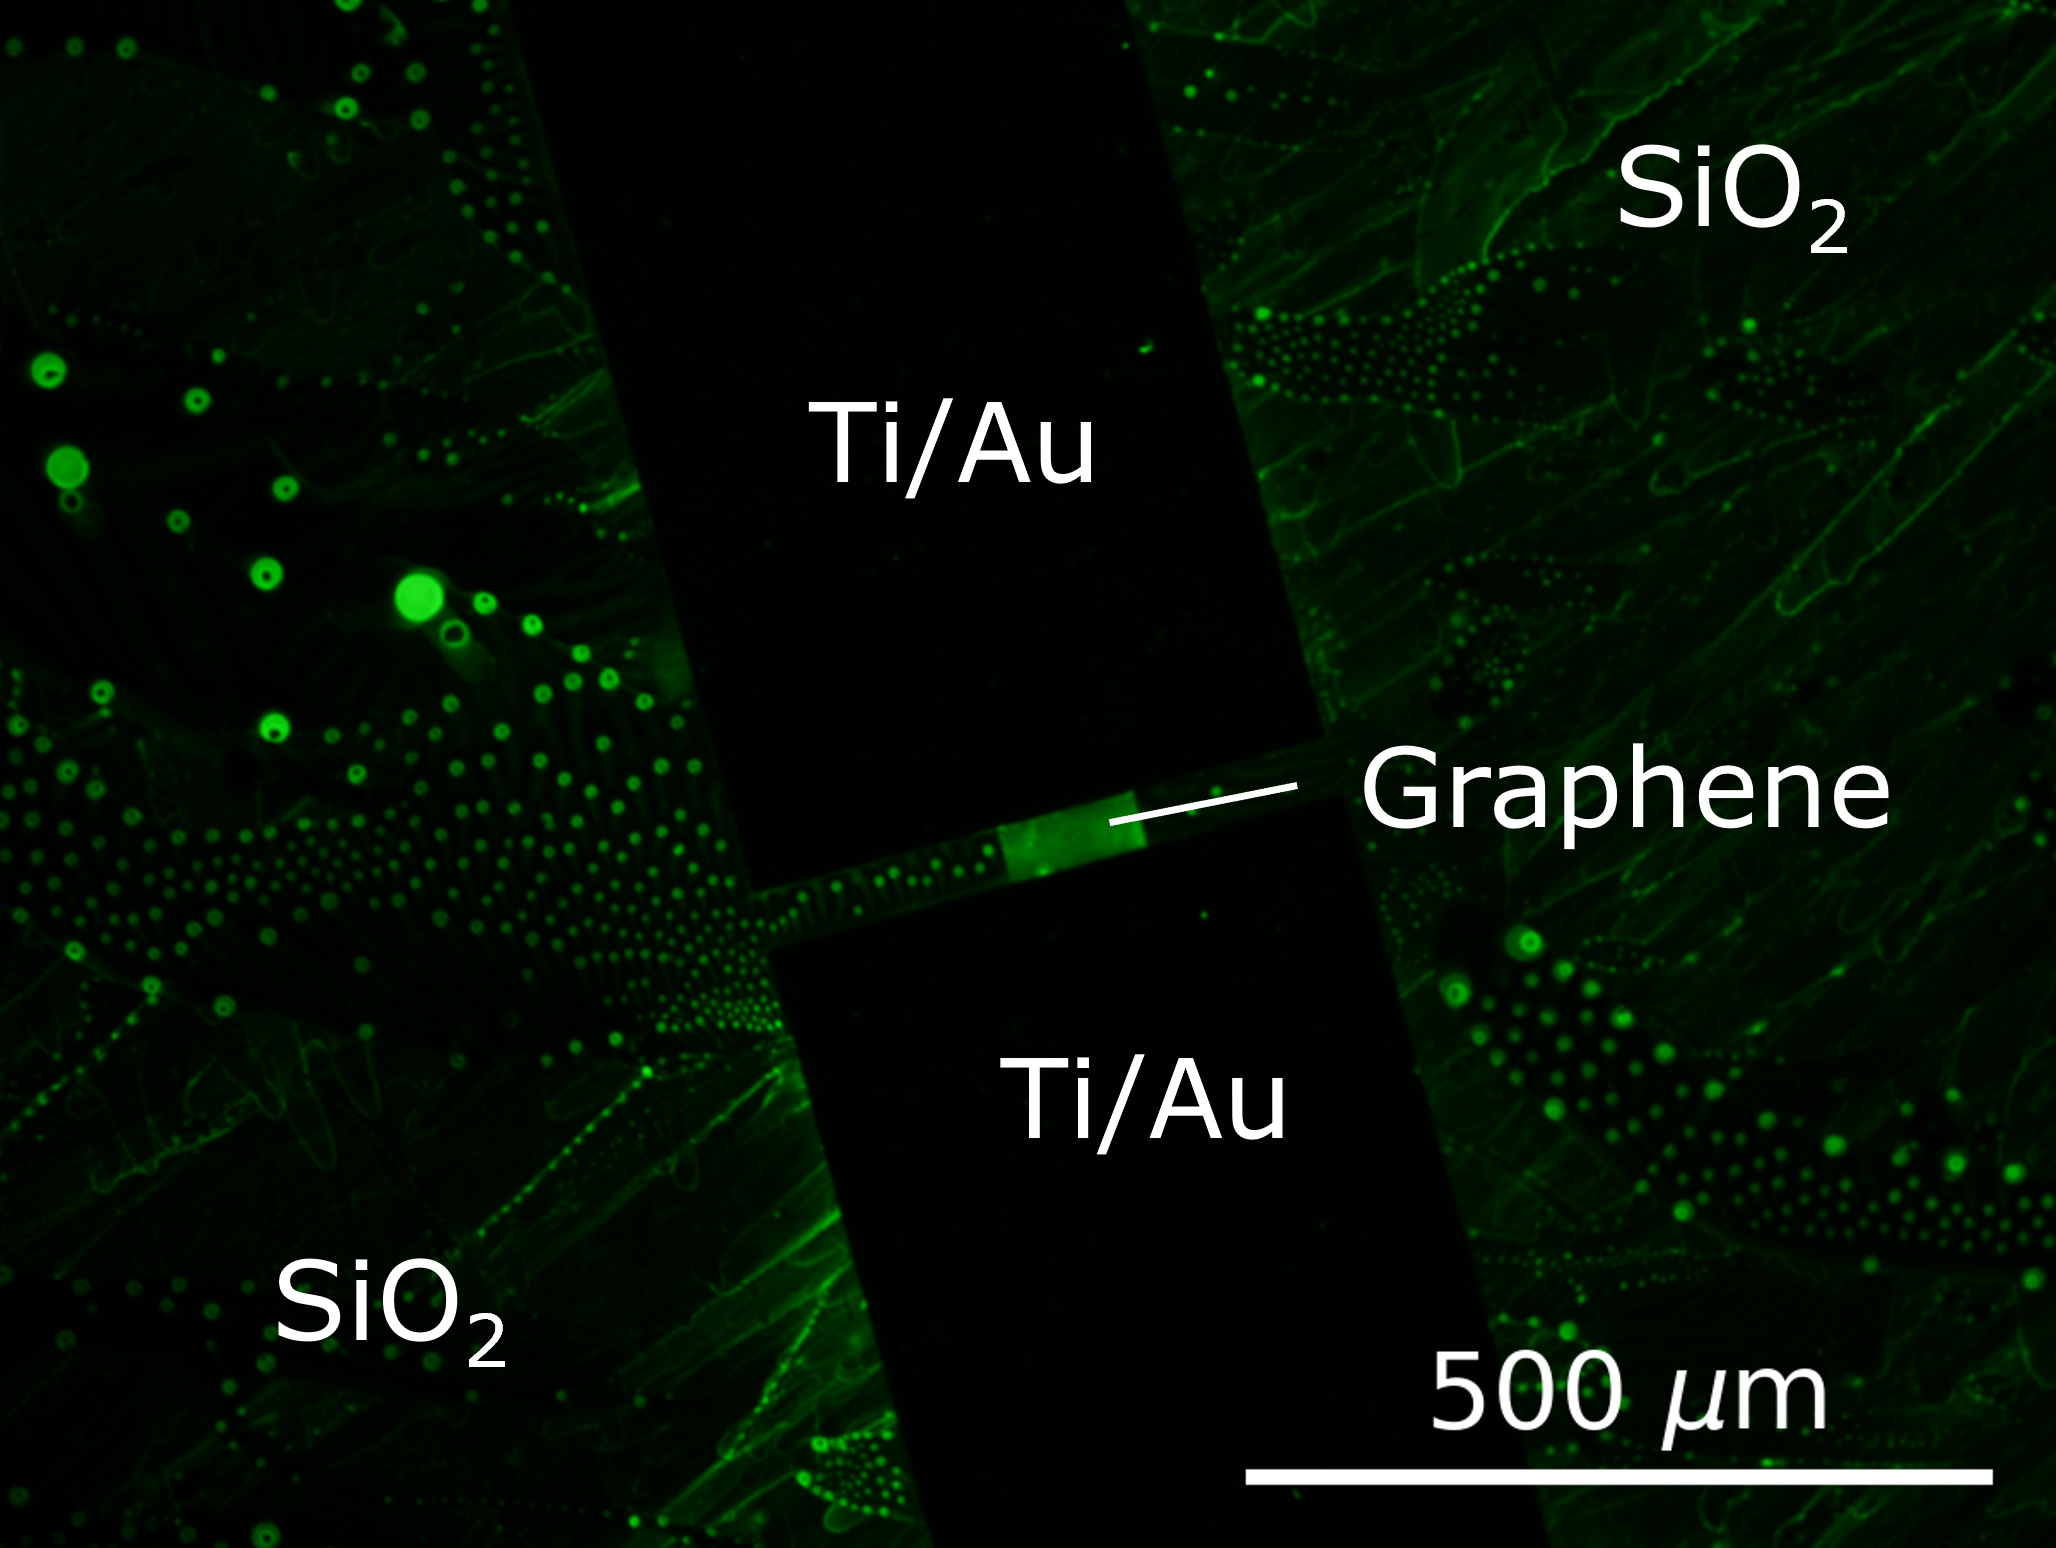
\includegraphics{figures/ch6/labelled_modified_noencap_1mMPPF_channel2_1sexposure_6.3X_highcontrast_221214.png}

}

}

\subcaption{\label{fig-FITC-EtOH-ch2}}
\end{minipage}%
%
\begin{minipage}[t]{0.05\linewidth}

{\centering 

~

}

\end{minipage}%
%
\begin{minipage}[t]{0.47\linewidth}

{\centering 

\raisebox{-\height}{

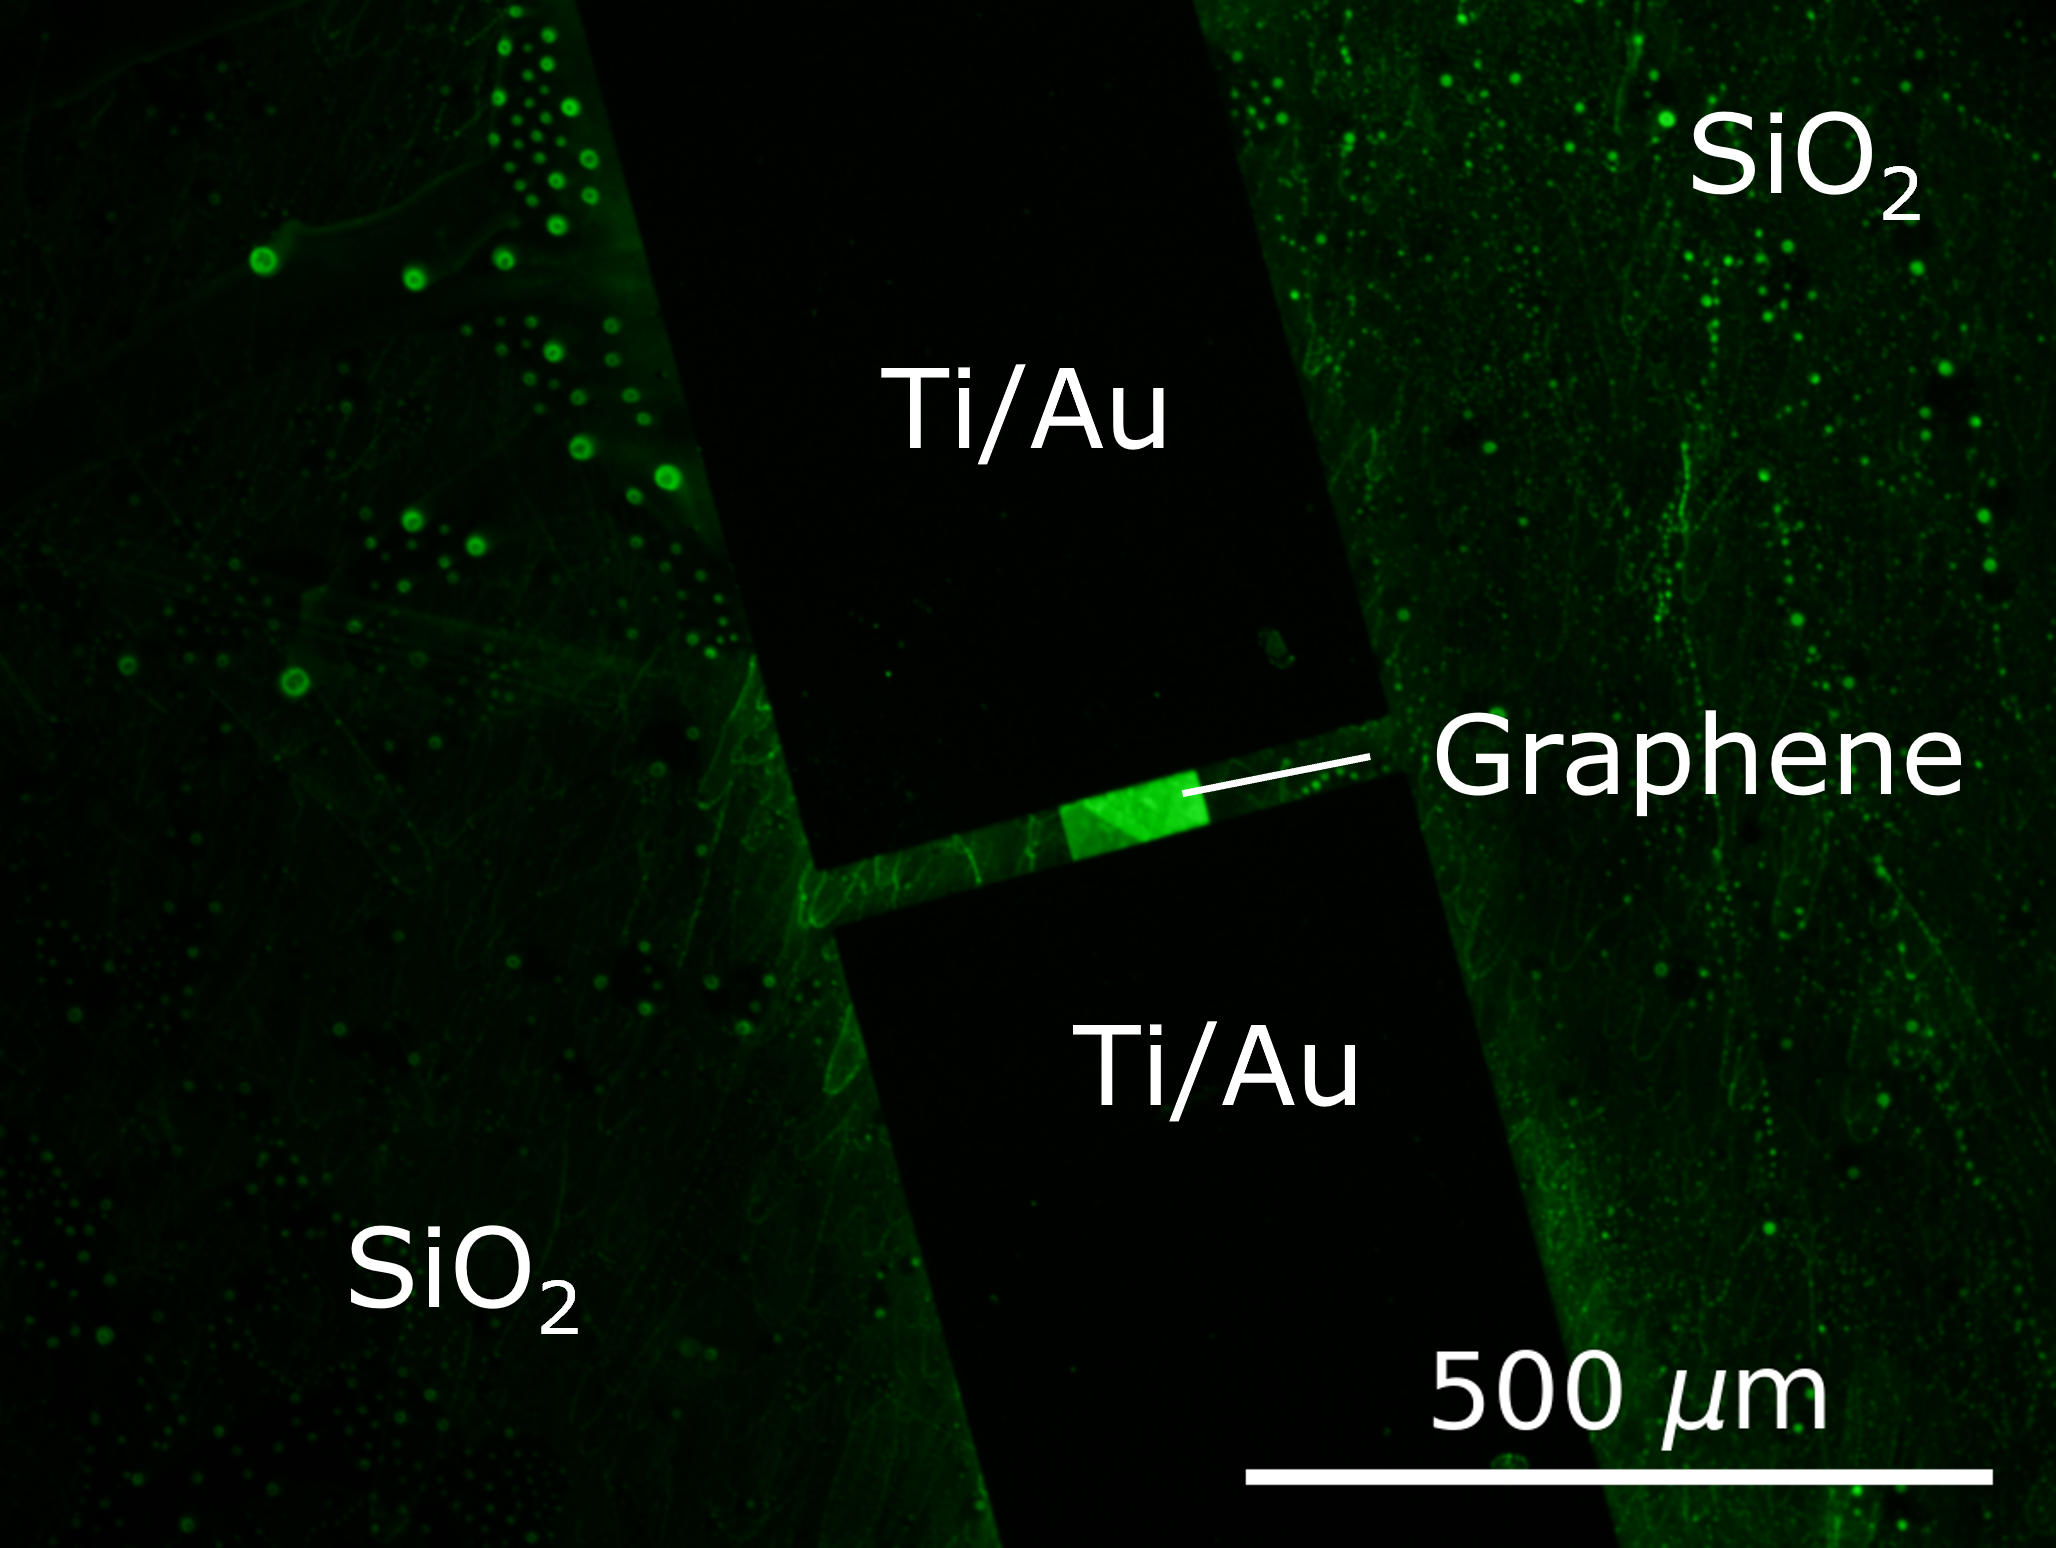
\includegraphics{figures/ch6/labelled_modified_noencap_1mMPPF_channel7_1sexposure_6.3X_highcontrast_221214.png}

}

}

\subcaption{\label{fig-FITC-EtOH-ch7}}
\end{minipage}%

\caption{\label{fig-FITC-EtOH}Fluorescence images of an unencapsulated
graphene channel after functionalisation with 1 mM pyrene-PEG-FITC in
ethanol, taken using an FITC filter with a 1 s exposure time, where (a)
shows channel 2 of the device and (b) shows channel 7. The darker
regions are the device electrodes, while the brightly fluorescent region
is the graphene channel area.}

\end{figure}

\hypertarget{sec-impediments}{%
\section{Addressing Functionalisation Issues}\label{sec-impediments}}

\hypertarget{sec-photoresist-contamination}{%
\subsection{Photoresist
Contamination}\label{sec-photoresist-contamination}}

\begin{figure}

\begin{minipage}[t]{0.47\linewidth}

{\centering 

\raisebox{-\height}{

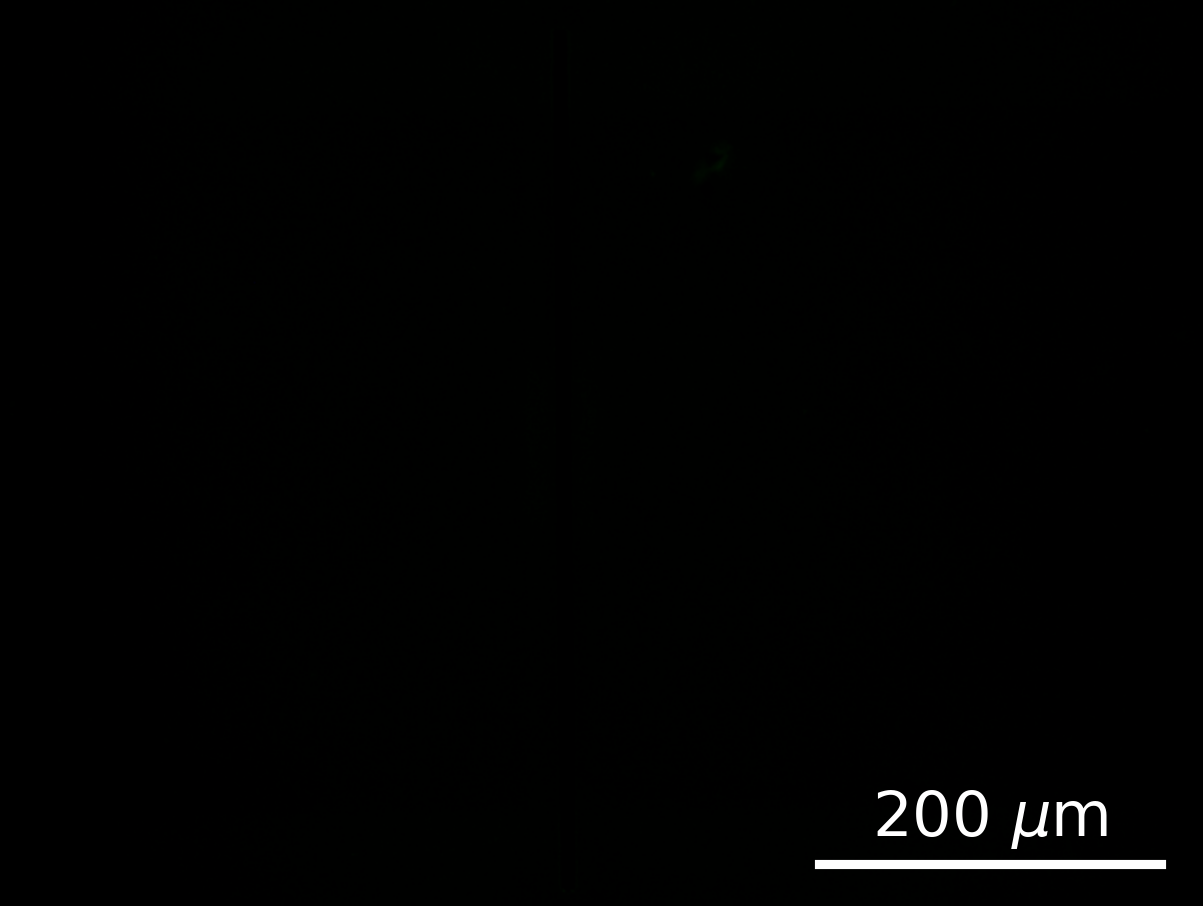
\includegraphics{figures/ch6/modified_SU8only_FITCfilter_channel2_350ms_12.6X_221207.png}

}

}

\subcaption{\label{fig-350ms-SU8}}
\end{minipage}%
%
\begin{minipage}[t]{0.05\linewidth}

{\centering 

~

}

\end{minipage}%
%
\begin{minipage}[t]{0.47\linewidth}

{\centering 

\raisebox{-\height}{

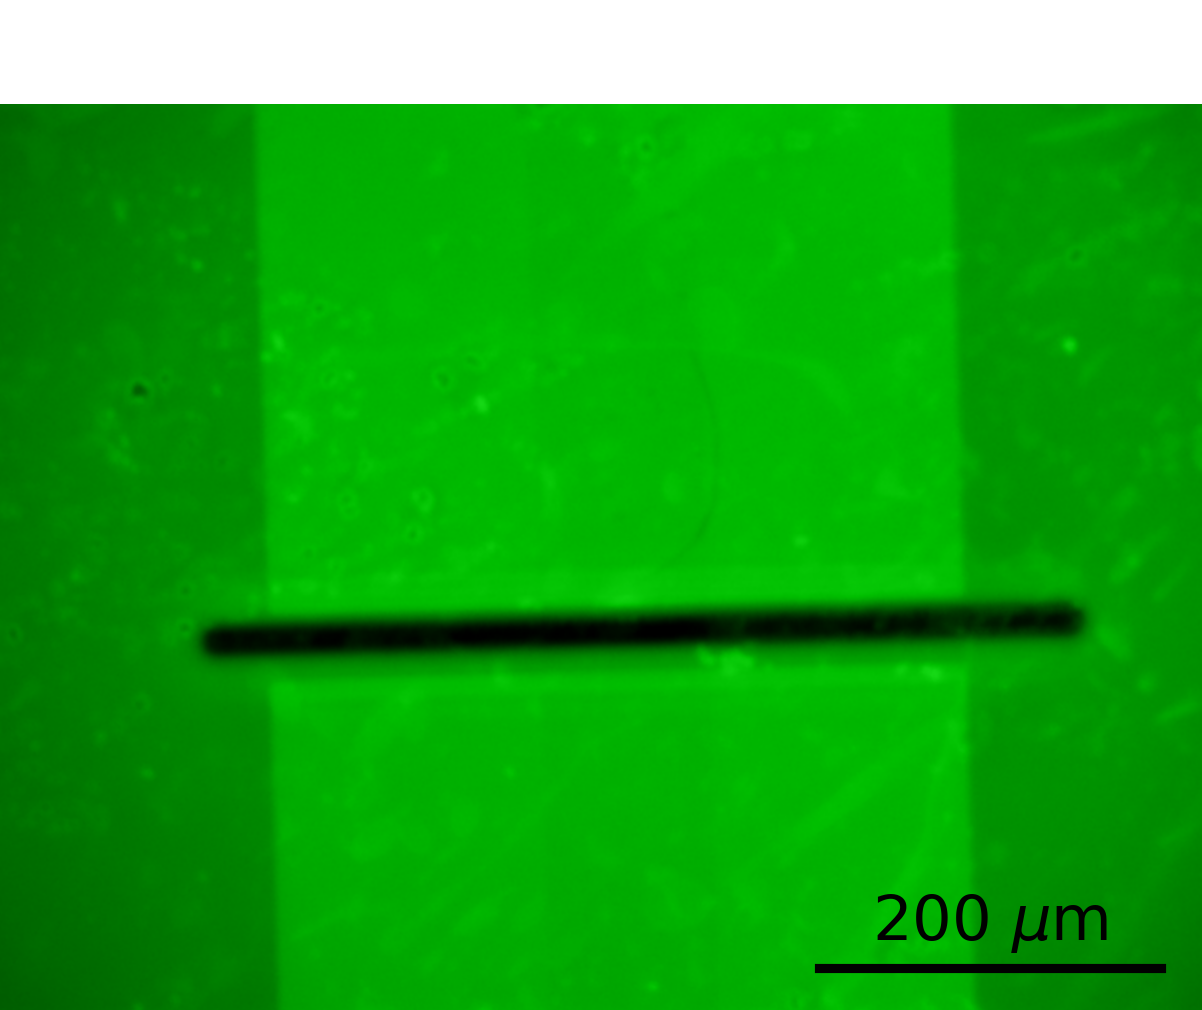
\includegraphics{figures/ch6/modified_CNT20_1mMPPF_channel8_350ms_12.6X_221124.png}

}

}

\subcaption{\label{fig-350ms-SU8-FITC}}
\end{minipage}%
\newline
\begin{minipage}[t]{0.47\linewidth}

{\centering 

\raisebox{-\height}{

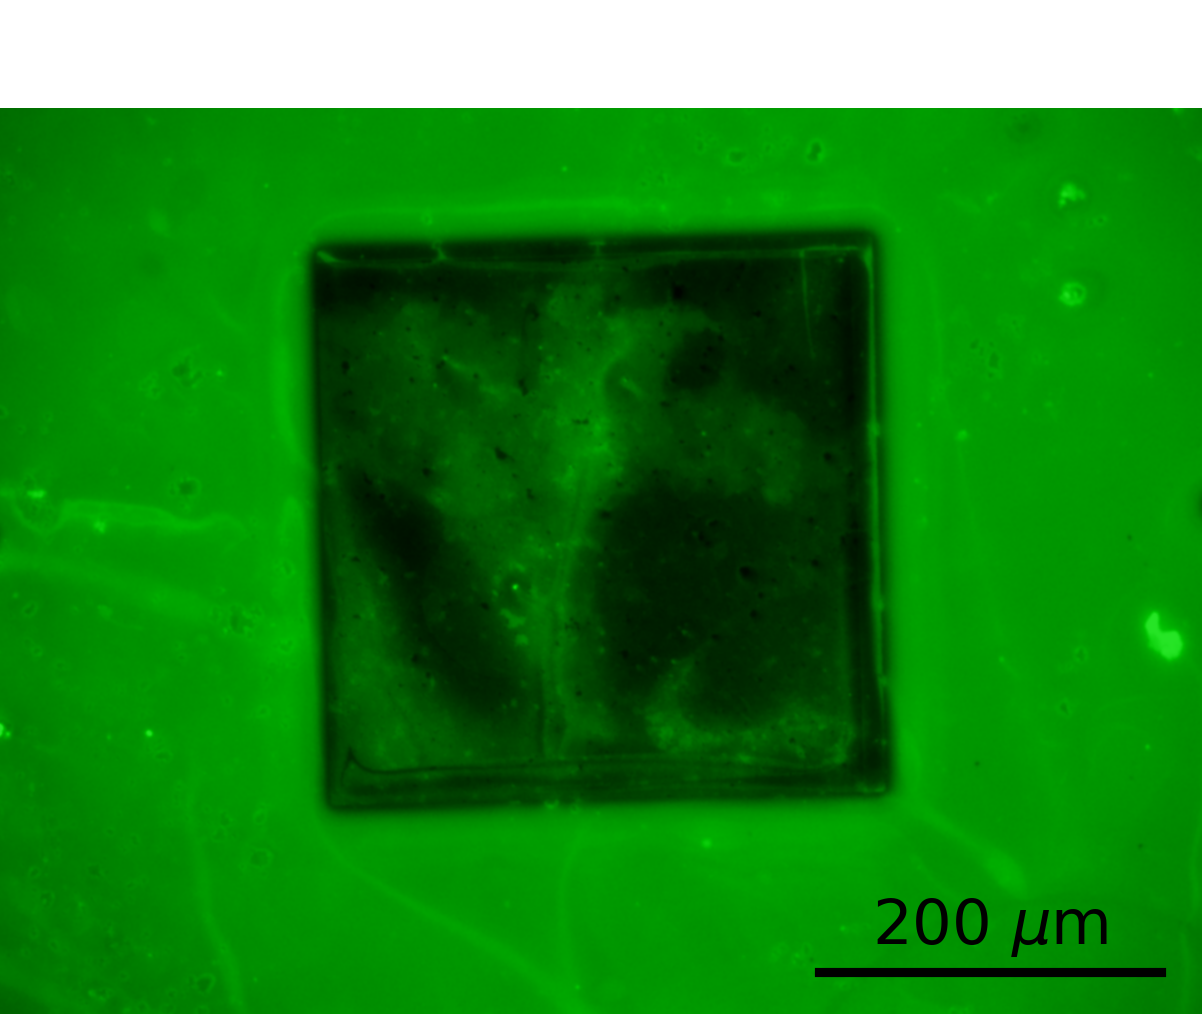
\includegraphics{figures/ch6/modified_CNT20_1mMPPF_window4_350ms_12.6X_221124.png}

}

}

\subcaption{\label{fig-SU8-FITC-CNT}}
\end{minipage}%
%
\begin{minipage}[t]{0.05\linewidth}

{\centering 

~

}

\end{minipage}%
%
\begin{minipage}[t]{0.47\linewidth}

{\centering 

\raisebox{-\height}{

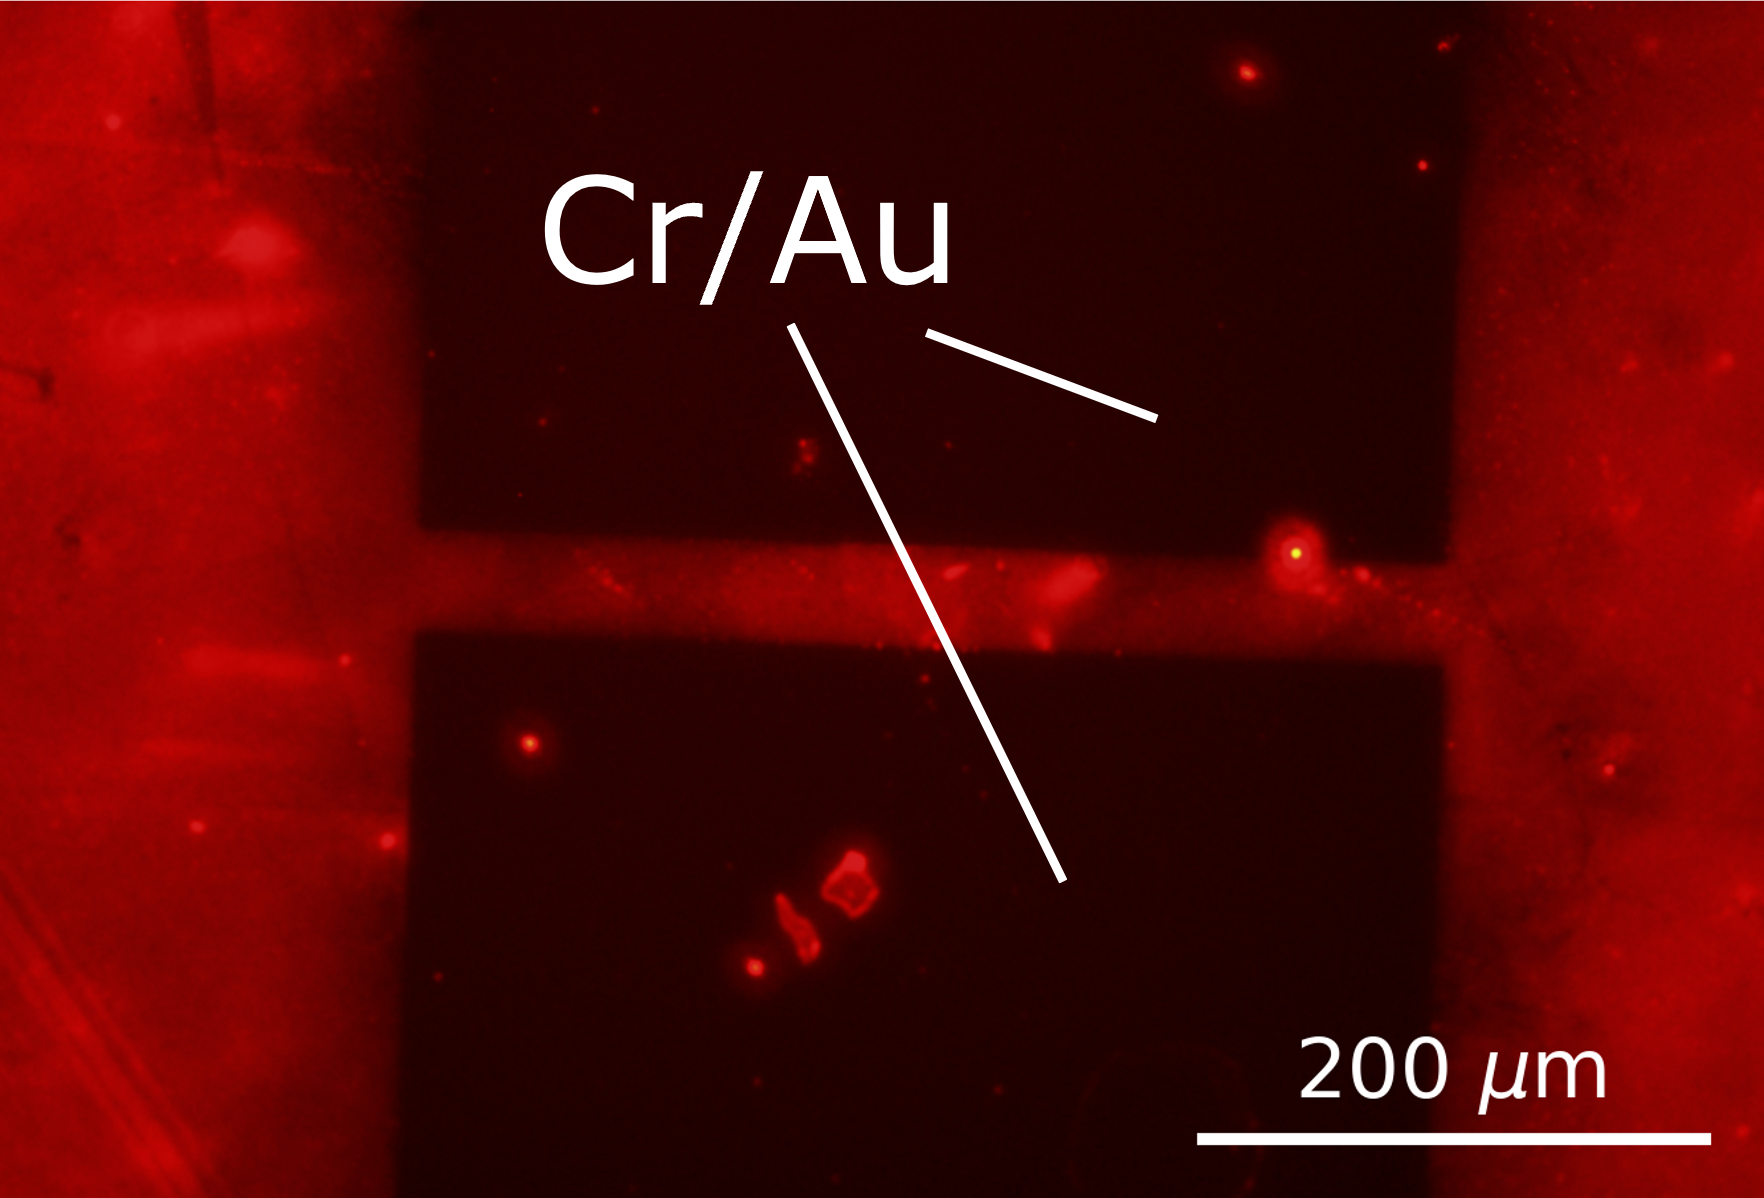
\includegraphics{figures/ch6/modified_softbake1minacetonerinse_aptamer_ch3_mCherry_30sexposure_highcontrast_ISO200_12.6X.png}

}

}

\subcaption{\label{fig-aptamer-photoresist-1}}
\end{minipage}%
\newline
\begin{minipage}[t]{0.26\linewidth}

{\centering 

~

}

\end{minipage}%
%
\begin{minipage}[t]{0.47\linewidth}

{\centering 

\raisebox{-\height}{

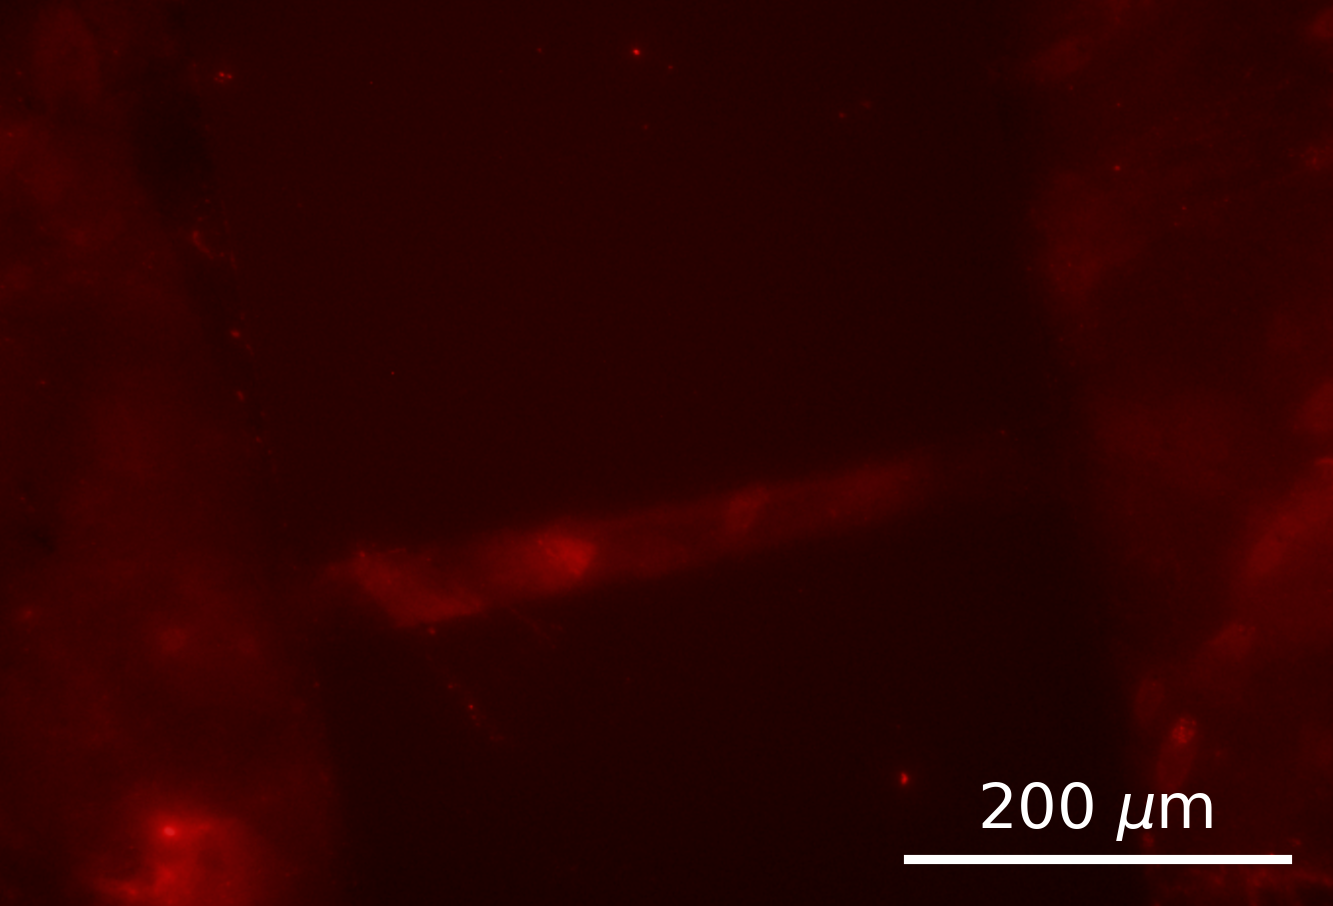
\includegraphics{figures/ch6/modified_hardbake_aptamer_ch3_mCherry_30sexposure_highcontrast_ISO200_12.6X.png}

}

}

\subcaption{\label{fig-aptamer-photoresist-2}}
\end{minipage}%
%
\begin{minipage}[t]{0.26\linewidth}

{\centering 

~

}

\end{minipage}%

\caption{\label{fig-FITC-SU8}A fluorescence image of a carbon nanotube
device encapsulated with SU8 using the pre-2023 mask is shown in (a)
using a 0.35 s exposure time. With the same exposure time as in (a), (c)
shows a SU8-encapsulated channel after modification with an aqueous
solution of 1 mM Pyrene-PEG-FITC, while (d) shows an SU8-coated CNT film
where a 320 \(\mu\)m \(\times\) 320 \(\mu\)m region of SU8 has been
photolithographically removed to expose the CNTs in that region. Both
(d) and (e) show fluorescence images of an carbon nanotube device with
photoresist surface residue after exposure to PBASE and
fluorescent-tagged aptamer, where the device in (e) was hardbaked at
200\(^\circ\)C for 1 hour before exposure while the device (d) was not.
For images (a)-(c) a FITC filter was used, while for (d)-(e) a mCherry
filter and 30 s exposure time were used.}

\end{figure}

An functionalisation issue quickly encountered when characterising
pyrene-PEG-FITC interaction with device channels (PPF) via fluorescence
microscopy was an unwanted secondary interaction between the linker and
residual photoresist. Figure~\ref{fig-350ms-SU8} and
Figure~\ref{fig-350ms-SU8-FITC} are fluorescence images of SU8
encapsulation before and after being exposed to PPF. Despite the same
microscope settings being used to take the images (filter, ISO,
contrast, exposure time), the SU8 exposed to PPF appears much brighter
than the pristine SU8. No fluorescence is seen from the device channel,
as the length of exposure time required to see the fluorescence would
lead to fluorescence from the dye-modified linker attached to the
photoresist flooding the image with light. An analogy which could be
used is that of a dim outdoor lamp in a photograph; if the photograph
was taken on a starless night, it would show up clearly, but with the
sun out it would be very difficult to see regardless of how the
photograph was taken. We therefore assert that because the fluorescence
of the dye attached to the photoresist is much more intense than the dye
attached to the carbon nanotubes, the linker appears to have a more
extensive interaction with the photoresist via an unknown mechanism than
it does by \(pi\)-stacking with the carbon nanotubes.

Figure~\ref{fig-SU8-FITC-CNT} shows a square region of carbon nanotubes
surrounded by photoresist after exposure to PFF. Some patches of the
carbon nanotube square appear brighter than others. Since we know that
dye-modified linker attached to photoresist has a greater fluorescent
intensity than dye-modified linker attached to carbon nanotubes, it
appears that these bright patches correspond to patches of residual
photoresist which have not been completely removed from the carbon
nanotube square by the development process. A similar interaction
between AZ\(^\circledR\) 1518 photoresist and fluorescent-tagged,
amine-terminated aptamer was seen when functionalising using PBASE, as
seen in \textbf{?@fig-aptamer-photoresist}. The presence of photoresist
residue is undesirable for both functionalisation and sensing, and
fluorescence microscopy was a useful tool for detecting residue and
testing suitable residue elimination measures.

Two carbon nanotube network devices were spincoated with
AZ\(^\circledR\) 1518 photoresist and heated at 95\(^\circ\)C for 5
minutes. One device was then hardbaked at 200\(^\circ\)C for 1 hour.
Both devices were then rinsed for 1 minute with acetone. Each device was
then submerged in 1 mM PBASE in methanol for 1 hour, rinsed with
methanol and Tris buffer, then incubated in 1 \(\mu\)M Cy3-tagged
aptamer in Tris buffer at 4\(^\circ\)C overnight. The aptamer was
denatured by heating in a water bath at 95\(^\circ\)C for 5 minutes then
cooling in an ice bath for 10 minutes before use. Fluorescence
microscope images of channels from the two devices are shown in
\textbf{?@fig-aptamer-photoresist}, where the dark regions are the gold
device electrodes.

From comparing Figure~\ref{fig-aptamer-photoresist-1} and
Figure~\ref{fig-aptamer-photoresist-2}, it is apparent that hardbaking
the AZ\(^\circledR\) 1518 photoresist significantly reduces the amount
of fluorescent aptamer attached to the surface. This is an indication
that the chemical interaction between the photoresist and the pyrene
linker, or alternatively the biological material, can be suppressed
through sufficient heating of the photoresist. Hardbaking of the
photoresist does not appear to have completely prevented
functionalisation, with some aptamer fluorescence still visible in
Figure~\ref{fig-aptamer-photoresist-2}. It is possible that heating from
the bottom of the device is insufficient to hardbake the photoresist
layer completely, an effect that would be amplified for the thick
photoresist layer on encapsulated devices. Therefore, from June 2023
onwards devices were vacuum annealed for 1 hour at 150 \(^\circ\)C prior
to functionalisation. This approach was taken to ensure photoresist was
being heated from above as well as below and made chemically inert at
its surface.

Using fluorescence microscopy, an effective measure for remove exposed
to UV light and placed in AZ\(^\circledR\) 326 developer to remove
residual photoresist after each photolithography step.

\hypertarget{sec-hydrophobicity}{%
\subsection{Hydrophobicity of Carbon Nanotubes and
Graphene}\label{sec-hydrophobicity}}

\begin{figure}

\begin{minipage}[t]{0.47\linewidth}

{\centering 

\raisebox{-\height}{

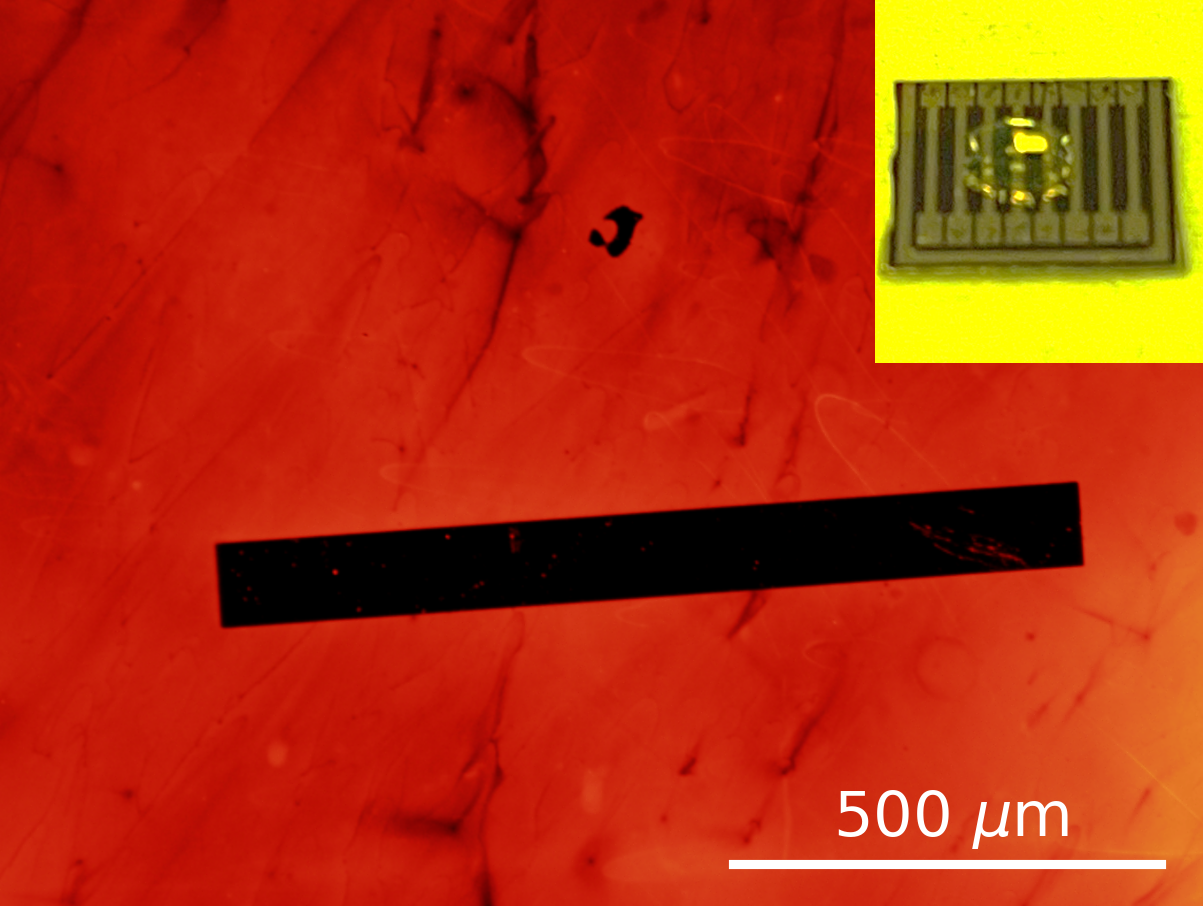
\includegraphics{figures/ch6/modified_NGW8D9_edgechannel_post10min50Cacetonerinse_221109.png}

}

}

\subcaption{\label{fig-no-attachment}}
\end{minipage}%
%
\begin{minipage}[t]{0.05\linewidth}

{\centering 

~

}

\end{minipage}%
%
\begin{minipage}[t]{0.47\linewidth}

{\centering 

\raisebox{-\height}{

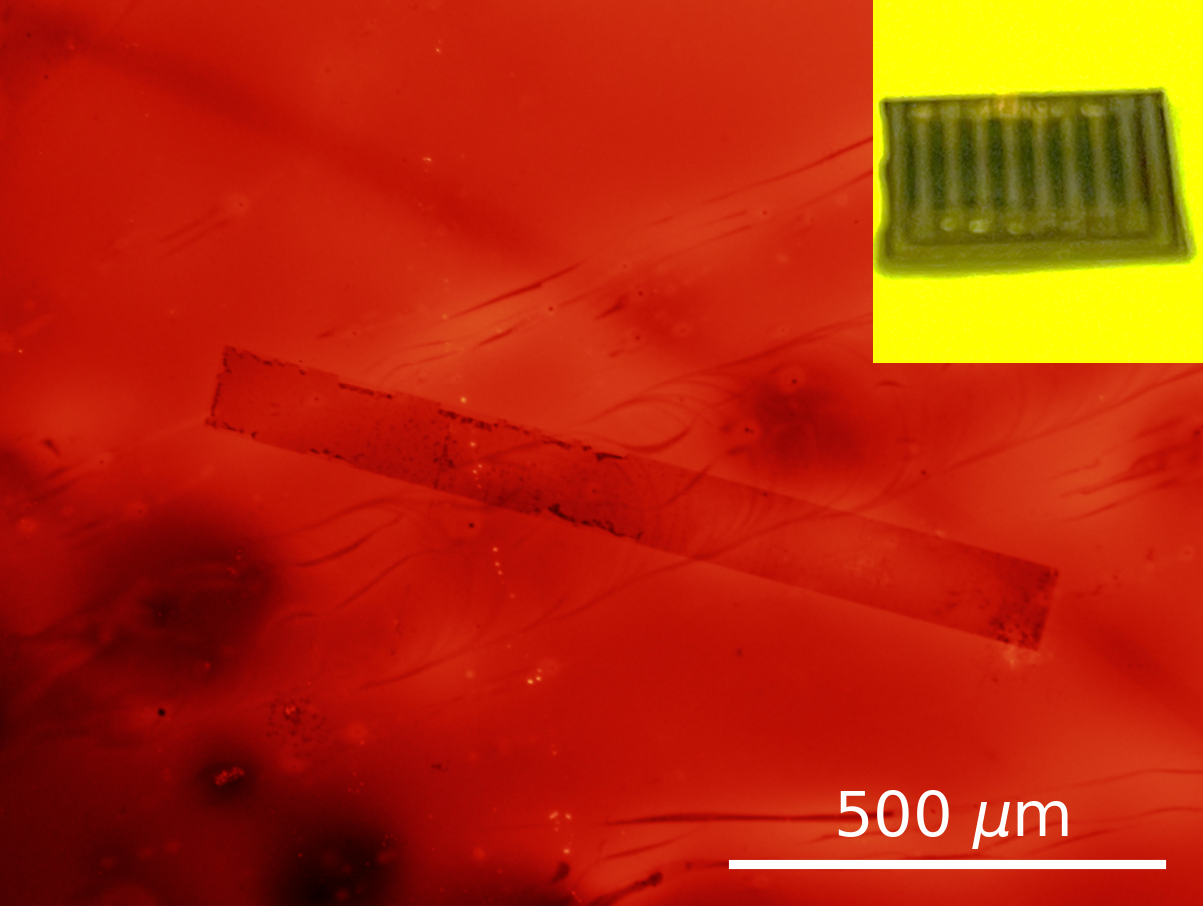
\includegraphics{figures/ch6/modified_NGW8D7_edgechannel_lowerexposuretime_221108.png}

}

}

\subcaption{\label{fig-attachment-post-plasma}}
\end{minipage}%

\caption{\label{fig-hydrophobicity}Fluorescence images of a 1000
\(\mu\)m \(\times\) 100 \(\mu\)m graphene channel after
functionalisation with 1 mM pyrene-PEG-rhodamine in 1XPBS, taken using
an Texas Red filter and a 1.8 s exposure time. The graphene film in (a)
was not oxygen plasma cleaned before functionalisation, while the
graphene film in (b) was oxygen plasma cleaned at 5 W for 15 s at 300
mTorr pressure immediately before functionalisation. Insets show a 10
\(\mu\)L droplet placed on an unencapsulated carbon nanotube device
before (a) and after (b) the same oxygen plasma treatment procedure.}

\end{figure}

As PEGlyated linker dissolves well in aqueous solution, initial
fluorescence imaging focused on functionalising devices with these
linkers dissolved in 1XPBS. It was hoped that by keeping the device
channels in a pH-controlled environment, the channel surface would be
made more suitable for the attached receptors.
Figure~\ref{fig-no-attachment} shows a graphene film after exposure to
pyrene-PEG-rhodamine (PPR) in 1XPBS solution for 1 hour. The
pyrene-PEG-rhodamine has interacted with the silicon dioxide substrate
(discussed further in Section~\ref{sec-pyrene-interactions}) but not the
graphene film. The graphene does not attach to the pyrene or rhodamine
due to the highly hydrophobic graphene surface repelling the surrounding
solution, preventing \(\pi\)-stacking from occurring. The hydrophobicity
of the graphene surface is not intrinsic to graphene (or to carbon
nanotubes), and instead results from a hydrocarbonaceous layer which
forms on the graphene (or carbon nanotube) surface when exposed to air
\autocite{Ashraf2014,Stando2019,Park2022}. Treatment with oxygen plasma
at 5 W for 15 s has previously been found to remove this
hydrocarbonaceous layer, restoring the intrinsic hydrophilicity of
graphene \autocite{Shin2010}. Storing the graphene surface in DI water
rather than air prevents the return of this hydrocarbon layer
\autocite{Ashraf2014}. The use of a relatively low power plasma ensures
damage to the graphene layer is minimised.

Treatment of an unencapsulated carbon nanotube network device at 5 W for
15 s at 300 mTorr greatly reduced the contact angle of a water droplet
placed on the device surface, shown inset in
Figure~\ref{fig-hydrophobicity} before and after plasma treatment. A
graphene film was then functionalised with pyrene-PEG-rhodamine in 1XPBS
in the same manner as for the film in Figure~\ref{fig-no-attachment},
except with the same plasma treatment performed on the film less than 1
minute before functionalisation. The result is shown in
Figure~\ref{fig-attachment-post-plasma}. The graphene now appears to
interact with the pyrene-PEG-rhodamine. These results both indicate that
the plasma treatment is increasing the hydrophilicity of the device
surface, improving the ability of pyrene-PEG-rhodamine to \(\pi\)-stack
with graphene. The disadvantage of this procedure is that the plasma
cleaning introduces defects to the graphene surface which may be
undesirable for device electrical behaviour. Furthermore, it was often
found that devices functionalised in this manner had their conductance
drop significantly after functionalisation, even though plasma treatment
itself did not significantly alter device conductance. Solvent was
therefore used for the initial linker functionalisation in
Section~\ref{sec-linker-receptor-attachment}, as it did not require a
plasma cleaning step for successful attachment.

\begin{figure}

\begin{minipage}[t]{0.47\linewidth}

{\centering 

\raisebox{-\height}{

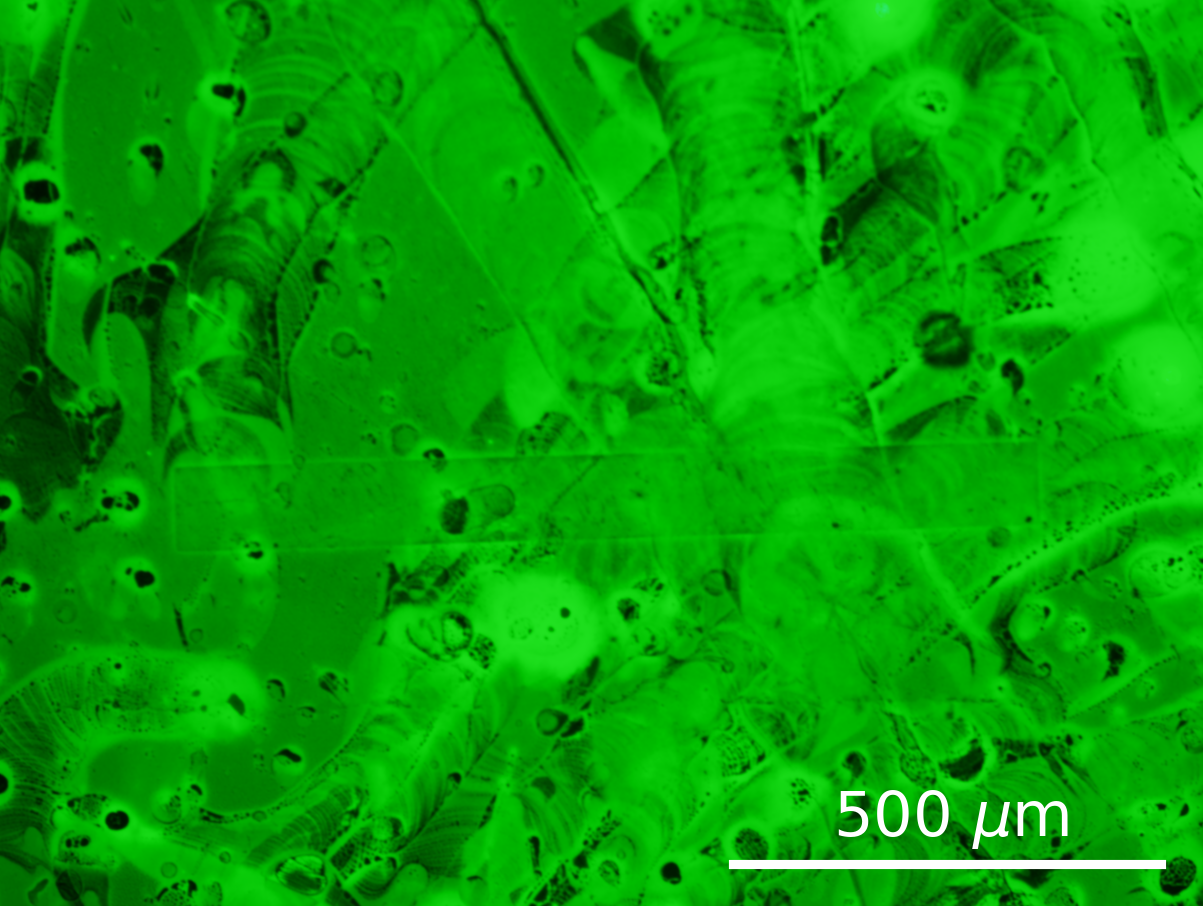
\includegraphics{figures/ch6/modified_NGW6D4_PyPEGFITC_channel2_1.6sexposure_10X_221122.png}

}

}

\subcaption{\label{fig-FITC-silicon-dioxide}}
\end{minipage}%
%
\begin{minipage}[t]{0.05\linewidth}

{\centering 

~

}

\end{minipage}%
%
\begin{minipage}[t]{0.47\linewidth}

{\centering 

\raisebox{-\height}{

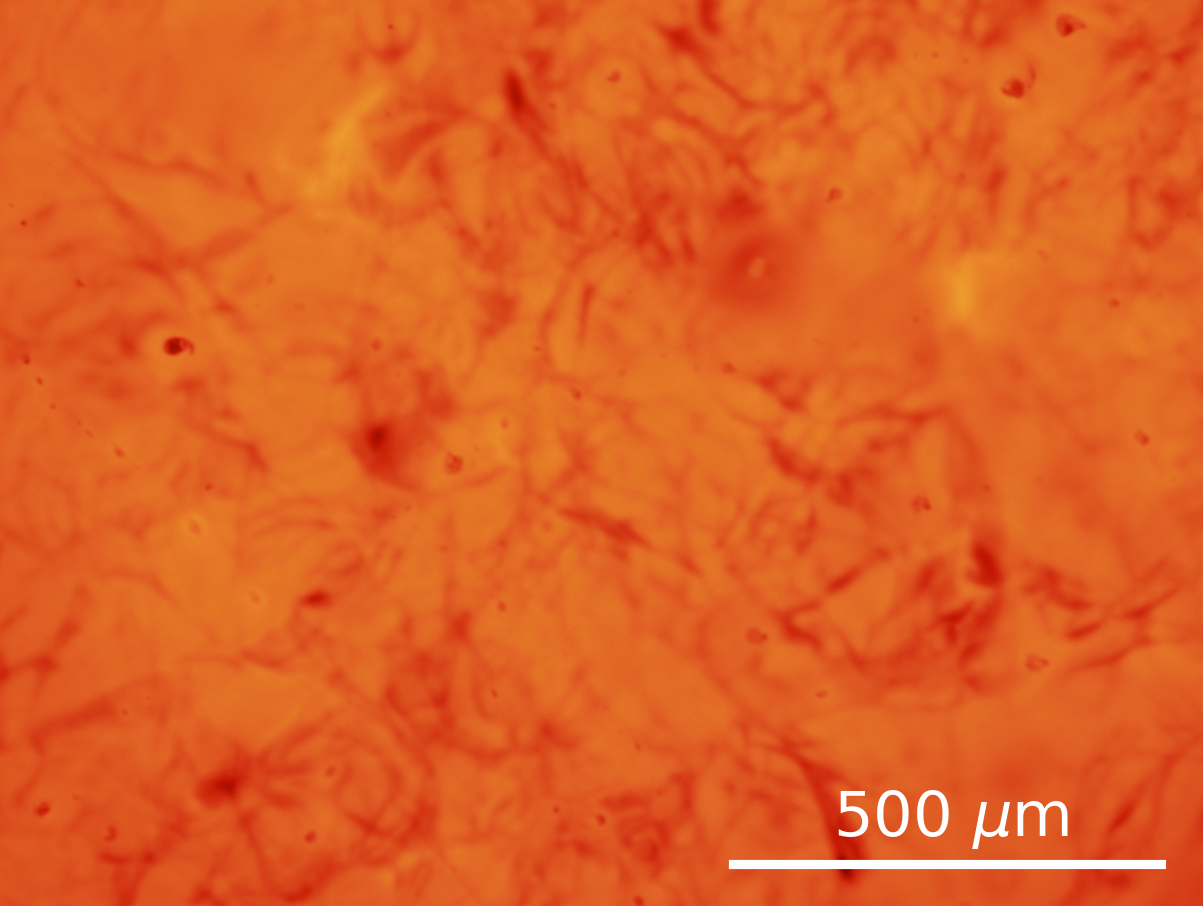
\includegraphics{figures/ch6/modified_SiO2_1mMPPR_2_221109.png}

}

}

\subcaption{\label{fig-rhodamine-silicon-dioxide}}
\end{minipage}%
\newline
\begin{minipage}[t]{0.47\linewidth}

{\centering 

\raisebox{-\height}{

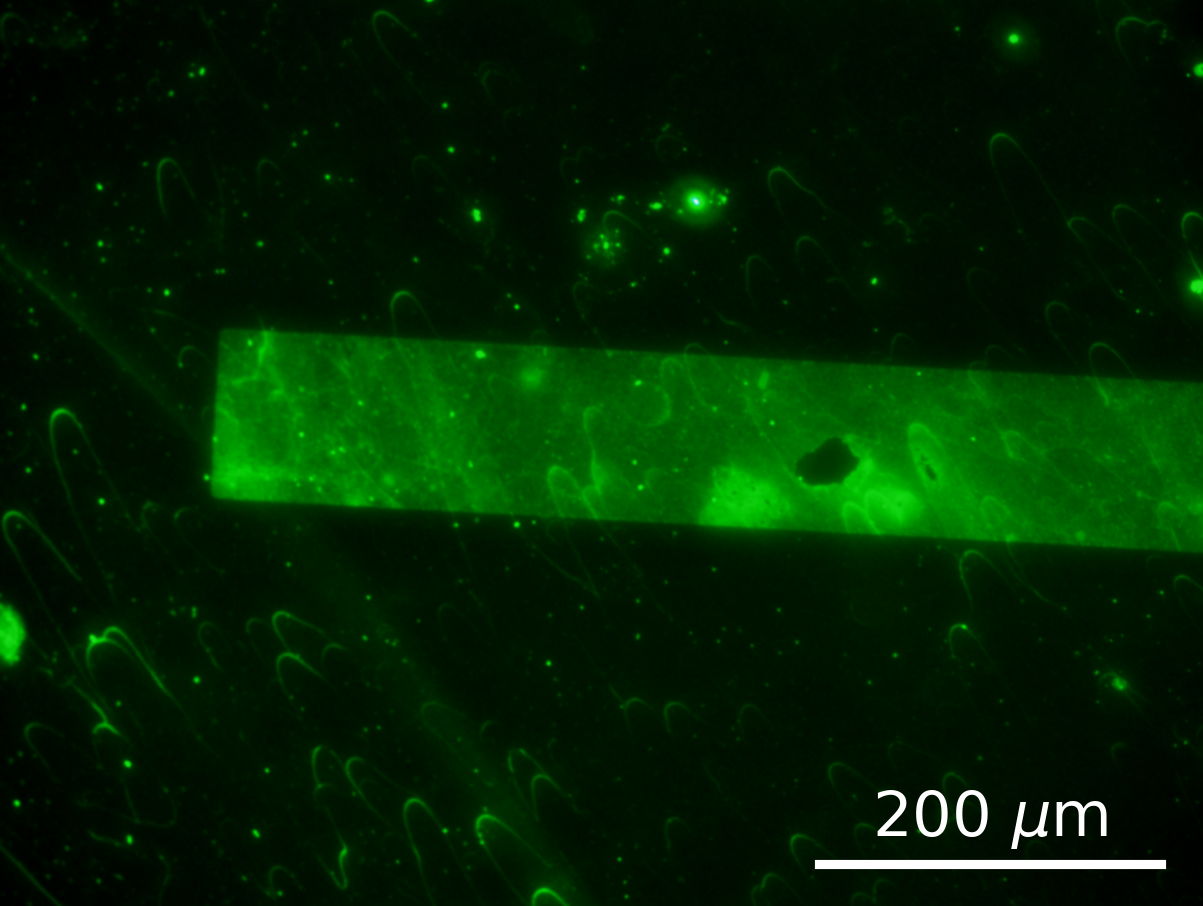
\includegraphics{figures/ch6/modified_NGW6D7_PyPEGFITC_channel3top_postmsurfclean_7.5sexposure_20X_221123.png}

}

}

\subcaption{\label{fig-PPF-PBS-20X}}
\end{minipage}%
%
\begin{minipage}[t]{0.05\linewidth}

{\centering 

~

}

\end{minipage}%
%
\begin{minipage}[t]{0.47\linewidth}

{\centering 

\raisebox{-\height}{

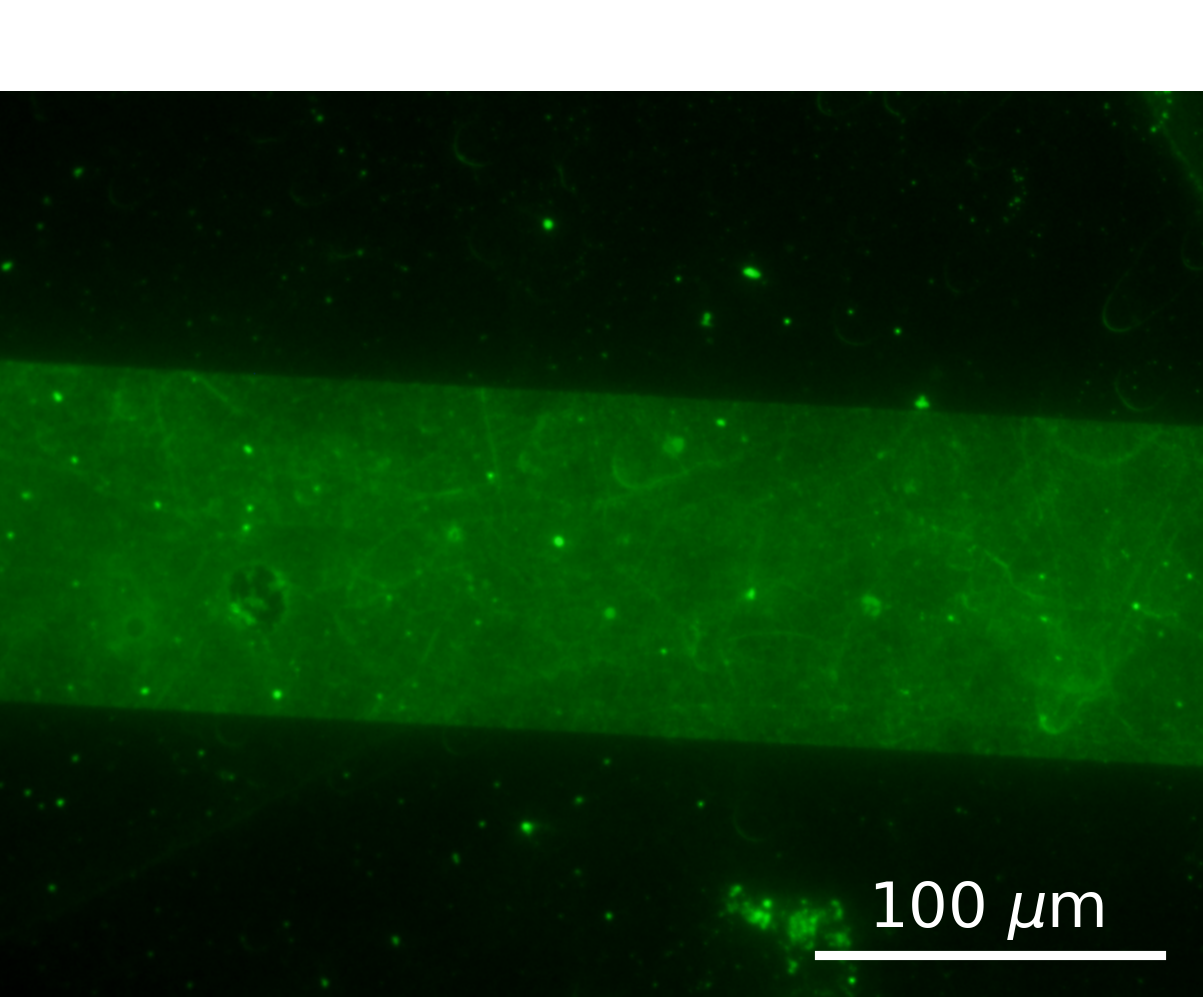
\includegraphics{figures/ch6/modified_NGW6D7_PyPEGFITC_channel1_postmsurfclean_7.75sexposure_40X_221123.png}

}

}

\subcaption{\label{fig-PPF-PBS-40X}}
\end{minipage}%

\caption{\label{fig-silicon-dioxide-interaction}The 1000 \(\mu\)m
\(\times\) 100 \(\mu\)m graphene film in image (a) was functionalised
with 1 mM pyrene-PEG-FITC in 1XPBS after oxygen plasma treatment, taken
using an FITC filter and a 1.6 s exposure time. (b) shows a silicon
dioxide surface which had never been exposed to carbon nanotubes,
graphene or photoresist after exposure to 1 mM pyrene-PEG-rhodamine in
1XPBS, taken using a Texas Red filter and a 1.8 s exposure time.
Graphene films on a substrate functionalised with 1 mM pyrene-PEG-FITC
in 1XPBS after oxygen plasma treatment then cleaned with m-CNT
dispersion surfactant (NanoIntegris) are shown in (c) and (d), where a
FITC filter was used, with 7.5 s and 7.75 s exposure times
respectively.}

\end{figure}

\hypertarget{sec-pyrene-interactions}{%
\subsection{Substrate Interaction with Linker
Molecules}\label{sec-pyrene-interactions}}

Another issue that arose when verifying surface functionalisation was
the interaction between pyrene linker and the silicon dioxide substrate.
This interaction meant it was difficult to discern whether the pyrene
group was interacting in a specific manner with the channel film. It was
confirmed that pyrene-PEG was interacting with silicon dioxide, rather
than residual photoresist or nanomaterial, by performing a
pyrene-PEG-rhodamine functionalisation on pristine silicon dioxide, as
shown in Figure~\ref{fig-rhodamine-silicon-dioxide}. The PEGlyated
linker supplier suggested that the surface should be thoroughly rinsed
with surfactant to remove weakly-bound pyrene-PEG-FITC attached to the
silicon dioxide, while preserving the pyrene-PEG-FITC strongly attached
via \(\pi\)-stacking to the graphene or carbon nanotube film
\autocite{CreativePEGworks2022}. The following process was then used to
remove pyrene-PEG-FITC from the silicon dioxide: the film was rinsed
with DI water for 30 s, then placed in m-CNT dispersion solution
(NanoIntegris) for 5 minutes at 70\(^\circ\)C while agitating with a
pipette, and finally rinsed with DI water, ethanol, acetone, IPA and
nitrogen dried. The results of this thorough cleaning process are shown
in Figure~\ref{fig-PPF-PBS-20X} and Figure~\ref{fig-PPF-PBS-40X}. The
majority of pyrene-PEG-FITC was removed in regions with no graphene, but
remained where graphene was present, indicating specific,
\(\pi\)-stacking interaction took place between the pyrene-PEG-FITC and
graphene.

\hypertarget{sec-coffee-ring}{%
\subsection{``Coffee-Ring'' Effect}\label{sec-coffee-ring}}

\begin{figure}

\begin{minipage}[t]{0.47\linewidth}

{\centering 

\raisebox{-\height}{

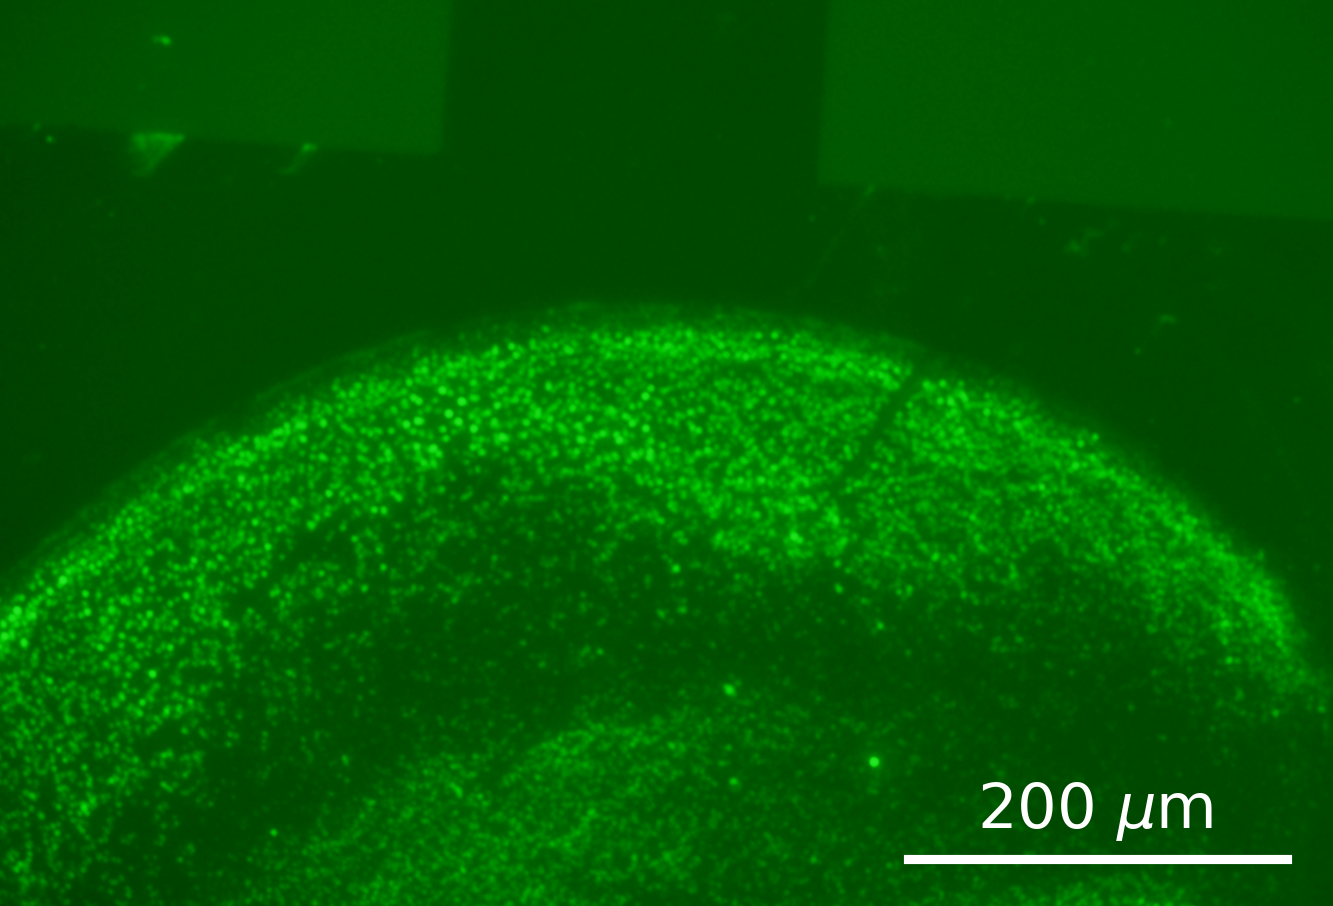
\includegraphics{figures/ch6/modified_GFPNi2+1_5sexposure_12.6X_mediumcontrast_18_230324.png}

}

}

\subcaption{\label{fig-GFP-coffee-ring-1}}
\end{minipage}%
%
\begin{minipage}[t]{0.05\linewidth}

{\centering 

~

}

\end{minipage}%
%
\begin{minipage}[t]{0.47\linewidth}

{\centering 

\raisebox{-\height}{

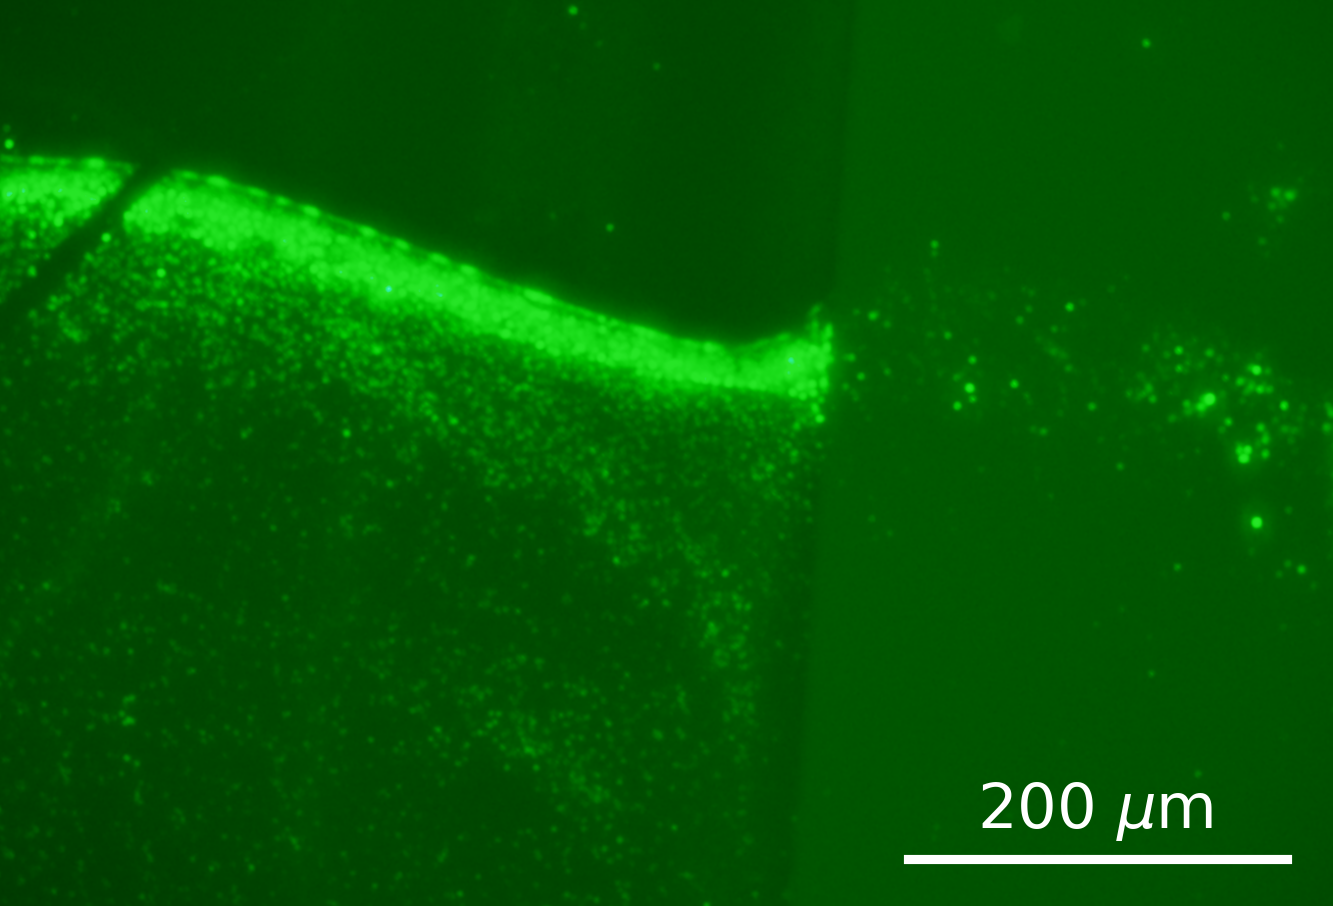
\includegraphics{figures/ch6/modified_GFPNi2+1_5sexposure_12.6X_mediumcontrast_20_230324.png}

}

}

\subcaption{\label{fig-GFP-coffee-ring-2}}
\end{minipage}%

\caption{\label{fig-GFP-coffee-ring}Both (a) and (b) show a build-up of
his-tag GFP at the edges of the droplet region where pyrene-PEG-NTA had
been present, taken using an GFP filter and a 5 s exposure time. On the
right hand side of (b), no his-tag GFP is visible on the metal
electrode, as no pyrene-PEG attaches to the metal electrodes.}

\end{figure}

From Table~\ref{tbl-pbase-functionalisation}, full device submersion
appears to be the most common approach for functionalisation with
solution containing linker molecules like PBASE. However, some groups
placed small droplets of solution onto the device channels when
functionalisation, and this approach was tested as part of the
fluorescence verification work. For functionalisation with his-tagged
green fluorescent protein, after plasma cleaning at 5 W for 15 s at 300
mTorr, a 4 \(\mu\)L droplet of 100\(\mu\)M pyrene-PEG-NTA in 1XPBS was
placed on each graphene device channel and left covered in a humid
environment for 15 minutes. The device was then rinsed with 1XPBS,
submerged in 10 mM NiSO\(_4\) in 1XPBS for 1 hour, rinsed in 1XPBS then
submerged in 10 mL of 100 ng/mL his-tag GFP solution (Thermofisher)
overnight. Fluorescence microscope imaging showed that a ring of
biomaterial would build up around the outer edge of regions where
pyrene-PEG-NTA had been present, as seen in
Figure~\ref{fig-GFP-coffee-ring}.

It appears this is a result of the his-tag GFP attaching to a dense
region of pyrene-PEG-NTA at the edge of the functionalisation droplet.
This accretion of pyrene-PEG-NTA at the edge of the droplet is a result
of the coffee-ring effect, where the evaporation of the droplet leads to
transport of particles to the droplet edges via capillary flow
\autocite{Deegan1997,Shimobayashi2018}. As the effecs of having a large
gradient in the surface coverage of attached protein across the device
surface have unknown consequences for sensing, in functionalisation
processes performed after this test the devices were incubated with
PBASE or pyrene-PEG-NTA by submerging them in solution, rather than
using the dropcasting approach.

\hypertarget{sec-linker-receptor-attachment}{%
\section{Verifying Linker-OR Nanodisc
Attachment}\label{sec-linker-receptor-attachment}}

\hypertarget{sec-PBASE-GFP-OR-attachment}{%
\subsection{Functionalisation using
PBASE}\label{sec-PBASE-GFP-OR-attachment}}

To verify the formation of amide (or imide) bonds between PBASE and the
odorant receptors (ORs) contained within nanodiscs, a fluorescent
biomarker was directly attached to the odorant receptors for detection
with fluorescence microscopy. The biomarker used was the \emph{Aequorea
Victoria} green fluorescent protein (GFP). As far as I know, this is the
first time fluorescence has been used to verify the successful
attachment of odorant receptor nanodiscs to a carbon nanotube network.

\begin{figure}

\begin{minipage}[t]{0.47\linewidth}

{\centering 

\raisebox{-\height}{

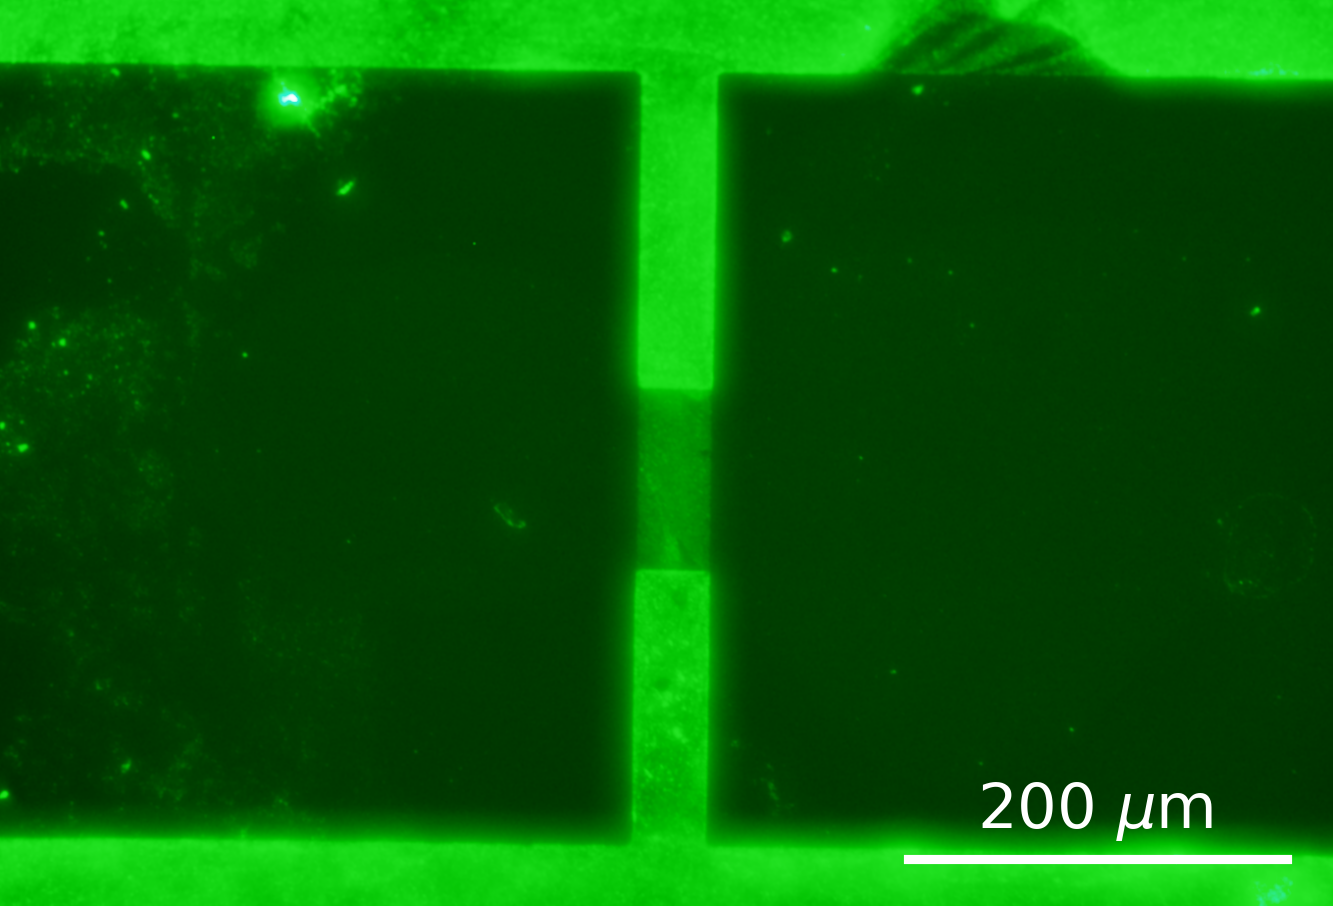
\includegraphics{figures/ch6/modified_GFPOR_PBASE_10sexposure_20X_mediumcontrast_ch1_231019_2.png}

}

}

\subcaption{\label{fig-PBASE-GFP-OR-ch3-zoom}}
\end{minipage}%
%
\begin{minipage}[t]{0.05\linewidth}

{\centering 

~

}

\end{minipage}%
%
\begin{minipage}[t]{0.47\linewidth}

{\centering 

\raisebox{-\height}{

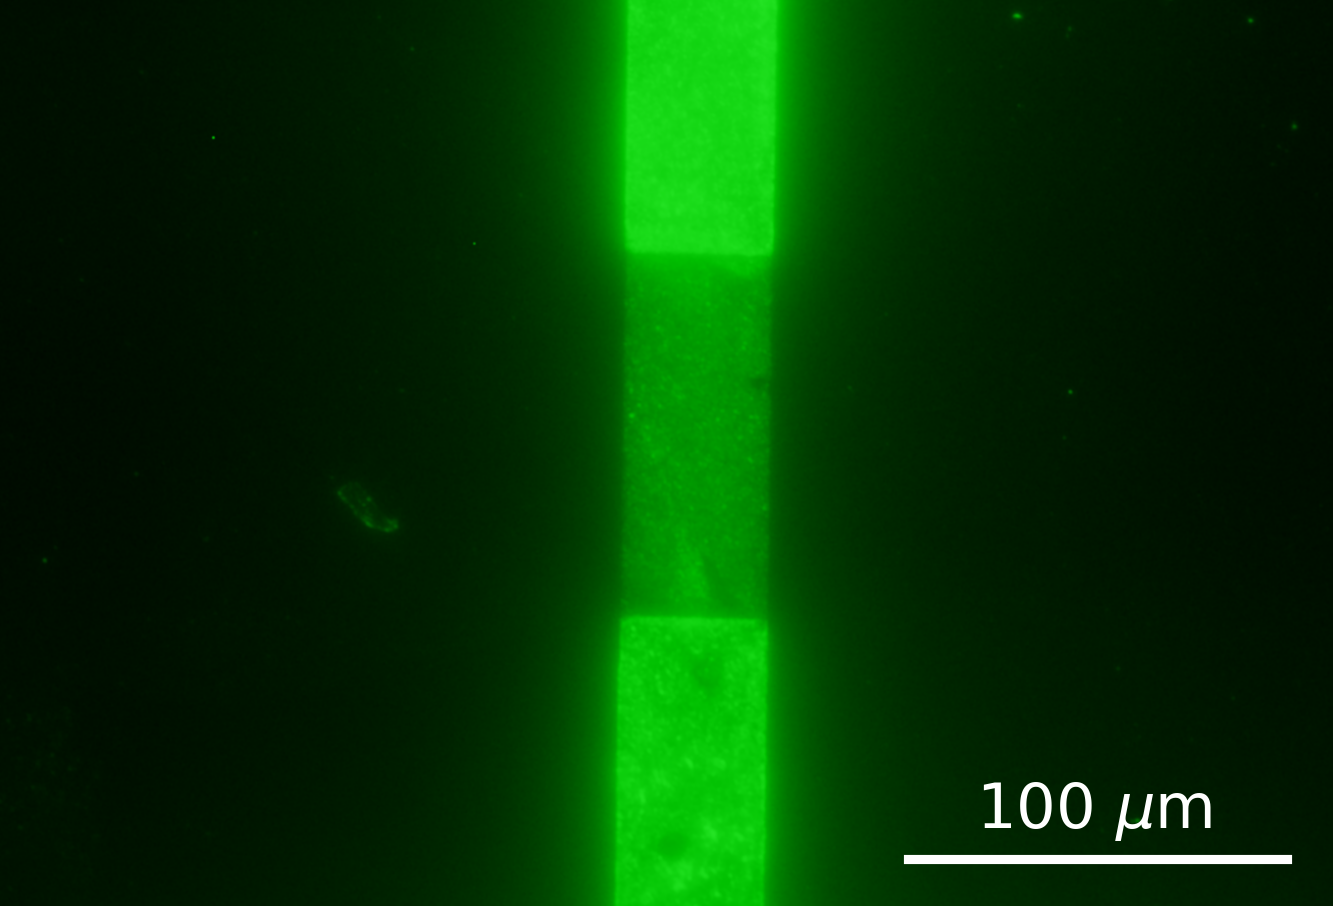
\includegraphics{figures/ch6/modified_GFPOR_PBASE_10sexposure_40X_mediumcontrast_ch1_231019_2.png}

}

}

\subcaption{\label{fig-PBASE-GFP-OR-ch1}}
\end{minipage}%
\newline
\begin{minipage}[t]{0.47\linewidth}

{\centering 

\raisebox{-\height}{

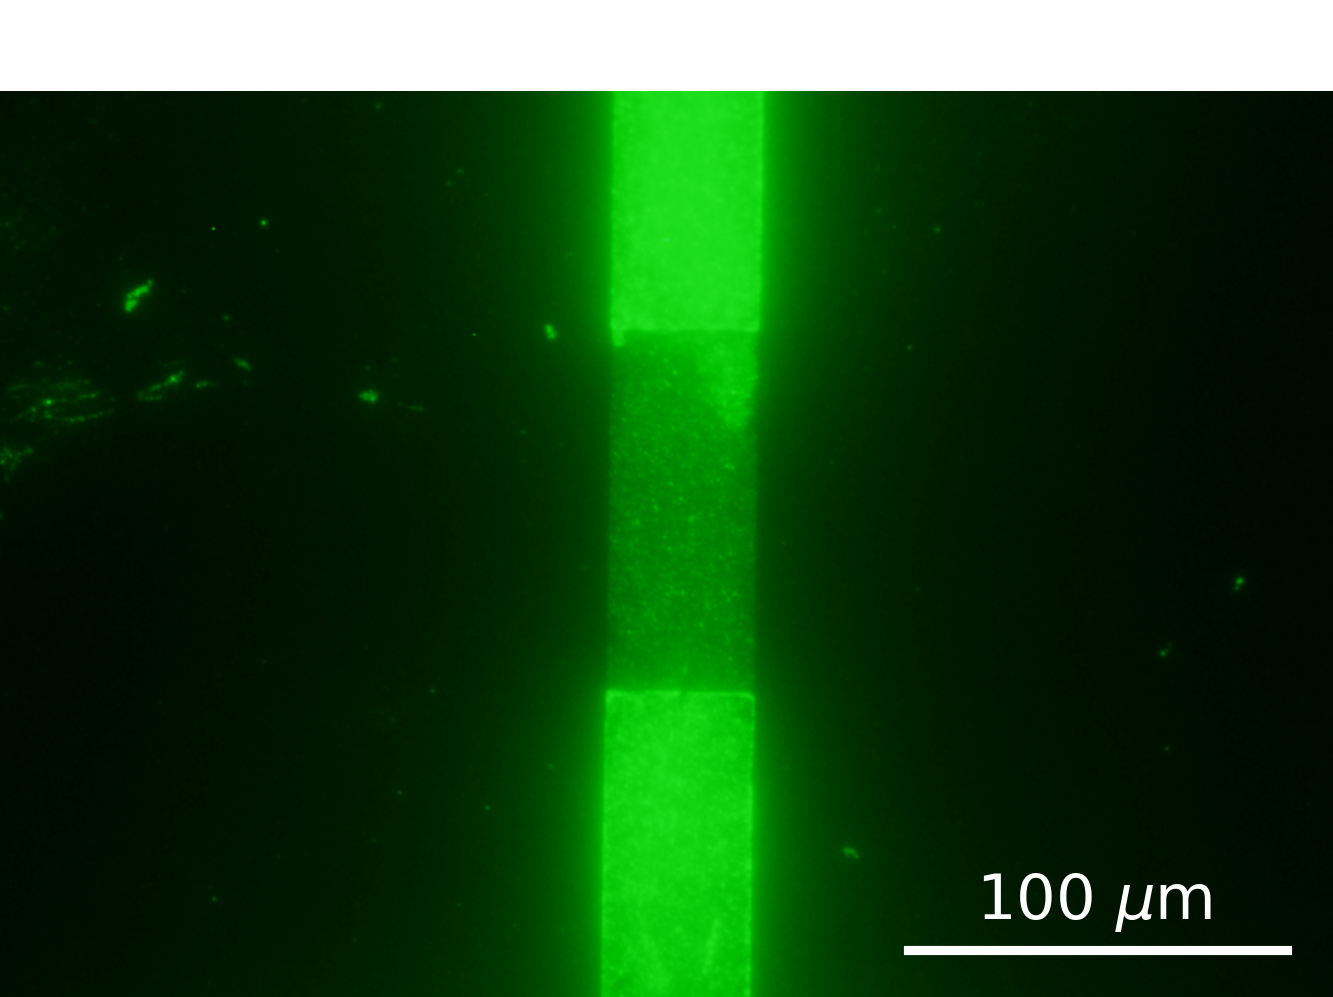
\includegraphics{figures/ch6/modified_GFPOR_PBASE_10sexposure_40X_mediumcontrast_ch2_231019.png}

}

}

\subcaption{\label{fig-PBASE-GFP-OR-ch2}}
\end{minipage}%
%
\begin{minipage}[t]{0.05\linewidth}

{\centering 

~

}

\end{minipage}%
%
\begin{minipage}[t]{0.47\linewidth}

{\centering 

\raisebox{-\height}{

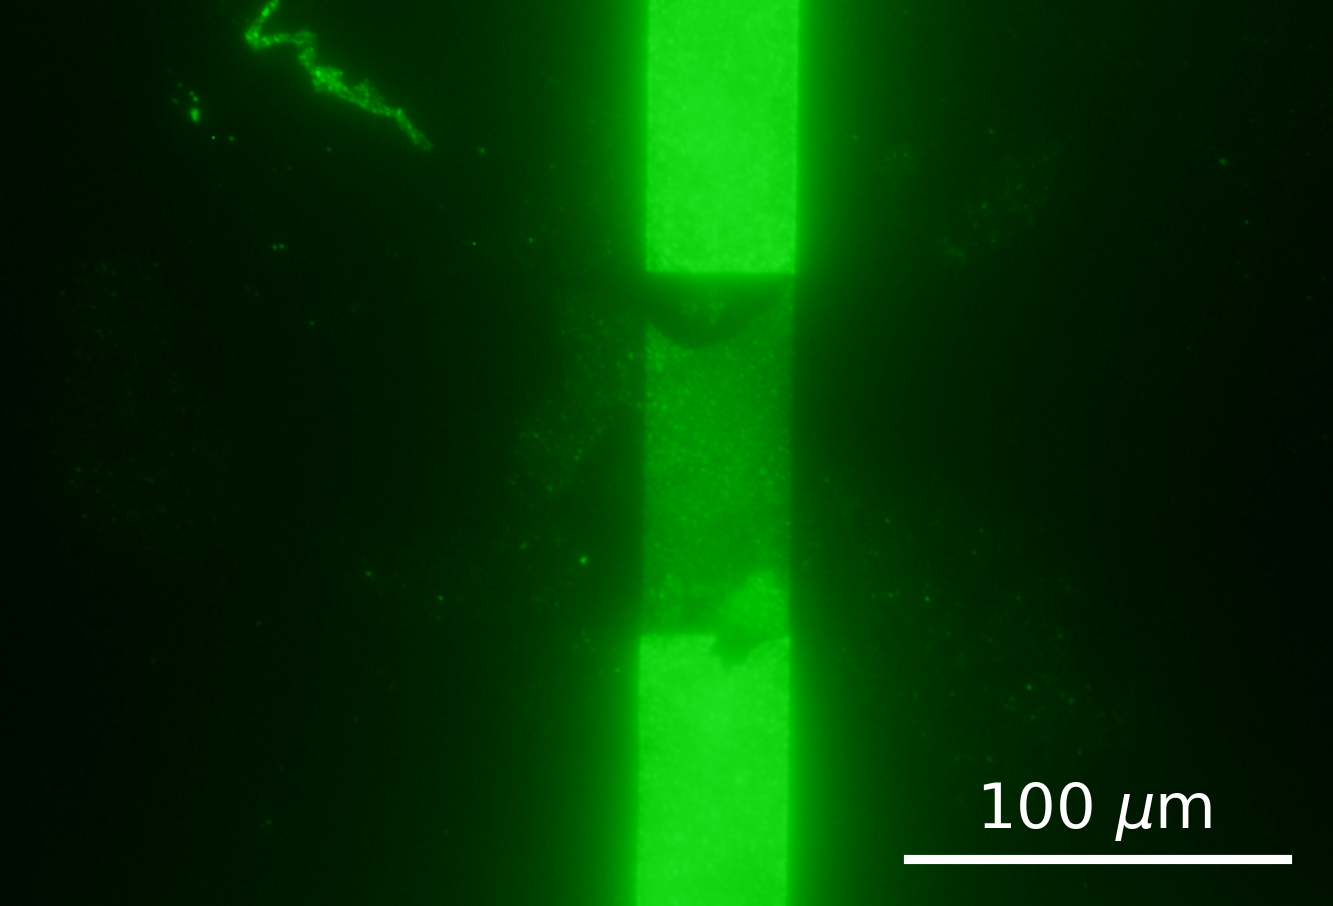
\includegraphics{figures/ch6/modified_GFPOR_PBASE_10sexposure_40X_mediumcontrast_ch3_231019.png}

}

}

\subcaption{\label{fig-PBASE-GFP-OR-ch3}}
\end{minipage}%
\newline
\begin{minipage}[t]{0.47\linewidth}

{\centering 

\raisebox{-\height}{

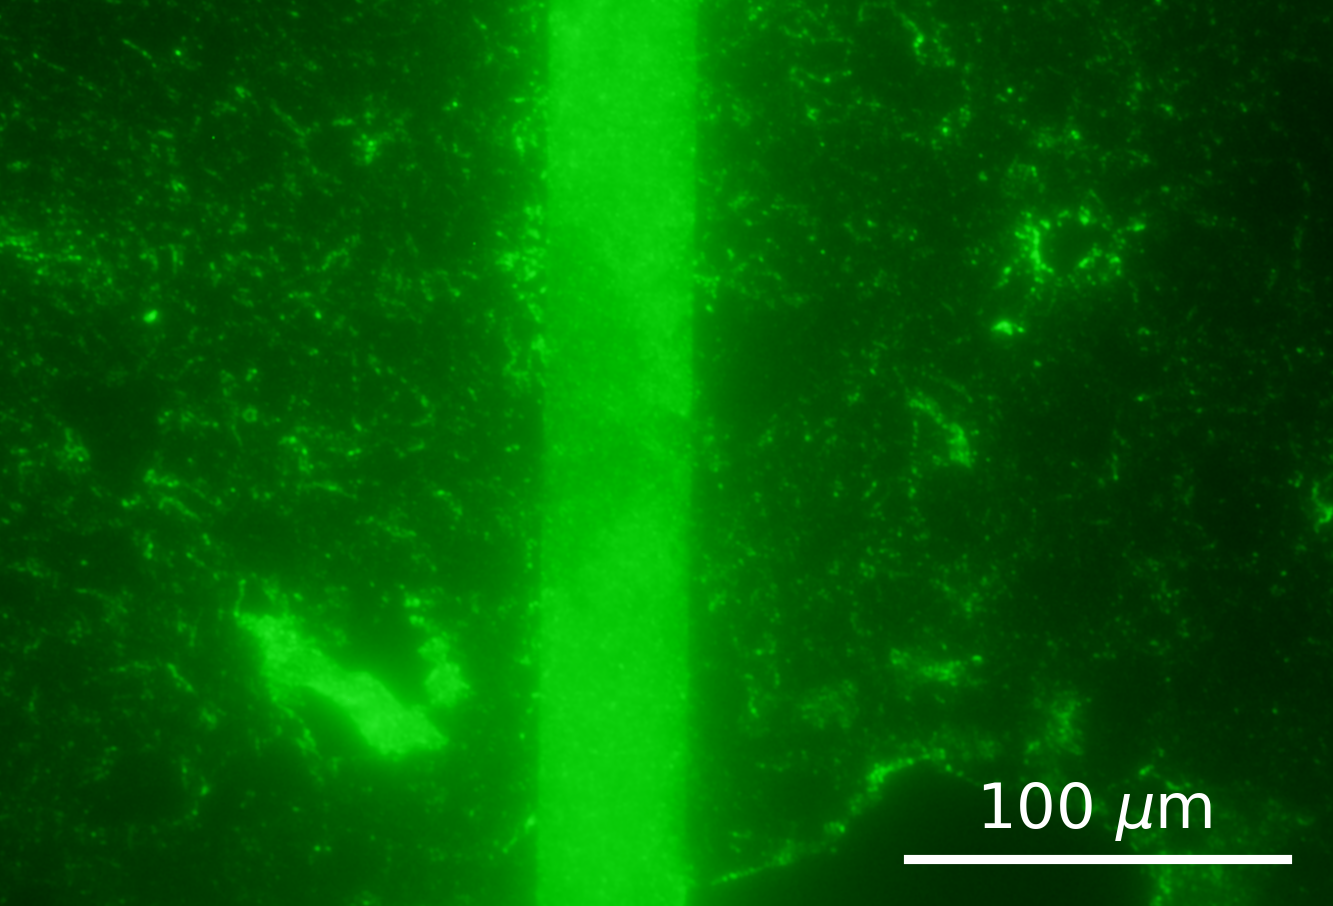
\includegraphics{figures/ch6/modified_GFPOR_PBASE_10sexposure_40X_mediumcontrast_ch6_231019.png}

}

}

\subcaption{\label{fig-PBASE-GFP-OR-ch6}}
\end{minipage}%
%
\begin{minipage}[t]{0.05\linewidth}

{\centering 

~

}

\end{minipage}%
%
\begin{minipage}[t]{0.47\linewidth}

{\centering 

\raisebox{-\height}{

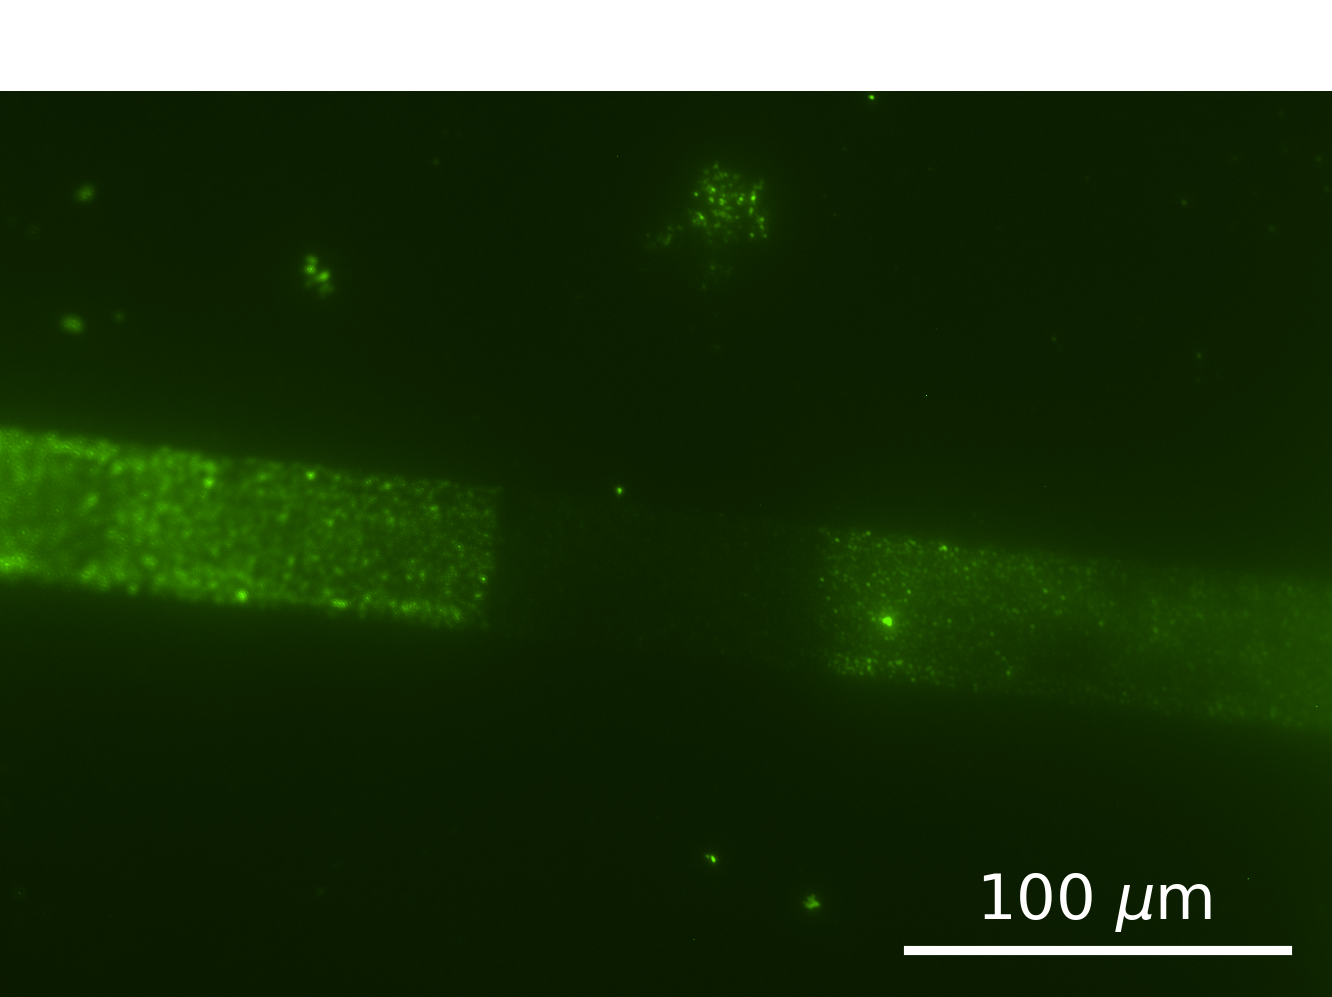
\includegraphics{figures/ch6/modified_GFPOR_10sexposure_40X_mediumcontrast_ch1_231027.png}

}

}

\subcaption{\label{fig-PBASE-GFP-OR-0.1mM}}
\end{minipage}%

\caption{\label{fig-PBASE-GFP-ORs}Fluorescence images of an
unencapsulated carbon nanotube network channel after functionalisation
with 1 mM PBASE in methanol, followed by 10 \(\mu\)L/mL GFP-OR43b
nanodiscs in 1XPBS.(a) and (b) show channel 1 of the device, (c) shows
channel 2, (d) shows channel 3 and (e) shows channel 6. The image in (f)
was taken of a separate device functionalised using 0.1 mM PBASE. All
images were taken using an GFP filter and a 10 s exposure time.}

\end{figure}

The functionalisation of unencapsulated carbon nanotube devices
(steam-deposited, fabricated after June 2023) with PBASE and GFP-OR
Nanodiscs was performed as follows:

\begin{enumerate}
\def\labelenumi{\arabic{enumi}.}
\item
  The device was exposed to UV light for 1 minute, placed in
  AZ\(^\circledR\) 326 developer for 3 minutes, then rinsed with
  acetone, isopropanol and nitrogen dried.
\item
  The device was vacuum annealed for 1 hour at 150\(^\circ\)C (Note:
  Steps 1 \& 2 were added to ensure any residual photoresist on the
  channel was removed or passivated before functionalisation, see
  Section~\ref{sec-photoresist-contamination}).
\item
  A solution of 1 mM PBASE (Setareh Biotech) in methanol prepared by
  fully dissolving 2 mg PBASE in 5 mL methanol by vortex mixing at 1000
  rpm in a dark room (Note: PBASE was stored at -18\(^\circ\)C for 18
  months prior to use, and was thawed under vacuum for 15 minutes in
  dark conditions before opening)
\item
  The device was then rinsed with methanol, fully submerged in \(\sim\)
  1 mL of PBASE in methanol solution and left covered with parafilm for
  1 hour, then rinsed with methanol for 15 s, rinsed with 1XPBS for 15 s
  and nitrogen dried to remove residual PBASE.
\item
  The device was left dry and in darkness while collecting the GFP-OR
  nanodiscs from the -80\(^\circ\)C freezer.
\item
  20 \(\mu\)L GFP-OR nanodiscs (batch number ND-GFP-OR43b-0002, prepared
  12 months earlier) was diluted in 2 mL 1XPBS (Note: The full 2 mL was
  used to flush out the nanodisc vial when preparing the nanodisc
  solution, with successive additions and subtractions of 50 \(\mu\)L
  1XPBS into and from the vial).
\item
  The device was submerged in the GFP-OR43b nanodisc solution and left
  covered with parafilm for 1 hour, then rinsed with 1XPBS for 15 s.
\item
  For fluorescence microscopy, the device was briefly rinsed with DI
  water and nitrogen dried to remove salt residue from the 1XPBS.
\end{enumerate}

Fluorescence images of the unencapsulated carbon nanotube devices
successfully functionalised with GFP-OR43b nanodiscs using PBASE are
shown in Figure~\ref{fig-PBASE-GFP-OR-ch3-zoom}-e.

As in Section~\ref{sec-PPF-fluorescence-characterisation}, dark regions
are the gold electrodes. There clearly appears to be an attachment
between the GFP-OR43b nanodiscs and the silicon dioxide surface. As this
device has been annealed, UV exposed and developed before
functionalisation, this non-specific attachment is unlikely to be
interaction with residual photoresist (see
Section~\ref{sec-photoresist-contamination}). Instead it appears that
the pyrene, nanodiscs or both are directly interacting with the silicon
dioxide surface. Fluorescence in the channel region in
Figure~\ref{fig-PBASE-GFP-OR-ch3-zoom}-e indicates GFP-OR43b nanodiscs
are present on or around the carbon nanotubes. The fluorescence
brightness was consistent across four out of eight channels on the 1 mM
PBASE functionalised device. The other four channels looked similar to
Figure~\ref{fig-PBASE-GFP-OR-ch6}, where nanodiscs appeared to be
present in excess on both the channel, SiO\(_2\), and even on the gold
electrodes. This is an indication that the concentration of GFP-OR43b
used should be lowered further for a more consistent functionalisation.

Figure~\ref{fig-PBASE-GFP-OR-0.1mM} shows that a lowered concentration
of PBASE leads to a channel region with no visible fluorescence (with a
10 s exposure time). This indicates that the PBASE solution used to
incubate the device must be sufficiently concentrated for odorant
receptors to interact with the channel region. As discussed in
Section~\ref{sec-pyrene-interactions}, this indicates that a specific
interaction is occurring between PBASE and the GFP-OR43b.

\hypertarget{sec-NTA-functionalisation}{%
\subsection{Functionalisation using
Pyrene-PEG-NTA}\label{sec-NTA-functionalisation}}

\begin{figure}

\begin{minipage}[t]{0.47\linewidth}

{\centering 

\raisebox{-\height}{

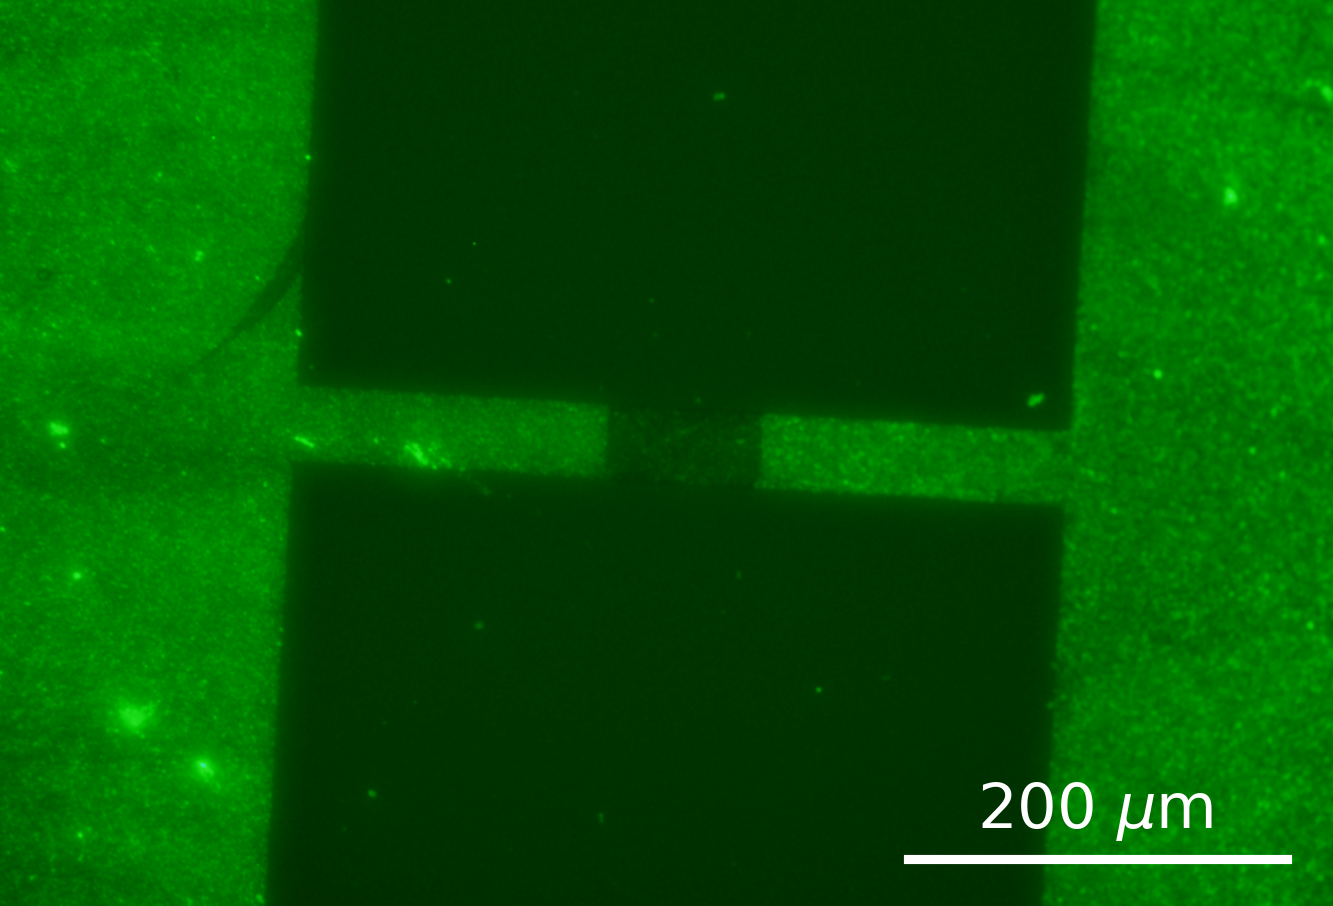
\includegraphics{figures/ch6/modified_GFPOR_Cu2+_10sexposure_20X_mediumcontrast_ch4_231027.png}

}

}

\subcaption{\label{fig-PPN-GFP-OR-1}}
\end{minipage}%
%
\begin{minipage}[t]{0.05\linewidth}

{\centering 

~

}

\end{minipage}%
%
\begin{minipage}[t]{0.47\linewidth}

{\centering 

\raisebox{-\height}{

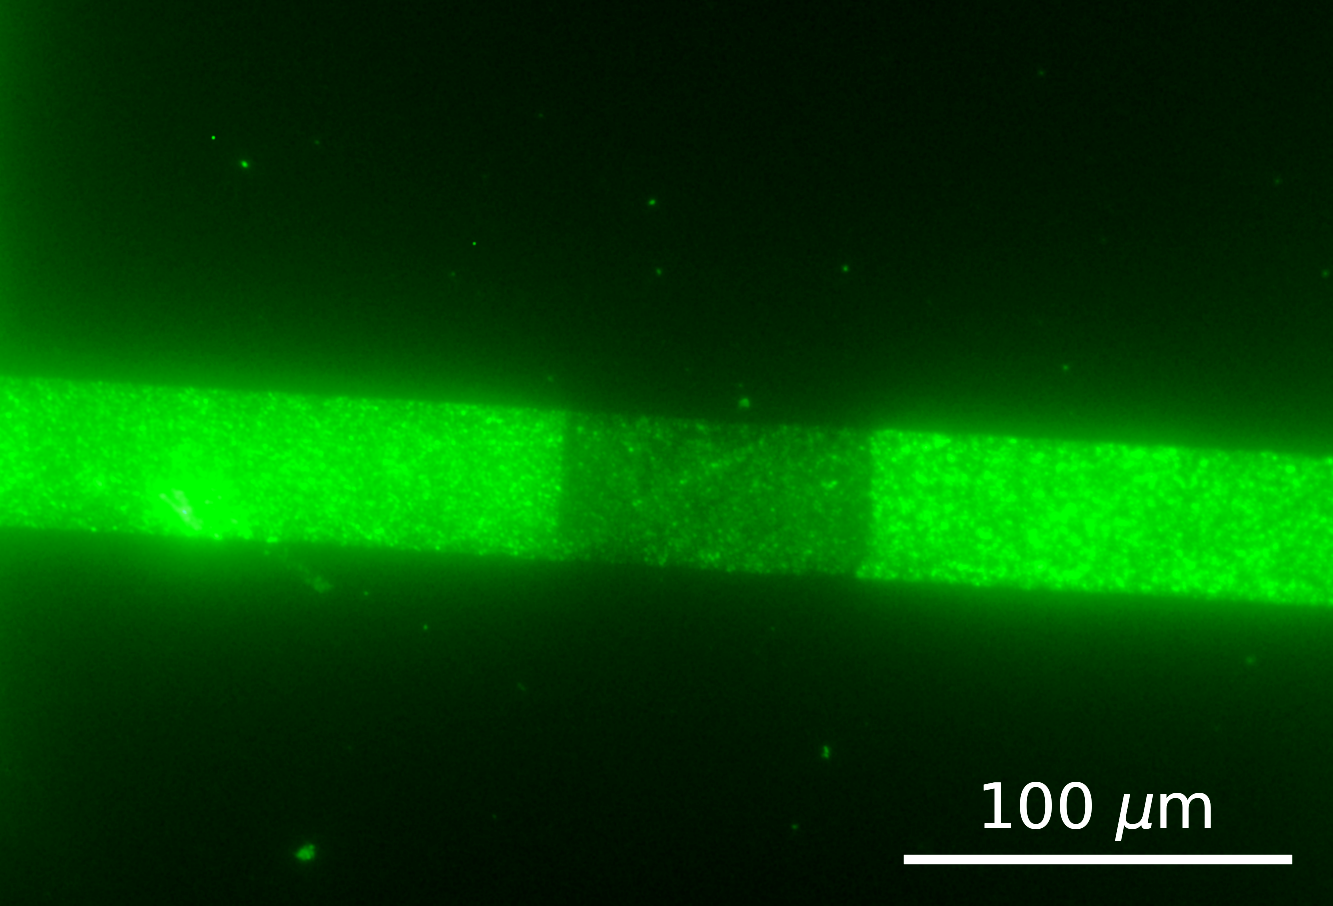
\includegraphics{figures/ch6/modified_GFPOR_Cu2+_10sexposure_40X_mediumcontrast_ch4_231027_40b.png}

}

}

\subcaption{\label{fig-PPN-GFP-OR-2}}
\end{minipage}%

\caption{\label{fig-OR-GFP-PPN}Image (a) and (b) show fluorescence
images of a carbon nanotube channel after functionalisation with 1
\(\mu\)L/mL GFP-OR43b nanodiscs in 1XPBS using pyrene-PEG-NTA. (b) has
been brightened by 40\% for visual clarity. Both images were taken using
a GFP filter and 10 s exposure time.}

\end{figure}

Pyrene-PEG-NTA was also used to attach the green fluorescent protein
tagged odorant receptors through attaching to their histidine tag via
the mechanisms outlined in Section~\ref{sec-NTA-biotin-PEG}. As
nanodiscs as well as odorant receptors have attached amine groups (see
\textbf{?@sec-artificial-membranes}), even nanodiscs which do not
contain the receptor required for sensing can attach to the carbon
nanotubes in the presence of PBASE linker. However, the nanodiscs used
here possessed no histidine tag. Therefore, successful GFP-OR Nanodisc
attachment via a histidine bonding process indicates odorant receptors,
rather than nanodisc membranes, have specifically attached to the carbon
nanotube network.

The following procedure was used to functionalise unencapsulated carbon
nanotube devices (steam-deposited, fabricated after June 2023) with
pyrene-PEG-NTA and GFP-OR nanodiscs:

\begin{enumerate}
\def\labelenumi{\arabic{enumi}.}
\item
  The device was exposed to UV light for 1 minute, placed in
  AZ\(^\circledR\) 326 developer for 3 minutes, then rinsed with
  acetone, isopropanol and nitrogen dried.
\item
  The device was vacuum annealed for 1 hour at 150\(^\circ\)C (Note:
  Steps 1 \& 2 were added to ensure any residual photoresist on the
  channel was removed or passivated before functionalisation, see
  Section~\ref{sec-photoresist-contamination}).
\item
  A solution of 100 \(\mu\)M Pyrene-PEG-NTA (Nanocs) in ethanol was
  prepared by fully dissolving 1 mg Pyrene-PEG-NTA in 5 mL ethanol by
  sonicating for 1 minute in a dark room (Note: Pyrene-PEG-NTA was
  stored at -18\(^\circ\)C for 6 months prior to use, and was thawed
  under vacuum for 15 minutes in dark conditions before opening; the
  solution was left at 4\(^\circ\)C for a week before use).
\item
  10 mL of 10 mM CuSO\(_4\) in 1XPBS was prepared by dissolving
  CuSO\(_4\) powder in 1XPBS by vortex mixing for 15 minutes.
\item
  After vortex mixing Pyrene-PEG-NTA in ethanol solution at 1000 rpm for
  10 minutes, the Pyrene-PEG-NTA solution was diluted to 1 \(\mu\)M in
  ethanol by placing 100 \(\mu\)L into 9.9 mL ethanol.
\item
  The device was then rinsed with acetone, IPA and nitrogen dried, fully
  submerged in 10 mL of 1 \(\mu\)M Pyrene-PEG-NTA in ethanol solution
  and left covered with parafilm for 15 minutes, then rinsed with
  ethanol for 15 s, rinsed with 1XPBS for 15 s and nitrogen dried to
  remove residual Pyrene-PEG-NTA.
\item
  The device was then placed in 10 mL of CuSO\(_4\) in 1XPBS and covered
  with parafilm for 1 hour to coordinate Cu\(^{2+}\) with NTA, then
  rinsed 15 with 1XPBS (Note: NiSO\(_4\) can be used as an alternative)
\item
  10 \(\mu\)L GFP-OR nanodiscs were diluted in 10 mL 1XPBS (batch number
  ND-GFP-OR43b-0002, prepared 12 months earlier and stored at
  -80\(^\circ\)C) .
\item
  The device was submerged in the GFP-OR43b nanodisc solution and left
  covered with parafilm for 30 minutes, then rinsed with 1XPBS for 15 s.
\item
  For fluorescence microscopy, the device was rinsed with DI water for 1
  minute and nitrogen dried to remove salt residue from the 1XPBS.
\end{enumerate}

Fluorescence images of the unencapsulated carbon nanotube devices
successfully functionalised with GFP-OR43b nanodiscs using
Pyrene-PEG-NTA are shown in Figure~\ref{fig-PPN-GFP-OR-1}-b. Similar
non-specific attachment to the silicon dioxide as in
Section~\ref{sec-PBASE-GFP-OR-attachment} is seen, but there is clear
attachment of green fluorescent protein-modified odorant receptors in
the channel. Device characteristics were measured with a multimeter to
check how the device characteristics changed during the
functionalisation process. The minimum measured channel resistance
increased from 560 k\(\Omega\) to 790 k\(\Omega\), indicating the
functionalisation process tends to decrease channel conductance.

\hypertarget{sec-conclusions}{%
\section{Conclusions}\label{sec-conclusions}}

It has been well-established in the literature that the \(\pi\)-stacking
reaction mechanism between pyrene-based linkers and graphene and carbon
nanotube network field-effect transistors can be used to create working
biosensors. The previous use of various linker molecules for biosensor
functionalisation was investigated. Despite the wide use of
1-pyrenebutanoic acid N-hydroxysuccinimide ester (PBASE) and
1-pyrenebutyric acid (PBA) for functionalisation of biosensors, the
literature shows a significant variation in the methods used for
attachment of linker molecules to a transistor channel. The most common
methods, using 6 mM PBASE dissolved in dimethylformamide or 1 mM PBASE
in methanol, stem directly from the first documented use of PBASE for
functionalisation of carbon nanotube biosensors. In the last 6 years,
more research has been done into optimising the PBASE methodology for
graphene devices, but there is still disagreement in the literature over
whether minimising or maximising PBASE coverage on a graphene device
channel is desirable for sensing. Due to disagreement in the literature
around suitable non-covalent methods for biosensor functionalisation,
several steps were taken to identify a rapid and simple method for
verifying successful functionalisation, and to locate any potential
barriers to a successful functionalisation.

I first compared the advantages and disadvantages of the various linker
molecules under investigation. The use of hydrogen NMR gave indications
that water was present in PBASE samples prepared in DMSO. Concerns
around the impact of the hydrolysis of PBASE on functionalisation mean
that the presence of water is strongly undesirable. An alternative
functionalisation approach less prone to hydrolysis is the reaction of
PBA with EDC in the presence of NHS. However, this process has its own
disadvantages, such as undesirable protein interactions and the
increased amount of steps and process variables involved. Pyrene-NTA is
also less prone to hydrolysis than PBASE but unlike PBASE or PBA/EDC
interacts with a specific protein tag, the histidine tag. PEGlyation of
the pyrene-NTA linker also means that the entire functionalisation
process can be performed in aqueous solution, avoiding the introduction
of non-organic solvents. This approach is desirable, since the
non-aqueous solvents traditionally used for functionalisation may have
negative impacts on device behaviour. For example, carbon nanotube
device channel transfer characteristics were found to undergo a
significant shift of \(\Delta V = -0.15 \pm 0.02\) when exposed to DMSO
or MeOH for 1 hour.

Next, I verified that the pyrene groups of the linker molecules of
interest were attaching successfully to either carbon nanotubes or
graphene. Raman spectroscopy showed that incubating a highly-bundled
carbon nanotube film in 5 mM PBASE or PBA in DMSO for 1 hour increased
I\(_D\)/I\(_G\) by a factor of \(\sim 3\) relative to the DMSO-only
case. Incubating a steam-deposited carbon nanotube device in a 1 mM
concentration of PBASE in methanol or DMSO for 1 hour was found to cause
a significant increase in device on-current relative to the solvent-only
case, and a similar increase in on-current was seen for 5 mM PBA in DMSO
relative to the DMSO-only case. When a PBA-functionalised device was
placed in aqueous solution with 20 mM EDC and 40 mM NHS for 30 minutes,
a further increase in on-current was seen. Fluorescence microscopy was
used to demonstrate the successful attachment of pyrene-PEG to graphene
using an attached FITC probe, where immersing a graphene film in 1 mM
pyrene-PEG in ethanol led to the channels becoming brightly fluorescent
relative to the background using a 1 s exposure time. Pyrene-PEG was
found to have little impact on the Dirac voltage of successfully
functionalised graphene devices.

Finally, I verified that the linkers were successfully attaching the
odorant receptors to the device channels with fluorescence microscopy.
Various obstacles to successful functionalisation were encountered and
addressed. Photoresist contamination was addressed with exposure and
development steps before functionalisation (no exposure for SU8
encapsulated devices). Hydrophobicity of graphene films was addressed by
plasma treatment before functionalisation in aqueous solution. A
surfactant rinse was used to distinguish between weak substrate-linker
interaction and \(\pi\)-stacking between linker and the channel.
Finally, coffee-ring distribution of linker was addressed by always
submerging the device in linker when functionalising. Once these issues
were addressed, two processes were identified which could be
demonstrated to be successful using fluorescence microscopy. The first
used an initial submersion in 1 mM PBASE in methanol for 1 hour, then
submersion in 10 \(\mu\)L mL\(^{-1}\) OR43b nanodiscs in 1XPBS for 1
hour. The second used a submersion in 1 \(\mu\)L pyrene-PEG-NTA in
ethanol for 15 minutes, then submersion in 10 mM CuSO\(_4\) in 1XPBS for
1 hour, then submersion in 1 \(\mu\)L mL\(^{-1}\) OR43b nanodiscs in
1XPBS for 30 minutes.

\cleardoublepage
\phantomsection
\addcontentsline{toc}{part}{Appendices}
\appendix

\hypertarget{sec-python}{%
\chapter{Python Code for Data Analysis}\label{sec-python}}

\hypertarget{code-repository}{%
\section{Code Repository}\label{code-repository}}

The code used for general analysis of field-effect transistor devices in
this thesis was written with Python 3.8.8. Contributors to the code used
include Erica Cassie, Erica Happe, Marissa Dierkes and Leo Browning. The
code is located on GitHub and the research group OneDrive, and is
available on request.

\hypertarget{sec-histogram-analysis}{%
\section{Atomic Force Microscope Histogram
Analysis}\label{sec-histogram-analysis}}

The purpose of this code is to analyse atomic force microscope (AFM)
images of carbon nanotube networks in .xyz format taken using an atomic
force microscope and processed in Gwyddion (see
\textbf{?@sec-afm-characterisation}). It was originally designed by
Erica Happe in Matlab, and adapted by Marissa Dierkes and myself for use
in Python. The code imports the .xyz data and sorts it into bins 0.15 nm
in size for processing. To perform skew-normal distribution fits, both
\emph{scipy.optimize.curve\_fit} and \emph{scipy.stats.skewnorm} modules
are used in this code.

\hypertarget{sec-raman-analysis}{%
\section{Raman Spectroscopy Analysis}\label{sec-raman-analysis}}

The purpose of this code is to analyse a series of Raman spectra taken
at different points on a single film (see
\textbf{?@sec-raman-characterisation}). Data is imported in a series of
tab-delimited text files, with the low wavenumber spectrum (100
cm\(^{-1} - 650\) cm\(^{-1}\)) and high wavenumber spectrum (1300
cm\(^{-1} - 1650\) cm\(^{-1}\)) imported in separate datafiles for each
scan location.

\hypertarget{sec-field-effect-transistor-analysis}{%
\section{Field-Effect Transistor
Analysis}\label{sec-field-effect-transistor-analysis}}

The purpose of this code is to analyse electrical measurements taken of
field-effect transistor (FET) devices. Electrical measurements were
either taken from the Keysight 4156C Semiconductor Parameter Analyser,
National Instruments NI-PXIe or Keysight B1500A Semiconductor Device
Analyser as discussed in \textbf{?@sec-electrical-characterisation}; the
code is able to analyse data taken from all three measurement setups.
The main Python file in the code base consists of three related but
independent modules: the first analyses and plots sensing data from the
FET devices, the second analyses and plots transfer characteristics from
channels across a device, and the third compares individual channel
characteristics before and after a modification or after each of several
modifications. The code base also features a separate config file and
style sheet which govern the behaviour of the main code. The code base
was designed collaboratively by myself and Erica Cassie over GitHub
using the Sourcetree Git GUI.

The first of the three modules is for processing sensing datasets. This
module imports sensing measurements in .csv format and analyses them,
then outputs a plot of the raw data, alongside multiple plots which have
been modified in various ways. It can also fit exponential and linear
trendlines to regions of the sensing data, as well as find the signal
change per analyte addition, and returns spreadsheets containing the
results of these analyses. These spreadsheets include the standard
deviation for all included parameters. Modified plots include normalised
plots (type of normalisation can be set in config file), plots with
fitted curves, plots with the linear baseline drift removed, plots of
signal with analyte addition, ``despiked'' plots and ``filtered'' plots.
It is possible to add annotations to any of these plots using the config
file, and it is possible to produce a plot with a combination of these
modifications.

The scipy.optimize.curve\_fit module is used to fit linear and
exponential curves to regions of interest of the sensing data. Initial
parameters for the scipy.optimize.curve\_fit module are chosen by
approximating fitting parameters in a similar manner to the approach in
Section~\ref{sec-histogram-analysis}. For a linear fit \(mt + b\), the
parameters are simply set as \(m=1\) and \(b=0\). For an exponential fit
\(a\exp{(-t/\tau)} + c\), \(c\) is set as the final current measurement
of the region of interest and \(a\) is set as the initial current
measurement minus \(c\). Then, \(\tau\) is set as the time where current
has dropped to \(e^{-1}a + c\).

``Despiked'' plots have had spurious datapoints removed through the use
of an interquartile range rolling filter. The window size of the rolling
filter used was 40 datapoints, and datapoints in each window with a
z-score above \(\pm 3\) were removed from the plotted/processed data.
``Filtered'' plots had noise reduced using a moving median filter. The
moving median filter is more effective at removing noise than a simple
moving average, and has advantages over other filters (such as the
Savitzky-Golay filter) when removing noise from data with sharp edges,
as is the case for sensing data. Median filtering can also be used for
baseline drift compensation, though this approach was not used in this
thesis \autocite{Stone2011}. The moving median filter used had a window
of 40 datapoints.

Plots of signal with analyte addition were constructed from current data
after first removing baseline drift and applying a moving median filter.
A simple difference calculation between the mean of the filtered current
before an addition and the mean of the filtered current after the
addition was performed at each addition. These differences were then
normalised relative to the initial current. The signal with analyte
addition give reasonably consistent results regardless of whether
baseline drift was removed from the data, as shown in
Figure~\ref{fig-spaa-plot-comparison}. We can therefore be confident
that robust signal with analyte addition plots are robust even in the
presence of significant drift.

\begin{figure}

\begin{minipage}[t]{0.50\linewidth}

{\centering 

\raisebox{-\height}{

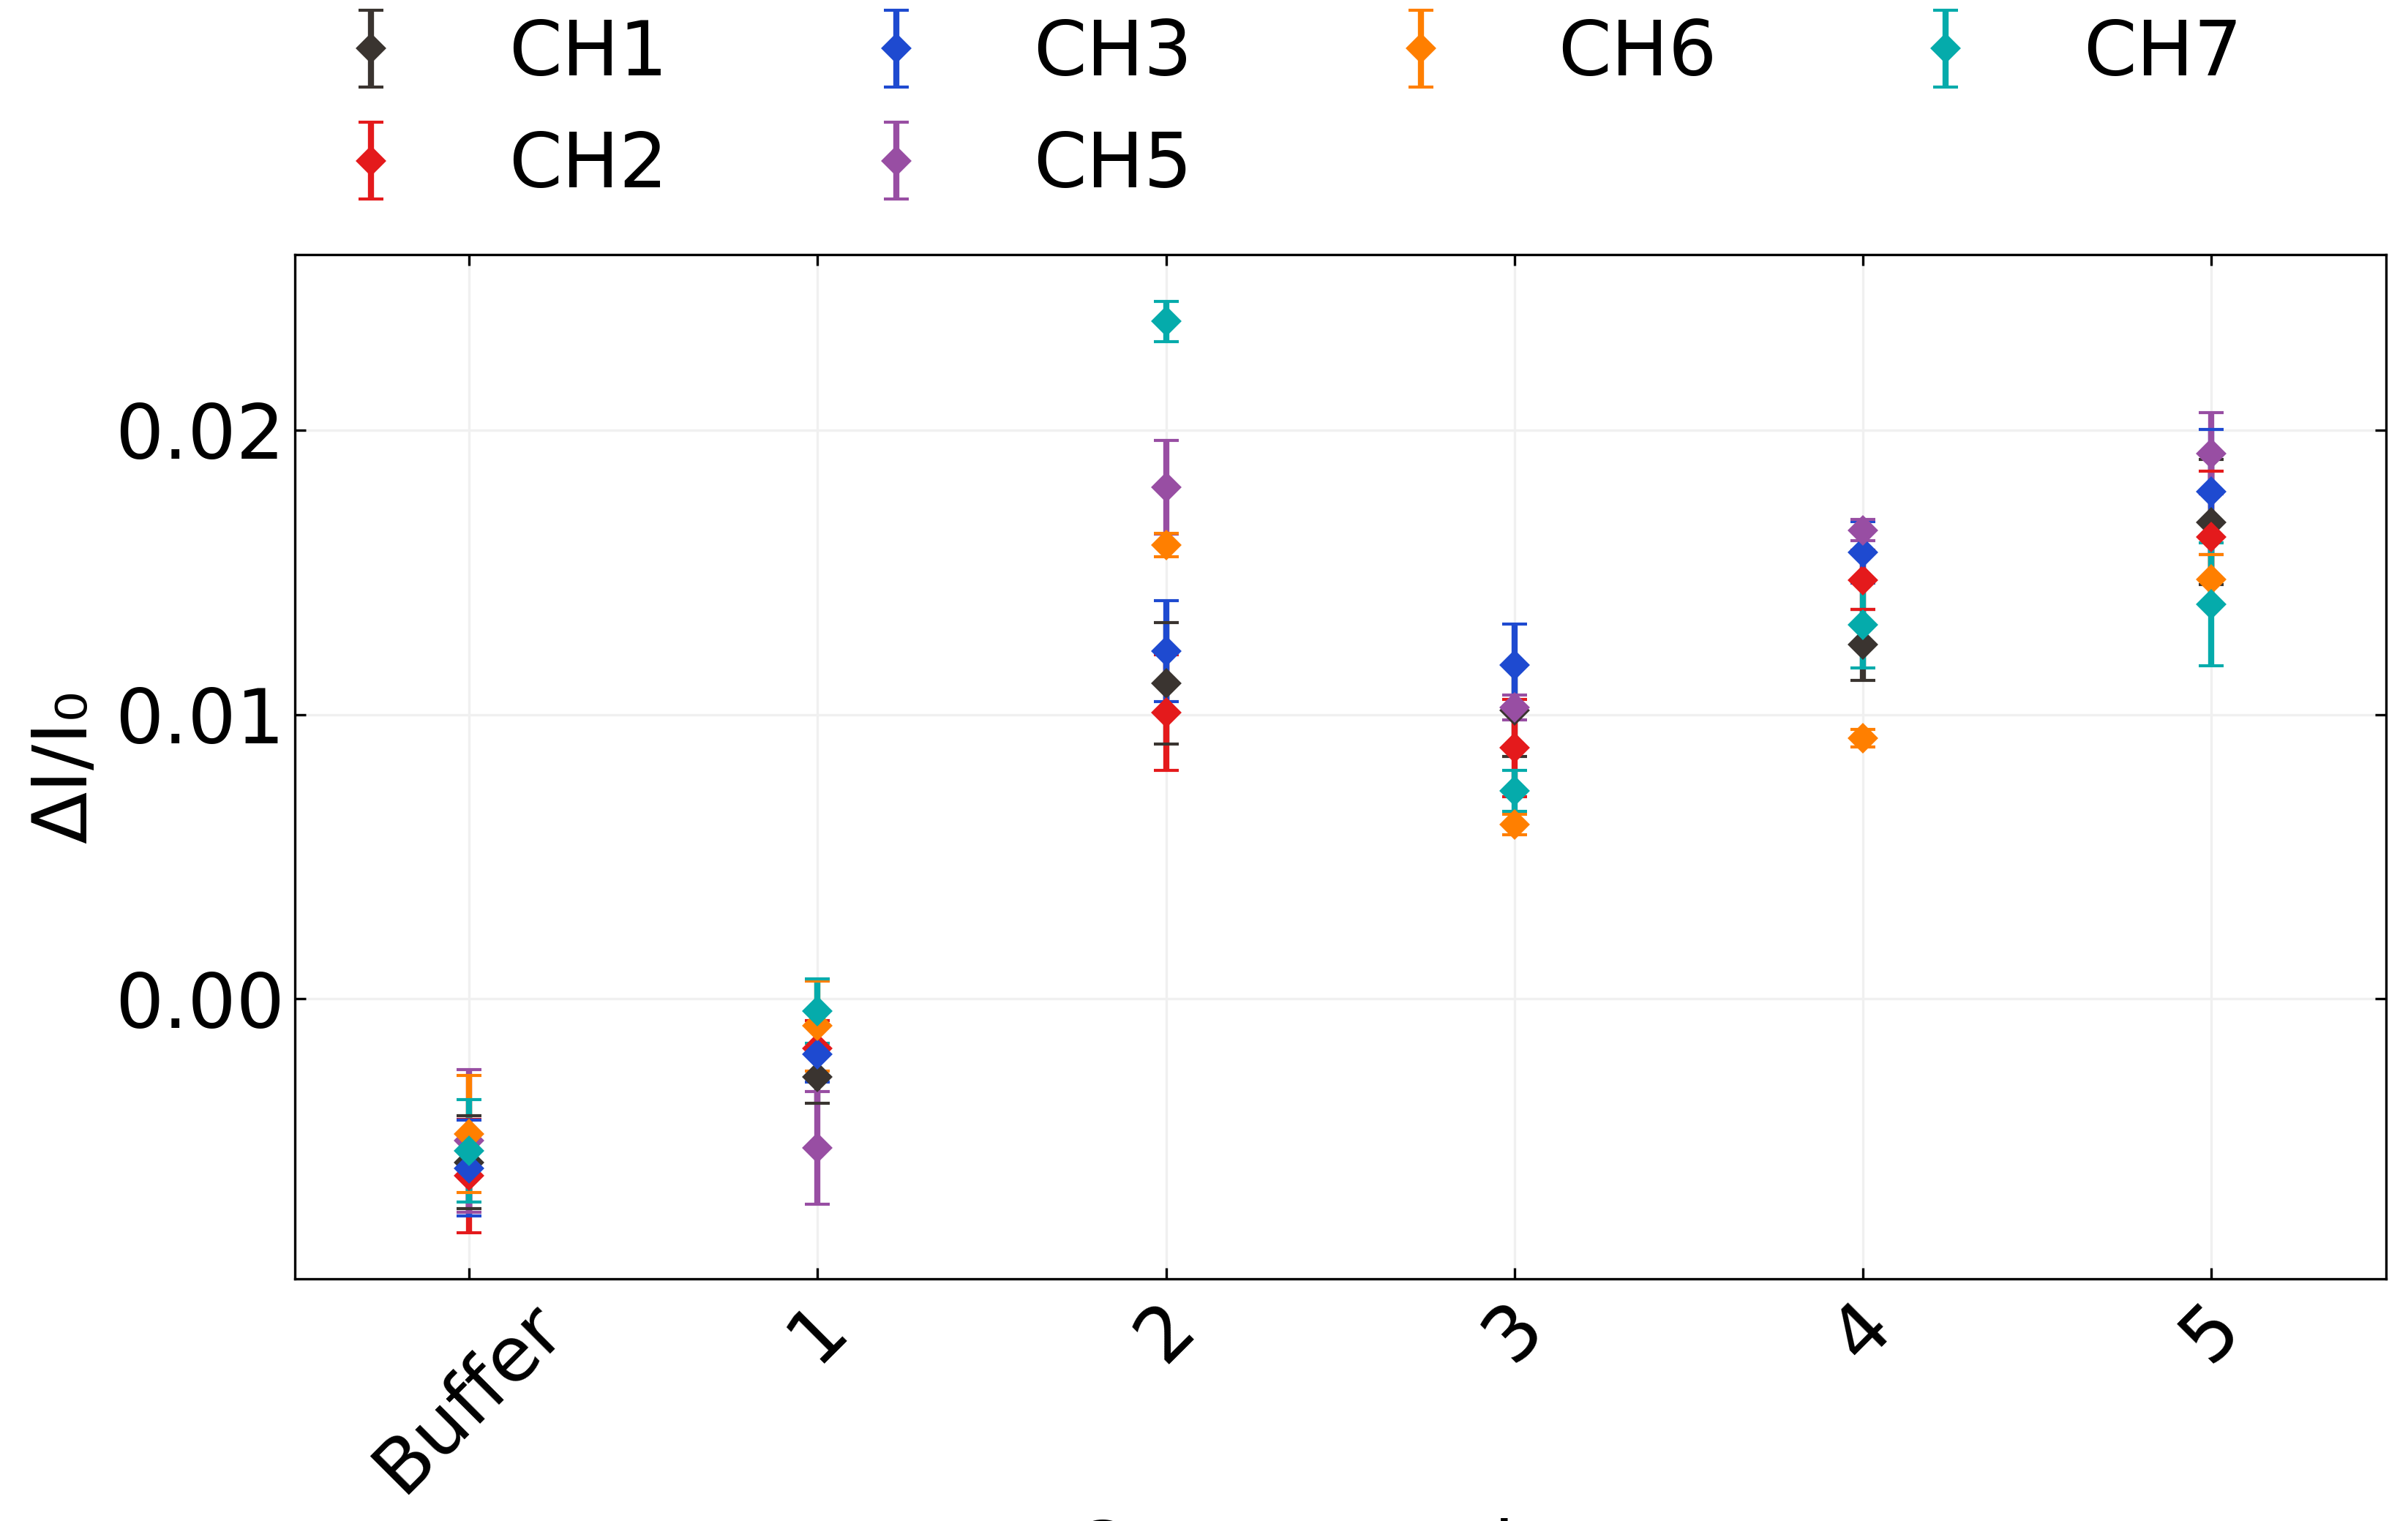
\includegraphics{figures/app1/NTQ31C1_mean_simple_difference_before_and_after_step_filtered_concentrations.png}

}

}

\subcaption{\label{fig-spaa-no-detrend}}
\end{minipage}%
%
\begin{minipage}[t]{0.50\linewidth}

{\centering 

\raisebox{-\height}{

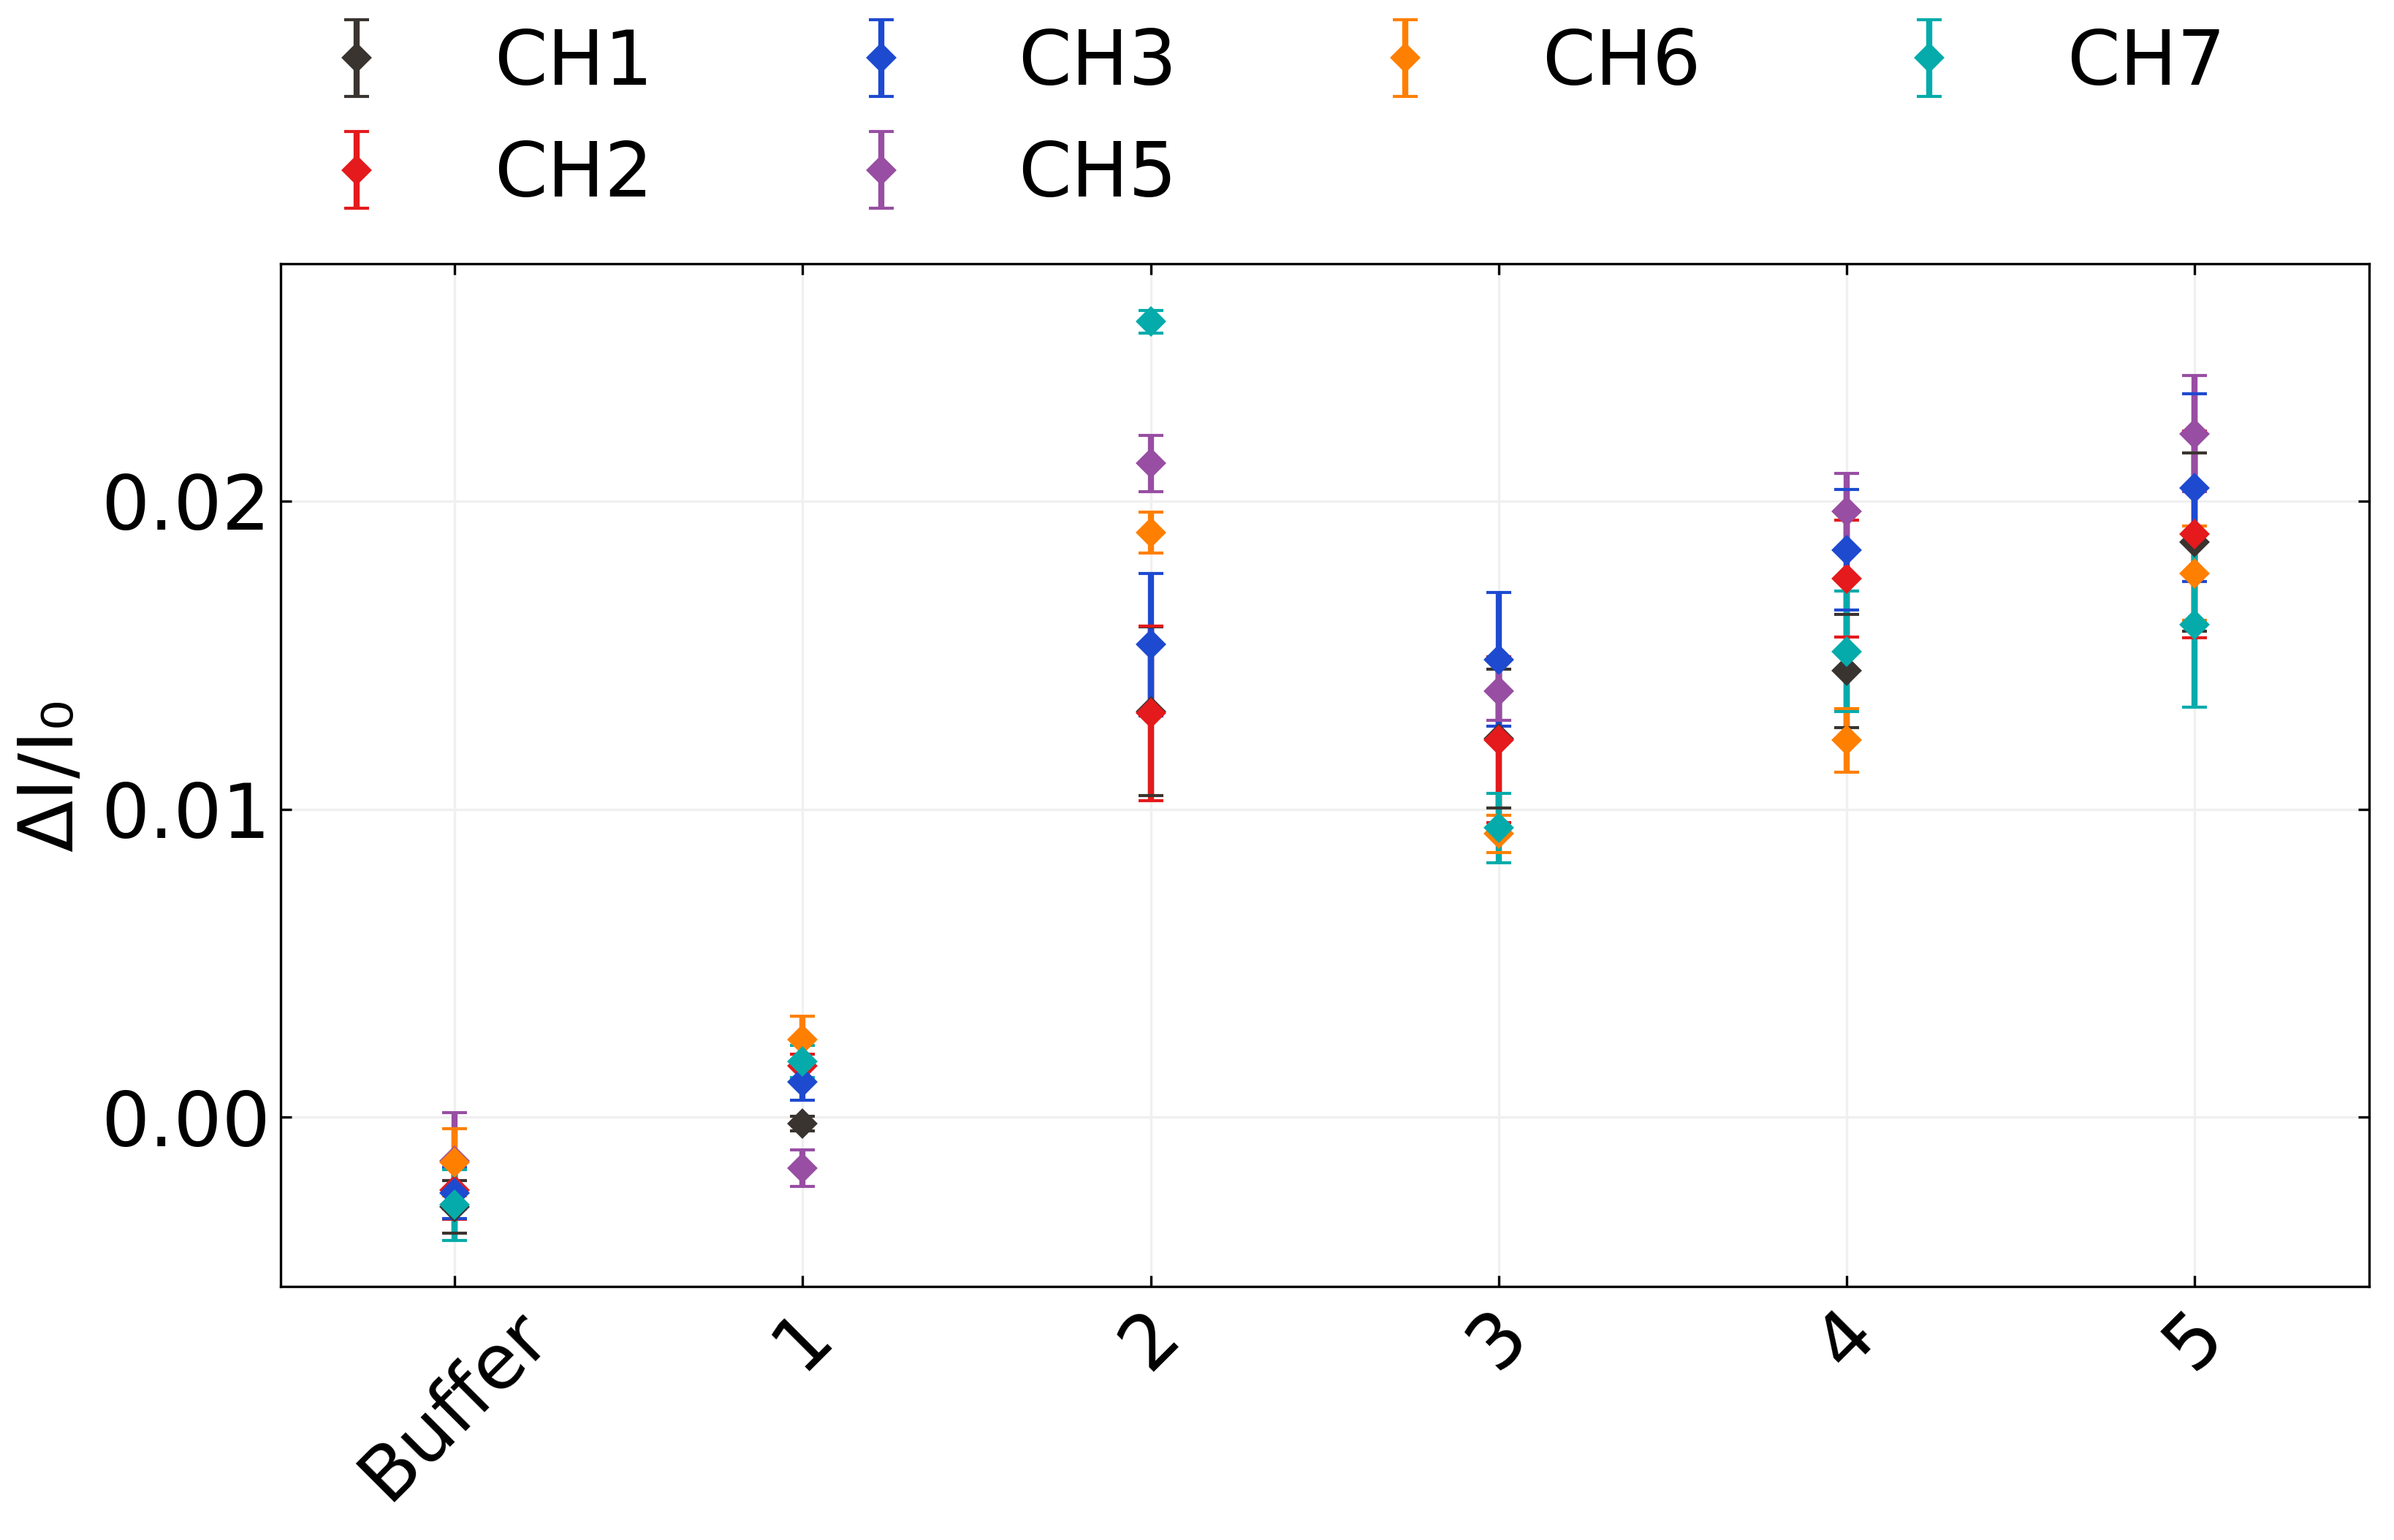
\includegraphics{figures/app1/NTQ31C1_mean_simple_difference_before_and_after_step_filtered_concentrations_detrend.png}

}

}

\subcaption{\label{fig-spaa-detrend}}
\end{minipage}%

\caption{\label{fig-spaa-plot-comparison}A comparison of signal with
analyte addition plots taken from the same salt concentration sensing
dataset (the same dataset as used in \textbf{?@fig-salt-conc-sensing}).
In (a), a simple difference calculation performed on filtered data was
used, while in (b) the same calculation was performed on filtered data
with the baseline drift removed, the method used in the body of the
thesis.}

\end{figure}

The second module imports transfer measurements in .csv format and
creates combined and individual plots of the eight channels on a single
device. In combined plots, channels which are non-working, due to being
shorted or non-conducting, are removed via setting a maximum and minimum
possible on-current in the config file. Various parameters from the
transfer characteristics are saved as a spreadsheet along with standard
error. These parameters include on current, off current, subthreshold
slope and threshold voltage for the carbon nanotube devices, and on
current, off current and major Dirac point voltage for graphene devices.
The device type being analysed can be set in the config file.

The third module imports several transfer measurements in .csv format
and allows for comparison of the same channel before and after some
modification. It also calculates the shift in either threshold voltage
or major Dirac voltage of the device.


\backmatter
\printbibliography


\end{document}
